%%%%%%%%%%%%%%%%%%%%%%%%%%%%%%%%%%%%%%%%%
% Classicthesis Typographic Thesis
% LaTeX Template
% Version 1.3 (15/2/14)
%
% This template has been downloaded from:
% http://www.LaTeXTemplates.com
%
% Original author:
% André Miede (http://www.miede.de)
%
% License:
% CC BY-NC-SA 3.0 (http://creativecommons.org/licenses/by-nc-sa/3.0/)
%
% General Tips:
% 1) Make sure to edit the classicthesis-config.file
% 2) New enumeration (A., B., C., etc in small caps): \begin{aenumerate} \end{aenumerate}
% 3) For margin notes: \marginpar or \graffito{}
% 4) Do not use bold fonts in this style, it is designed around them
% 5) Use tables as in the examples
% 6) See classicthesis-preamble.sty for useful commands
%
%%%%%%%%%%%%%%%%%%%%%%%%%%%%%%%%%%%%%%%%%

%----------------------------------------------------------------------------------------
%	PACKAGES AND OTHER DOCUMENT CONFIGURATIONS
%----------------------------------------------------------------------------------------

\documentclass[
		twoside,openright,titlepage,numbers=noenddot,headinclude,%1headlines,
                footinclude=true,cleardoublepage=empty,
                BCOR=5mm,paper=a4,fontsize=11pt, % Binding correction, paper type and font size
                ngerman,english, % Languages
                ]{scrreprt}

% Includes the file which contains all the document configurations and packages - make sure to edit this file
%%%%%%%%%%%%%%%%%%%%%%%%%%%%%%%%%%%%%%%%%
% Thesis Configuration File
%
% The main lines to change in this file are in the DOCUMENT VARIABLES
% section, the rest of the file is for advanced configuration.
%
%%%%%%%%%%%%%%%%%%%%%%%%%%%%%%%%%%%%%%%%%

%----------------------------------------------------------------------------------------
%	DOCUMENT VARIABLES
%	Fill in the lines below to enter your information into the thesis template
%	Each of the commands can be cited anywhere in the thesis
%----------------------------------------------------------------------------------------

\PassOptionsToPackage{utf8x}{inputenc}
\usepackage{inputenc}

% Remove drafting to get rid of the '[ Date - classicthesis version 4.0 ]' text at the bottom of every page
\PassOptionsToPackage{eulerchapternumbers,listings,drafting,pdfspacing, subfig,beramono,parts,dottedtoc}{classicthesis}
% Available options: drafting parts nochapters linedheaders eulerchapternumbers beramono eulermath pdfspacing minionprospacing tocaligned dottedtoc manychapters listings floatperchapter subfig
% Adding 'dottedtoc' will make page numbers in the table of contents flushed right with dots leading to them

\newcommand{\myTitle}{Active Magnetic Field Stabilisation and Axion Dark Matter Search\xspace}
\newcommand{\mySubtitle}{My Subtitle\xspace}
\newcommand{\myDegree}{Doktor-Ingenieur (Dr.-Ing.)\xspace}
\newcommand{\myName}{Michał Rawlik\xspace}
\newcommand{\myProf}{Klaus Kirch\xspace}
\newcommand{\myOtherProf}{Put name here\xspace}
\newcommand{\mySupervisor}{Put name here\xspace}
\newcommand{\myFaculty}{Put data here\xspace}
\newcommand{\myDepartment}{Put data here\xspace}
\newcommand{\myUni}{Put data here\xspace}
\newcommand{\myLocation}{Zürich\xspace}
\newcommand{\myTime}{April~2018\xspace}
\newcommand{\myVersion}{early draft\xspace}

%----------------------------------------------------------------------------------------
%	USEFUL COMMANDS
%----------------------------------------------------------------------------------------

\newcommand{\ie}{i.\,e.}
\newcommand{\Ie}{I.\,e.}
\newcommand{\eg}{e.\,g.}
\newcommand{\Eg}{E.\,g.}

\newcounter{dummy} % Necessary for correct hyperlinks (to index, bib, etc.)
\providecommand{\mLyX}{L\kern-.1667em\lower.25em\hbox{Y}\kern-.125emX\@}

% Define a note environment for in-line comments.
\newcommand{\note}[1]{{\color{blue}[#1]}}
\newcommand{\mnote}[1]{{\marginpar{\color{blue}#1}}}
% Uncomment the line below to hide the notes in the produced file.
%\renewcommand{\note}[1]{}
%\renewcommand{\mnote}[1]{}

%----------------------------------------------------------------------------------------
%	PACKAGES
%----------------------------------------------------------------------------------------

\usepackage{lipsum} % Used for inserting dummy 'Lorem ipsum' text into the template

%------------------------------------------------

\PassOptionsToPackage{english}{babel}  % Change this to your language(s)
% Spanish languages need extra options in order to work with this template
%\PassOptionsToPackage{spanish,es-lcroman}{babel}
\usepackage{babel}

%------------------------------------------------

\PassOptionsToPackage{square,numbers}{natbib}
 \usepackage{natbib}

 %------------------------------------------------

\PassOptionsToPackage{fleqn}{amsmath} % Math environments and more by the AMS
\usepackage{amsmath}
\usepackage{amssymb}
\usepackage{upgreek}
\newcommand{\vtr}[1]{\boldsymbol{#1}}  %bold-math for vectors
\newcommand{\appropto}{\mathrel{\vcenter{
  \offinterlineskip\halign{\hfil$##$\cr
    \propto\cr\noalign{\kern2pt}\sim\cr\noalign{\kern-2pt}}}}}

 %------------------------------------------------

\PassOptionsToPackage{T1}{fontenc} % T2A for cyrillics
\usepackage{fontenc}

%------------------------------------------------

\usepackage{xspace} % To get the spacing after macros right

%------------------------------------------------

\usepackage{mparhack} % To get marginpar right

%------------------------------------------------

\usepackage{fixltx2e} % Fixes some LaTeX stuff

%------------------------------------------------

\PassOptionsToPackage{smaller}{acronym} % Include printonlyused in the first bracket to only show acronyms used in the text
\usepackage{acronym} % nice macros for handling all acronyms in the thesis

%------------------------------------------------

% \renewcommand*{\acsfont}[1]{\textssc{#1}} % For MinionPro
% \renewcommand{\bflabel}[1]{{#1}\hfill} % Fix the list of acronyms

%------------------------------------------------

\PassOptionsToPackage{pdftex}{graphicx}
\usepackage{graphicx}

%------------------------------------------------

\usepackage{units}
\usepackage{siunitx}
% \sisetup{detect-all} % use the current font for typesetting
\sisetup{detect-weight, detect-family, detect-shape} % use the current font for typesetting
% detect-all additionally sets detect-mode to true. I want this to be false - always use the math mode font for numbers with units. In the text the figures are normally non-lining, but I don't want that with units.
\usepackage{textcomp}
\usepackage{gensymb}
% ref. https://tex.stackexchange.com/questions/219310/too-many-math-alphabets-used-in-version-normal-when-using-4-packages-only
\newcommand\bmmax{2}
\usepackage{bm}

%------------------------------------------------


%----------------------------------------------------------------------------------------
%	FLOATS: TABLES, FIGURES AND CAPTIONS SETUP
%----------------------------------------------------------------------------------------

\usepackage{tabularx} % Better tables
\setlength{\extrarowheight}{3pt} % Increase table row height
\newcommand{\tableheadline}[1]{\multicolumn{1}{c}{\spacedlowsmallcaps{#1}}}
\newcommand{\myfloatalign}{\centering} % To be used with each float for alignment
\usepackage{caption}
\captionsetup{format=hang,font=small}
\usepackage{sidecap}
% for captions on the side don't let the caption hang
\captionsetup[SCfigure]{format=plain}
\usepackage{subfig}

%----------------------------------------------------------------------------------------
%	CODE LISTINGS SETUP
%----------------------------------------------------------------------------------------

\usepackage{listings}
%\lstset{emph={trueIndex,root},emphstyle=\color{BlueViolet}}%\underbar} % for special keywords
\lstset{language=[LaTeX]Tex, % Specify the language for listings here
keywordstyle=\color{RoyalBlue}, % Add \bfseries for bold
basicstyle=\small\ttfamily, % Makes listings a smaller font size and a different font
%identifierstyle=\color{NavyBlue}, % Color of text inside brackets
commentstyle=\color{Green}\ttfamily, % Color of comments
stringstyle=\rmfamily, % Font type to use for strings
numbers=left, % Change left to none to remove line numbers
numberstyle=\scriptsize, % Font size of the line numbers
stepnumber=5, % Increment of line numbers
numbersep=8pt, % Distance of line numbers from code listing
showstringspaces=false, % Sets whether spaces in strings should appear underlined
breaklines=true, % Force the code to stay in the confines of the listing box
%frameround=ftff, % Uncomment for rounded frame
frame=single, % Frame border - none/leftline/topline/bottomline/lines/single/shadowbox/L
belowcaptionskip=.75\baselineskip % Space after the "Listing #: Desciption" text and the listing box
}

%----------------------------------------------------------------------------------------
%	HYPERREFERENCES
%----------------------------------------------------------------------------------------

\PassOptionsToPackage{pdftex,hyperfootnotes=false,pdfpagelabels}{hyperref}
\usepackage{hyperref}  % backref linktocpage pagebackref
\pdfcompresslevel=9
\pdfadjustspacing=1

\hypersetup{
% Uncomment the line below to remove all links (to references, figures, tables, etc)
%draft,
colorlinks=true, linktocpage=true, pdfstartpage=3, pdfstartview=FitV,
% Uncomment the line below if you want to have black links (e.g. for printing black and white)
%colorlinks=false, linktocpage=false, pdfborder={0 0 0}, pdfstartpage=3, pdfstartview=FitV,
breaklinks=true, pdfpagemode=UseNone, pageanchor=true, pdfpagemode=UseOutlines,
plainpages=false, bookmarksnumbered, bookmarksopen=true, bookmarksopenlevel=1,
hypertexnames=true, pdfhighlight=/O, urlcolor=webbrown, linkcolor=RoyalBlue, citecolor=webgreen,
%------------------------------------------------
% PDF file meta-information
pdftitle={\myTitle},
pdfauthor={\textcopyright\ \myName, \myUni, \myFaculty},
pdfsubject={},
pdfkeywords={},
pdfcreator={pdfLaTeX},
pdfproducer={LaTeX with hyperref and classicthesis}
%------------------------------------------------
}

%----------------------------------------------------------------------------------------
%	BACKREFERENCES
%----------------------------------------------------------------------------------------

\usepackage{ifthen} % Allows the user of the \ifthenelse command
\newboolean{enable-backrefs} % Variable to enable backrefs in the bibliography
\setboolean{enable-backrefs}{false} % Variable value: true or false

\newcommand{\backrefnotcitedstring}{\relax} % (Not cited.)
\newcommand{\backrefcitedsinglestring}[1]{(Cited on page~#1.)}
\newcommand{\backrefcitedmultistring}[1]{(Cited on pages~#1.)}
\ifthenelse{\boolean{enable-backrefs}} % If backrefs were enabled
{
\PassOptionsToPackage{hyperpageref}{backref}
\usepackage{backref} % to be loaded after hyperref package
\renewcommand{\backreftwosep}{ and~} % separate 2 pages
\renewcommand{\backreflastsep}{, and~} % separate last of longer list
\renewcommand*{\backref}[1]{}  % disable standard
\renewcommand*{\backrefalt}[4]{% detailed backref
\ifcase #1
\backrefnotcitedstring
\or
\backrefcitedsinglestring{#2}
\else
\backrefcitedmultistring{#2}
\fi}
}{\relax}

%----------------------------------------------------------------------------------------
%	AUTOREFERENCES SETUP
%	Redefines how references in text are prefaced for different
%	languages (e.g. "Section 1.2" or "section 1.2")
%----------------------------------------------------------------------------------------

\makeatletter
\@ifpackageloaded{babel}
{
\addto\extrasamerican{
\renewcommand*{\figureautorefname}{Figure}
\renewcommand*{\tableautorefname}{Table}
\renewcommand*{\partautorefname}{Part}
\renewcommand*{\chapterautorefname}{Chapter}
\renewcommand*{\sectionautorefname}{Section}
\renewcommand*{\subsectionautorefname}{Section}
\renewcommand*{\subsubsectionautorefname}{Section}
}
\addto\extrasngerman{
\renewcommand*{\paragraphautorefname}{Absatz}
\renewcommand*{\subparagraphautorefname}{Unterabsatz}
\renewcommand*{\footnoteautorefname}{Fu\"snote}
\renewcommand*{\FancyVerbLineautorefname}{Zeile}
\renewcommand*{\theoremautorefname}{Theorem}
\renewcommand*{\appendixautorefname}{Anhang}
\renewcommand*{\equationautorefname}{Gleichung}
\renewcommand*{\itemautorefname}{Punkt}
}
\providecommand{\subfigureautorefname}{\figureautorefname} % Fix to getting autorefs for subfigures right
}{\relax}
\makeatother

%----------------------------------------------------------------------------------------

\usepackage{classicthesis}

%----------------------------------------------------------------------------------------
%	CHANGING TEXT AREA
%----------------------------------------------------------------------------------------

%\linespread{1.05} % a bit more for Palatino
%\areaset[current]{312pt}{761pt} % 686 (factor 2.2) + 33 head + 42 head \the\footskip
%\setlength{\marginparwidth}{7em}%
%\setlength{\marginparsep}{2em}%

%----------------------------------------------------------------------------------------
%	USING DIFFERENT FONTS
%----------------------------------------------------------------------------------------

%\usepackage[oldstylenums]{kpfonts} % oldstyle notextcomp
%\usepackage[osf]{libertine}
%\usepackage{hfoldsty} % Computer Modern with osf
%\usepackage[light,condensed,math]{iwona}
%\renewcommand{\sfdefault}{iwona}
%\usepackage{lmodern} % <-- no osf support :-(
%\usepackage[urw-garamond]{mathdesign} <-- no osf support :-(


\begin{document}

\frenchspacing % Reduces space after periods to make text more compact

\raggedbottom % Makes all pages the height of the text on that page

\selectlanguage{english} % Select your default language - e.g. american or ngerman

%\renewcommand*{\bibname}{new name} % Uncomment to change the name of the bibliography
%\setbibpreamble{} % Uncomment to include a preamble to the bibliography - some text before the reference list starts

\pagenumbering{roman} % Roman page numbering prior to the start of the thesis content (i, ii, iii, etc)

\pagestyle{plain} % Suppress headers for the pre-content pages

%----------------------------------------------------------------------------------------
%	PRE-CONTENT THESIS PAGES
%----------------------------------------------------------------------------------------

% Title Page

\begin{titlepage}

\begin{addmargin}[-1cm]{-3cm}
\begin{center}
\large

\hfill
\vfill

\spacedlowsmallcaps{Diss. ETH NO.\ xxxxxxx}

\vfill

\begingroup
\color{Maroon}
\spacedallcaps{Active Magnetic Field Stabilisation}\\
\smallskip
\spacedallcaps{and}\\
\smallskip
\spacedallcaps{Axion Dark Matter Search} \\
\bigskip % Thesis title
\endgroup

\vfill

A thesis submitted to attain the degree of \\
\bigskip
\spacedallcaps{DOCTOR OF SCIENCES} \\
\smallskip
{\small (Dr.\ sc. ETH Zürich)}

\vfill

presented by \\
\bigskip
\spacedallcaps{\myName} \\
\bigskip
{\small Ms.\ sc. Jagiellonian University in Kraków \\
\smallskip
born on 18.06.1990 \\
\smallskip
citizen of Poland}

\vfill

accepted on the recommendation of \\
\bigskip
\spacedlowsmallcaps{Prof.\ Klaus Kirch} \\
\smallskip
\spacedlowsmallcaps{Prof.\ Philip Harris} \\
\smallskip
\spacedlowsmallcaps{Prof.\ Hans-Arno Synal}

\vfill

2018

\vfill

\end{center}
\end{addmargin}

\end{titlepage}
 % Main title page

% Back of the title page

\thispagestyle{empty}

\hfill

\vfill

% \noindent\myName: \textit{\myTitle,} %\mySubtitle, \myDegree, 
\noindent\myName: \textit{\myTitle} \\%\mySubtitle, \myDegree,
\textcopyright~\myTime

\bigskip

\noindent Cover design by Ivana Belošević

% You may wish to do something with the back of the title page, such as including your supervisors, location or time frame of the work. Below is an example of doing so although you may want to tweak it to your liking.

%\bigskip

%\noindent\spacedlowsmallcaps{Supervisors}: \\
%\myProf \\
%\myOtherProf \\ 
%\mySupervisor

%\medskip \\

%\noindent\spacedlowsmallcaps{Location}: \\
%\myLocation

%\medskip \\

%\noindent\spacedlowsmallcaps{Time Frame}: \\
%\myTime
 % Back of the title page

% \cleardoublepage% Dedication

\thispagestyle{empty}
\refstepcounter{dummy}

\pdfbookmark[1]{Dedication}{Dedication} % Bookmark name visible in a PDF viewer

\vspace*{3cm}

\begin{center}
\emph{Ohana} means family. \\
Family means nobody gets left behind, or forgotten. \\ \medskip
--- Lilo \& Stitch    
\end{center}

\medskip

\begin{center}
Dedicated to the loving memory of Rudolf Miede. \\ \smallskip
1939\,--\,2005
\end{center} % Dedication page

%\cleardoublepage\include{FrontBackMatter/Foreword} % Uncomment and create a Foreword.tex to include a foreword

\cleardoublepage% Abstract

\pdfbookmark[1]{Abstract}{Abstract} % Bookmark name visible in a PDF viewer

\begingroup
\let\clearpage\relax
\let\cleardoublepage\relax
\let\cleardoublepage\relax

\chapter*{Summary} % Abstract name
% BACKGROUND
Measurements of the electric dipole moment of the neutron (nEDM) provide insight into unanswered questions of contemporary physics, such as ``Why is there more matter than antimatter in the Universe?'' and ``Why does the strong interaction in the Standard Model appear to be fine-tuned?''.
The most sensitive nEDM measurement to date was performed in the Paul Scherrer Institute, Villigen, Switzerland.
This work is concerned with two aspects of this experiment. One is active magnetic field shielding for its successor---n2EDM\@.
The other is a search for a signature of dark matter in its measurements.

Stability of the magnetic field is crucial in measurement of the nEDM\@. The experiment at PSI employed an active magnetic shield, which stabilised the field by detecting  variations in it and counteracting them with a set of large coils around the apparatus.
In the design of an active shield for n2EDM tight spatial constraints excluded the use of known coil geometries, and methods of design thereof.
In this work a new method of magnetic field coil design is presented. It achieves an unprecedentedly large ratio of the fiducial volume to the size of the coil.
Spatial constraints are easily incorporated, as the coils are designed on a predefined grid, which may be shared between multiple coils.
A small-scale active magnetic shield demonstrated the method's designs. Field maps showed the homogeneity to be on a \SI{2}{\percent} level.
Actively shielding homogeneous fields increased the stability 2--30 times down to \SI{0.3}{nT} over times from seconds to hours.
Based on those developments a design for an active shield for the n2EDM experiment is proposed.
%which would could potentially reduce the fluctuations of the magnetic field down to few microteslas.
The n2EDM shield can perform better when tailored to the particular magnetic environment.
To that purpose a device to map magnetic fields in a large volume and in a short time was developed: a mobile tower equipped with magnetic sensors, whose position and orientation was continuously measured with string potentiometers.
A small-scale prototype was tested at LPSC, Grenoble, France, demonstrating a reproducibility in the measurement of \SI{138}{nT} for the field and \SI{3.8}{nT/cm} of its gradient.
A full-scale \SI{8}{m} high tower was used to map the experimental site of n2EDM\@.
The maps can be used to refine the proposed design of the n2EDM active shield.

Dark matter is an estimated \SI{84}{\percent} of the matter content of the Universe, based on astrophysical observations of its gravitational interaction with the visible matter.
Yet, the dark matter constraints remain elusive for particle physics.
An axion is a prominent candidate for a dark matter particle, which is expected to couple to ordinary matter in other ways, besides gravity.
In particular, it may couple to the neutrons in the PSI nEDM experiment via a scalar axion-gluon or a derivative axion-nucleon coupling, causing harmonic oscillations in their spin-precession frequency.
In this work such oscillations were sought.
The search covered periods between \num{1.5} year and \SI{300}{\second}, which corresponds to axion masses $\sim \SI{e-22}{\electronvolt}$ -- \SI{2e-17}{\electronvolt}.
The null result put the first laboratory constraints on the axion coupling to gluons and improved ones on the axion-nucleon coupling by a factor of 40.

\enlargethispage{2\baselineskip}

\endgroup			

\vfill
 % Abstract page

% \cleardoublepage% Publications - a page listing research articles written using content in the thesis

\pdfbookmark[1]{Publications}{Publications} % Bookmark name visible in a PDF viewer

\chapter*{Publications} % Publications page text

Some ideas and figures have appeared previously in the following publications:

\bigskip

\noindent Put your publications from the thesis here. The packages \texttt{multibib} or \texttt{bibtopic} etc. can be used to handle multiple different bibliographies in your document. % Publications from the thesis page

% \cleardoublepage% Acknowledgements

\pdfbookmark[1]{Acknowledgements}{Acknowledgements} % Bookmark name visible in a PDF viewer

% \begin{flushright}{\slshape    
% We have seen that computer programming is an art, \\ 
% because it applies accumulated knowledge to the world, \\ 
% because it requires skill and ingenuity, and especially \\
% because it produces objects of beauty.} \\ \medskip
% --- \defcitealias{knuth:1974}{Donald E. Knuth}\citetalias{knuth:1974} \citep{knuth:1974}
% \end{flushright}

% \bigskip

%----------------------------------------------------------------------------------------

\manualmark
\markboth{\spacedlowsmallcaps{\bibname}}{\spacedlowsmallcaps{\bibname}} 
\refstepcounter{dummy}

\addtocontents{toc}{\protect\vspace{\beforebibskip}} % Place the bibliography slightly 
% below the rest of the document content in the table of contents
% Add Acknowledgements manually to toc, so that it does not get a letter as it were a part of an appendix
\addcontentsline{toc}{chapter}{\tocEntry{Acknowledgements}}

\begingroup

\let\clearpage\relax
\let\cleardoublepage\relax
\let\cleardoublepage\relax

\chapter*{Acknowledgements} % Acknowledgements section text

Put your acknowledgements here.\\

\noindent Many thanks to everybody who already sent me a postcard!\\

\noindent Regarding the typography and other help, many thanks go to Marco Kuhlmann, Philipp Lehman, Lothar Schlesier, Jim Young, Lorenzo Pantieri and Enrico Gregorio\footnote{Members of GuIT (Gruppo Italiano Utilizzatori di \TeX\ e \LaTeX )}, J\"org Sommer, Joachim K\"ostler, Daniel Gottschlag, Denis Aydin, Paride Legovini, Steffen Prochnow, Nicolas Repp, Hinrich Harms, Roland Winkler,  and the whole \LaTeX-community for support, ideas and some great software.

\bigskip

\noindent\emph{Regarding \mLyX}: The \mLyX\ port was intially done by
\emph{Nicholas Mariette} in March 2009 and continued by
\emph{Ivo Pletikosi\'c} in 2011. Thank you very much for your work and the contributions to the original style.



Many open-source tools:
About the tools, like matplotlib, python, julia, numpy, scipy, packages, jupyter, pyqtgraph.

Many of them are scientific work on their own.

MS VS Studio Code Using LaTeX Workshop.

The template of the thesis -- classicthesis.


\endgroup % Acknowledgements page

\pagestyle{scrheadings} % Show chapter titles as headings

\cleardoublepage% Table of Contents - List of Tables/Figures/Listings and Acronyms

\refstepcounter{dummy}

\pdfbookmark[1]{\contentsname}{tableofcontents} % Bookmark name visible in a PDF viewer

\setcounter{tocdepth}{2} % Depth of sections to include in the table of contents - currently up to subsections

\setcounter{secnumdepth}{3} % Depth of sections to number in the text itself - currently up to subsubsections

\manualmark
\markboth{\spacedlowsmallcaps{\contentsname}}{\spacedlowsmallcaps{\contentsname}}
\tableofcontents 
\automark[section]{chapter}
\renewcommand{\chaptermark}[1]{\markboth{\spacedlowsmallcaps{#1}}{\spacedlowsmallcaps{#1}}}
\renewcommand{\sectionmark}[1]{\markright{\thesection\enspace\spacedlowsmallcaps{#1}}}

\clearpage

\begingroup 
\let\clearpage\relax
\let\cleardoublepage\relax
\let\cleardoublepage\relax

%----------------------------------------------------------------------------------------
%	List of Figures
%----------------------------------------------------------------------------------------

\refstepcounter{dummy}
%\addcontentsline{toc}{chapter}{\listfigurename} % Uncomment if you would like the list of figures to appear in the table of contents
\pdfbookmark[1]{\listfigurename}{lof} % Bookmark name visible in a PDF viewer

\listoffigures

\vspace*{8ex}
\newpage

%----------------------------------------------------------------------------------------
%	List of Tables
%----------------------------------------------------------------------------------------

\refstepcounter{dummy}
%\addcontentsline{toc}{chapter}{\listtablename} % Uncomment if you would like the list of tables to appear in the table of contents
\pdfbookmark[1]{\listtablename}{lot} % Bookmark name visible in a PDF viewer

\listoftables
        
\vspace*{8ex}
\newpage
    
%----------------------------------------------------------------------------------------
%	List of Listings
%---------------------------------------------------------------------------------------- 

\refstepcounter{dummy}
%\addcontentsline{toc}{chapter}{\lstlistlistingname} % Uncomment if you would like the list of listings to appear in the table of contents
\pdfbookmark[1]{\lstlistlistingname}{lol} % Bookmark name visible in a PDF viewer

\lstlistoflistings 

\vspace*{8ex}
\newpage
       
%----------------------------------------------------------------------------------------
%	Acronyms
%----------------------------------------------------------------------------------------

\refstepcounter{dummy}
%\addcontentsline{toc}{chapter}{Acronyms} % Uncomment if you would like the acronyms to appear in the table of contents
\pdfbookmark[1]{Acronyms}{acronyms} % Bookmark name visible in a PDF viewer

\markboth{\spacedlowsmallcaps{Acronyms}}{\spacedlowsmallcaps{Acronyms}}

\chapter*{Acronyms}

\begin{acronym}[UML]
\acro{DRY}{Don't Repeat Yourself}
\acro{API}{Application Programming Interface}
\acro{UML}{Unified Modeling Language}
\end{acronym}  
                   
\endgroup % Contents, list of figures/tables/listings and acronyms

\cleardoublepage

\pagenumbering{arabic} % Arabic page numbering for thesis content (1, 2, 3, etc)
%\setcounter{page}{90} % Uncomment to manually start the page counter at an arbitrary value (for example if you wish to count the pre-content pages in the page count)

\cleardoublepage % Avoids problems with pdfbookmark

%----------------------------------------------------------------------------------------
%	THESIS CONTENT - CHAPTERS
%----------------------------------------------------------------------------------------

% -------------------------------------------------------
% SFC DESIGN
% -------------------------------------------------------
\ctparttext{A practical SFC coil-desing framework for the n2EDM experiment has been developed. Emphasis was put on feasibility of construction in a large scale, as well as on large fiducial volume --- the n2EDM SFC will be able to surround maximally 6x6x6m$^3$ volume, while the shield will be 5x5x5m in size. Despite strong mechanical constraints that had to be put, designs show excellent performance, for now --- in simulations. For any realistic magnetic field a coil can be designed that suppresses the field by more than 95\% in the whole volume of the shield.
}
\part{Active Magnetic Shielding for n2EDM}
\chapter{The nEDM active magnetic shielding}

\label{ch:nedm_sfc}
In this chapter the principle of an active magnetic shielding is explained, followed by a description of the system of the PSI nEDM experiment. The matrix-based feedback algorithm and the properties of the matrix are discussed. Finally, the challenges for the design of a next-generation system for the n2EDM experiment at PSI are stated.




\section{The principle of active magnetic shielding}
Passive methods of shielding the magnetic field, like mu-metal shields, rely on magnetic properties of materials. In contrast, in active methods the disturbances are first detected, processed and then counteracted. It is not unlike the recently popular active-noise-cancellation headphones. Standard ones provide only passive damping of the ambient noise by covering the ears. Active headphones additionally feature microphones that resolve the profile of incoming sound, which is then inverted and emitted from the speakers. The two waveforms, when overlaid, cancel.

\begin{figure}
  \centering
  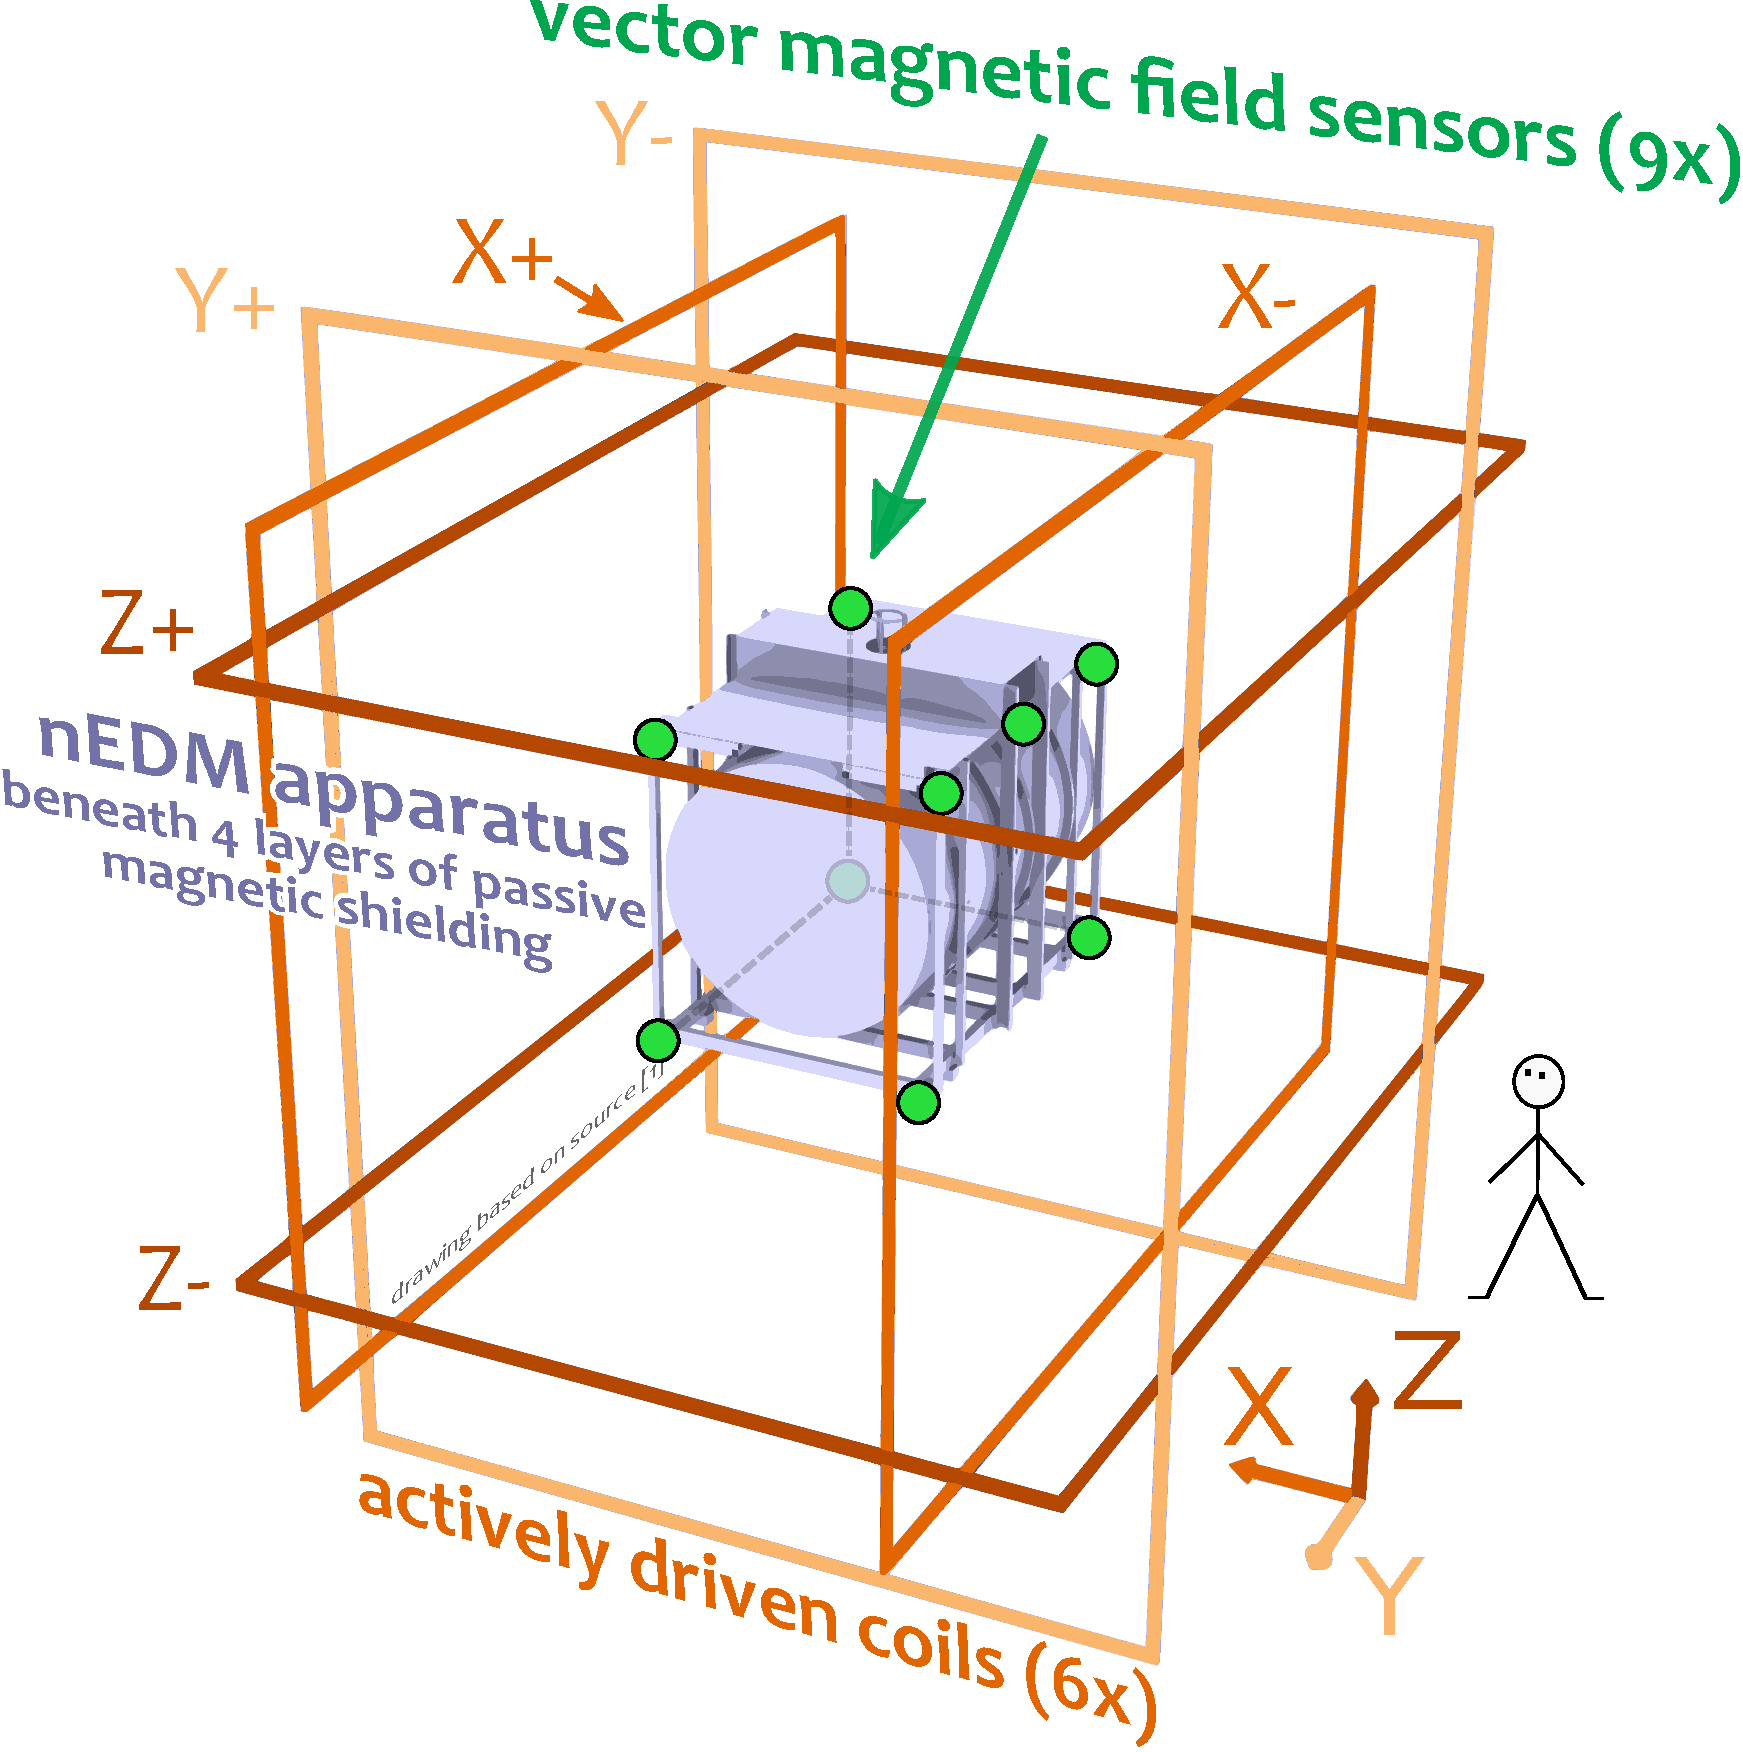
\includegraphics[width=0.8\linewidth]{gfx/nEDM_SFC/SFC_scheme.pdf}
  \caption{The nEDM at PSI active magnetic shield (SFC). The experiment, in violet, was in the middle, with nine 3-axis magnetic field sensors, depicted as green circles, attached to it. Everything was encircled by six coils (orange). Adapted from~\cite{Franke2013}.}\label{fig:sfc-scheme}
\end{figure}

Active magnetic shields follow the same principle. A volume, often called the fiducial volume, is encircled by coils. Within the volume magnetic field sensors are distributed. It is schematically presented in Fig.\,\ref{fig:sfc-scheme}, taking the PSI nEDM experiment's system as an example. The fiducial volume is filled with the violet structure in the middle (the passive shield). The green dots depict the magnetic field sensors. Around there are three orthogonal Helmholtz-like pairs of coils, depicted in shades of orange. The sensors detect the variations of the magnetic field, an appropriate counteraction is calculated and currents are applied to the coils.

\marginpar{Shielding factor, measured in \si[detect-all=true]{\decibel} is a tenth of the logarithm of the ratio of the power of the magnetic field as if it were not compensated to the compensated one.}
Active shields do not substitute passive ones.
The shielding factor of passive shields degrades for frequencies slower than \SIrange[range-phrase = --]{1}{10}{\hertz}~\cite{Brake1991,PTBroom}.
% The loss in the shielding factor can be as much as \SI{70}{\decibel} (three orders of magnitude in amplitude of the field).
At the same time active systems perform best at DC and reach up to the kilohertz regime.
The combination of the two shielding methods provides a stable magnetic field over the whole range of frequencies~\cite{Brake1991,Kelha1982,PTBroom,Voigt2013}.

Since the 1980s numerous active shields have been built~\cite{Kelha1982,Brake1991,Spemann2003,Brys2005,Kobayashi2012,Voigt2013,Afach2014}. The applications span from ion beams, through bio-magnetism, all the way to nEDM measurements, in particular the one conducted at PSI\@.

\marginpar{There was an inside joke that SFC really stands for SULTAN Field Compensation, SULTAN having been the magnet with by far the strongest influence on the magnetic field.}
\section{The nEDM at PSI SFC system}
The construction of an active shield for the nEDM measurement at PSI, called the SFC (Surrounding Field Compensation) system,
was a part of Beatrice Franke's PhD thesis~\cite{Franke2013}, later also published~\cite{Afach2014}.

% In this section the SFC system is presented, fo
% In the beginning of this chapter the most important information about the SFC system is presented, followed by a few new insights. This serves as an introduction to the original developments, to which the remaining three chapters of part II are dedicated.

The distinct feature of the PSI's SFC system was the use of a feedback matrix.
\marginpar{A matrix-based feedback was first proposed by~\cite{RetaHernandez1998}. As their proposed system did not include $\mu$-metal, they could calculate the matrix analytically.}
Consider a single coil of any shape in air. For every point in space, and for every spatial component, the magnetic field is directly proportional to the current in the coil. The SFC system had six coils and measured the field in nine points, three spatial components in each. In total there were $6 \times 27 = 162$ proportionality constants, which were gathered in the feedback matrix $M$. The matrix $M$ is a property of the active compensation system, more precisely of the geometry of the coils and sensors. It could have been calculated analytically, if not for the mu-metal shield. Ferromagnetic materials distort the magnetic field around them.
Different to similar systems~\cite{Kelha1982,Brake1991,Spemann2003,Brys2005,Kobayashi2012,Voigt2013}, which used independent feedback for each coil, the SFC system at PSI used the matrix $M$ that mixes all sensors and all coils. 
% The use of the matrix $M$ was what distinguished the PSI's SFC system from other systems~\cite{Kelha1982,Brake1991,Spemann2003,Brys2005,Kobayashi2012,Voigt2013}, which used either one component of a sensor, or a weighted combination of several components, to control one coil.

\begin{figure}
  \centering
  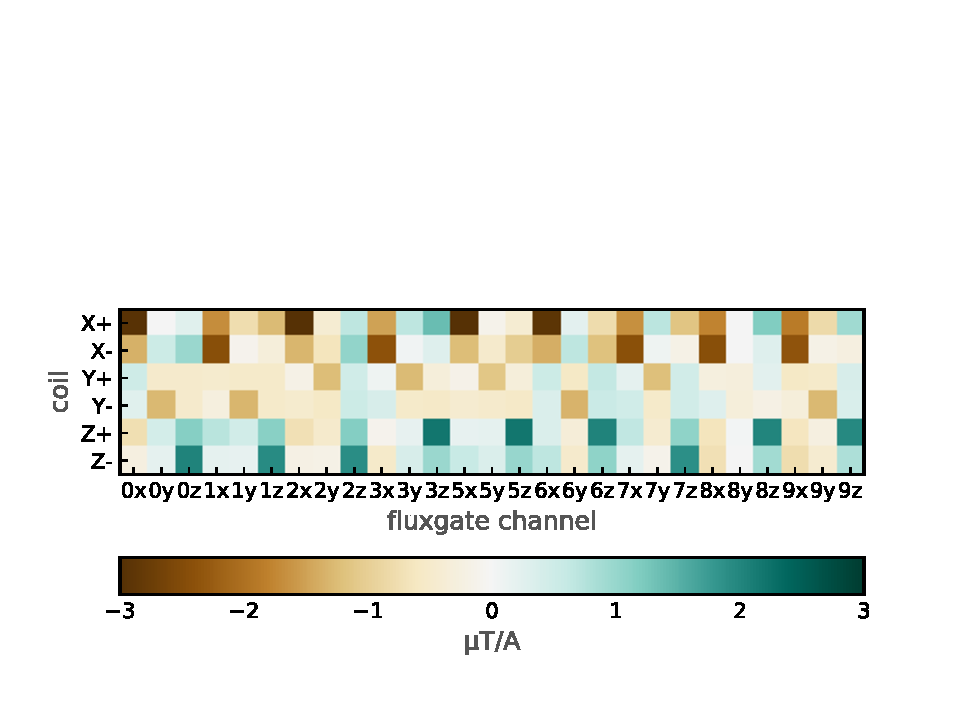
\includegraphics[width=.8\linewidth]{gfx/nEDM_SFC/nEDM_SFC_matrix.pdf}
  \caption{The SFC matrix measured by Franke on 2012--11--07~\cite{Franke2013}. For each coil (rows) and each channel of the magnetic field measurement (columns) the proportionality constant between the current in the coil and the field measured by the sensor is depicted. The coils and the sensors are labelled as in Fig.\,\ref{fig:sfc-scheme}.}\label{fig:nEDM_SFC_matrix}
\end{figure}

To measure the matrix the following procedure was used: A current in one coil was scanned in steps over the whole available range, while the field change was measured with the sensors. Then for each sensor, and each spatial component, a linear regression was performed. The slope corresponded to the proportionality constant, an element of the matrix $M$. The procedure was repeated for all coils. The matrix measured by Franke is depicted in Fig.\,\ref{fig:nEDM_SFC_matrix}.




\section{The feedback algorithm}
The PSI's SFC system followed the established norm~\cite{Kelha1982,Brake1991,Spemann2003,Brys2005} and used a PID loop to control the currents. (PI in this particular case, the derivative term was not used.) The $j$th current in the $n$th iteration was~\cite{Franke2013}:
\begin{equation}
  \label{eq:old_SFC_feedback}
  I^n_j = I^0_j +
    \underbrace{ \alpha^\mathcal{P}_j \, \Delta I^n_j }_\text{proportional term} +
    \underbrace{ \alpha^\mathcal{I}_j \, \sum_m \Delta I^m_j }_\text{integral term} \ .
\end{equation}

% $\Delta I^n_j$ is the error value in the current space. It was obtained by using the error value in the field space (the difference of the measured and target fields) and transforming it into the current space with the pseudoinverse of the matrix~\cite{Franke2013}:
$\Delta I^n_j$ is the error value. It was obtained from the deviation of the measured and target field, $\Delta B^n_{k'}$ for the $k'$th sensor, by multiplying it by the pseudoinverse of the matrix $M$, denoted $M^\dagger$~\cite{Franke2013}:
\begin{equation}
  \Delta I^n_j = \sum_{k'} M^\dagger_{jk'} \, \Delta B^n_{k'} \ .
\end{equation}

\marginpar{The SFC system, when started, was static. Then the currents could be changed manually to achieve a desired field (or chosen from a predefined set). Then the system was switched to the dynamic mode~\cite{Franke2013}.}
Besides the proportional and integral terms, the feedback formula also included the $I^0_j$ term. It may seem puzzling to give such a big of a role to particular currents that had happened to be there at the zeroth iteration. The reason behind this choice was a particular property of the SFC system: the target field was always the one measured at the moment of switching the system from the dynamic mode (feedback running) to the static one (static current output).
At that moment the error value was zero, and so was the integral term, so, according to the Eq.\,\ref{eq:old_SFC_feedback}, the output currents would immediately have switched to zero. In result the system would violently destabilise. The additional term $I^0_j$ prevented that from happening.

Here we conclude the brief description of the system and proceed to present original insights of the author.




\section{Interpretation of the feedback matrix}
There is a fundamental meaning behind the matrix $M$. The currents in the six coils can be gathered into a vector $\mathbb{I}$ in a space we call the \emph{current space}. Similarly, the 27 readouts of the magnetic field can be gathered into a vector $\mathbb{B}$ in the \emph{field space}. Then, the matrix $M$ provides the transition from the current into the field space. In particular, we have:
\begin{equation}
  \mathbb{B} = M \mathbb{I} + \mathbb{B}_\text{offset} \ .
\end{equation}
\marginpar{Finding the pseudoinverse of a matrix $A$ is equivalent to finding least-squares solution of a system of linear equations described by the matrix $A$ (although computationally more complex).}
Which is read: The measured values are a linear combination of the currents in the coils plus the ambient field.
The other direction, from the field to the current space, cannot be done exactly. Nevertheless, the optimal, in the least-squares sense, transition can be done with the use of the Moore-Penrose inverse (pseudoinverse) of the matrix $M$, denoted $M^\dagger$~\cite{penrose_1955}.
In other words, the matrix $M$ tells us what field, as measured by the sensors, a given set of currents will produce. The matrix $M^\dagger$ tells us, what currents to apply to best approximate a given field.




\section{The spectrum of the feedback matrix}
\label{sec:nedm_sfc_matrix}
The feedback matrix used during the data taking of the nEDM PSI experiment at PSI (2014--17) was the one measured by Franke (Fig.\,\ref{fig:nEDM_SFC_matrix}). The inverse of the matrix was regularised~\cite{Franke2013}. Let us now elaborate on regularisation.
% While it has been thoroughly discussed how to do the regularisation, the question of why was it needed at all was neither posed nor answered.

The feedback matrix represents coefficients in a system of linear equations that need to be solved in order to make the optimal transition from the field to the current space.
As the system of equations is over-determined, the best solution is found by the least-squares.
This is equivalent to calculating the pseudoinverse matrix. A solution can be found reliably if the system is well-defined, i.e.\ the least-squares well is steep in every direction in the parameter space.
If the well stretches, like a valley, in some directions, the solution is not globally well-defined.
Still, it may be defined up to a parameter, the one pointing along the direction of the valley.
We then speak of an ill-defined set of equations, or an ill-defined matrix.
Regularisation helps an ill-defined problem to become better defined, at the cost of the solution having larger sum of the residuals squared.

The \emph{Singular Value Decomposition} (SVD) of a real matrix $M$ is
\begin{equation}
  M = U S V^T \ , 
\end{equation}
where $U$ and $V$ are unitary, and $S$ is diagonal~\cite{Golub1965}.
The singular values lie on the diagonal of $S$, which is called the \emph{spectrum}.

\begin{figure}
  \centering
  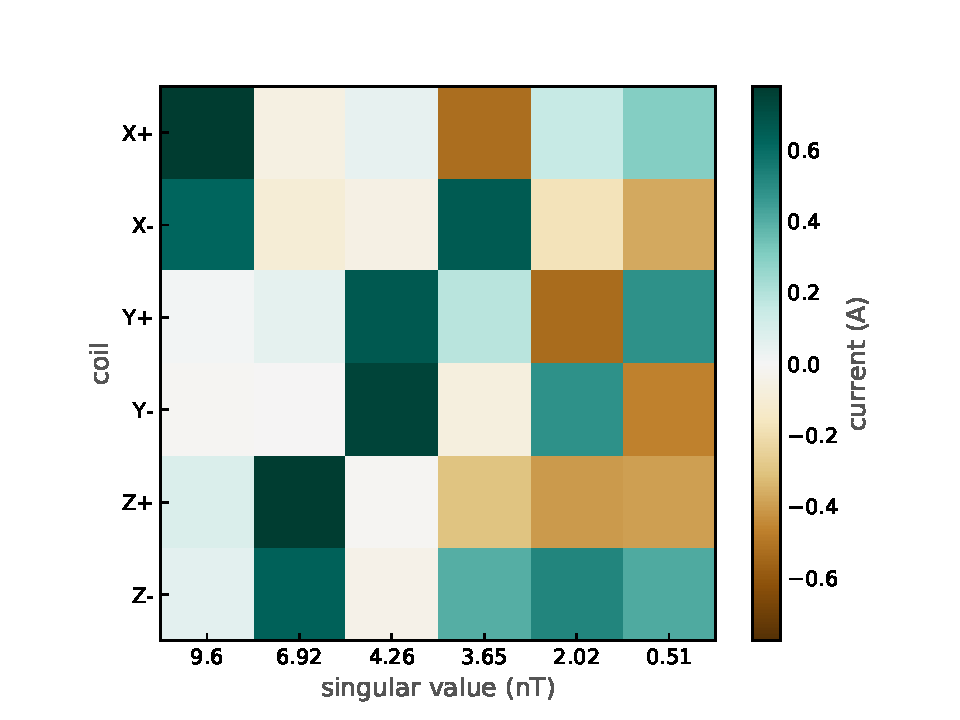
\includegraphics[width=.8\linewidth]{gfx/nEDM_SFC/coil-singular_vectors_of_the_nEDM_SFC_matrix.pdf}
  \caption{The coil-singular values of the SFC matrix.
  Columns correspond to singular combinations of the coils (labeled as in Fig.\,\ref{fig:sfc-scheme}).
  For each column the corresponding singular value is indicated.}\label{fig:nEDM_SFC_svd}
\end{figure}

The \emph{condition number} of a matrix is defined as a ratio of the extreme values of its spectrum~\cite{Regression}.
For a matrix with a flat spectrum, all singular values equal, the condition number is one.
A set of linear equations represented by such a matrix is well defined.
The more extreme values differ, the higher the condition number and the worse defined the problem is.
The effect is, that the noise in the original matrix becomes amplified by the condition number in the pseudoinverse. Figure~\ref{fig:nEDM_SFC_svd} presents the spectrum of the PSI's SFC feedback matrix.
The condition number is $9.6 / 0.51 = 18.2$.
A factor of 18 amplification of noise points to why the regularisation was necessary.

It is interesting to ask \emph{why} the system had an ill-defined feedback matrix.
A very small singular value means that there exists a coil, or a combination thereof, which has about 18 times smaller influence on the field then other ones.
In Fig.\,\ref{fig:nEDM_SFC_svd} the columns are the singular values with their corresponding coil-vectors.
The first three, starting from the left, are easiest to interpret.
Each of them is a pair of coils configured as Helmholtz-pair with roughly the same current, producing a homogeneous field in each of the spatial directions.
%The smaller singular value, or the effect on the field, in the Y direction is explained by the fact that this is the longitudinal axis of the μ-metal cylinder.
The last column has also a clear interpretation: it corresponds to all pairs configured as anti-Helmholtz---currents flowing in the opposite directions in each pair.
The magnetic field that was created by such a configuration was complicated and high-order.
The fact that this combination has so little influence on the measured field means that it hardly changes any solution for currents when added to it.
It spans a valley in the parameter space in the least-squares problem.
If not regularised, a small change in the measured field would cause a large change in the currents along the valley.
Rapid oscillations in this direction would render the system unstable.

An important observation is that the feedback matrix is defined solely by the configuration of the coils, sensors and ferromagnetic materials.
It follows that already at the design stage one can, and should, take care about the definiteness of the system.




\section{Design challenges for n2EDM}
\label{sec:n2EDM_challenges}
There was relatively a lot of space available around the passive magnetic shield of the nEDM experiment at PSI (see Fig.\,\ref{fig:sfc-scheme}).
The SFC system exploited that space by making the coils much larger than the shield.
However, the successor experiment, n2EDM, was going to have a much larger passive magnetic shield.
Spatial constraints were a major concern in the design of coils of a new active shield.

 Assume, that all there is to compensate are homogeneous fields.
 That is the zeroth order approximation concerning the space expansion of the magnetic field.
 To compensate them, a system needs to have coils that can produce a homogeneous field.
 Yet, the volume where the field of a coil system is homogeneous is limited.
 For example, in a case of a Helmholtz pair, the (linear) size of the volume where the generated field is homogeneous on a \SI{2}{\percent} level is only around \num{0.4} that of the (linear) size of the coils.
 Increasing the relative size of the homogeneous volume requires more elaborate designs~\cite{Kirschvink1992}.
 When three Helmholtz pairs are used to compensate a homogeneous change, they only do so inside this limited volume.
 Outside, the field may even be more unstable, the extreme case being right next to the coils, where the field can get arbitrarily large.
 The situation is similar for any type of field: an active shield can only stabilise the field in a limited volume.

\begin{figure}[tbh]
  \centering
  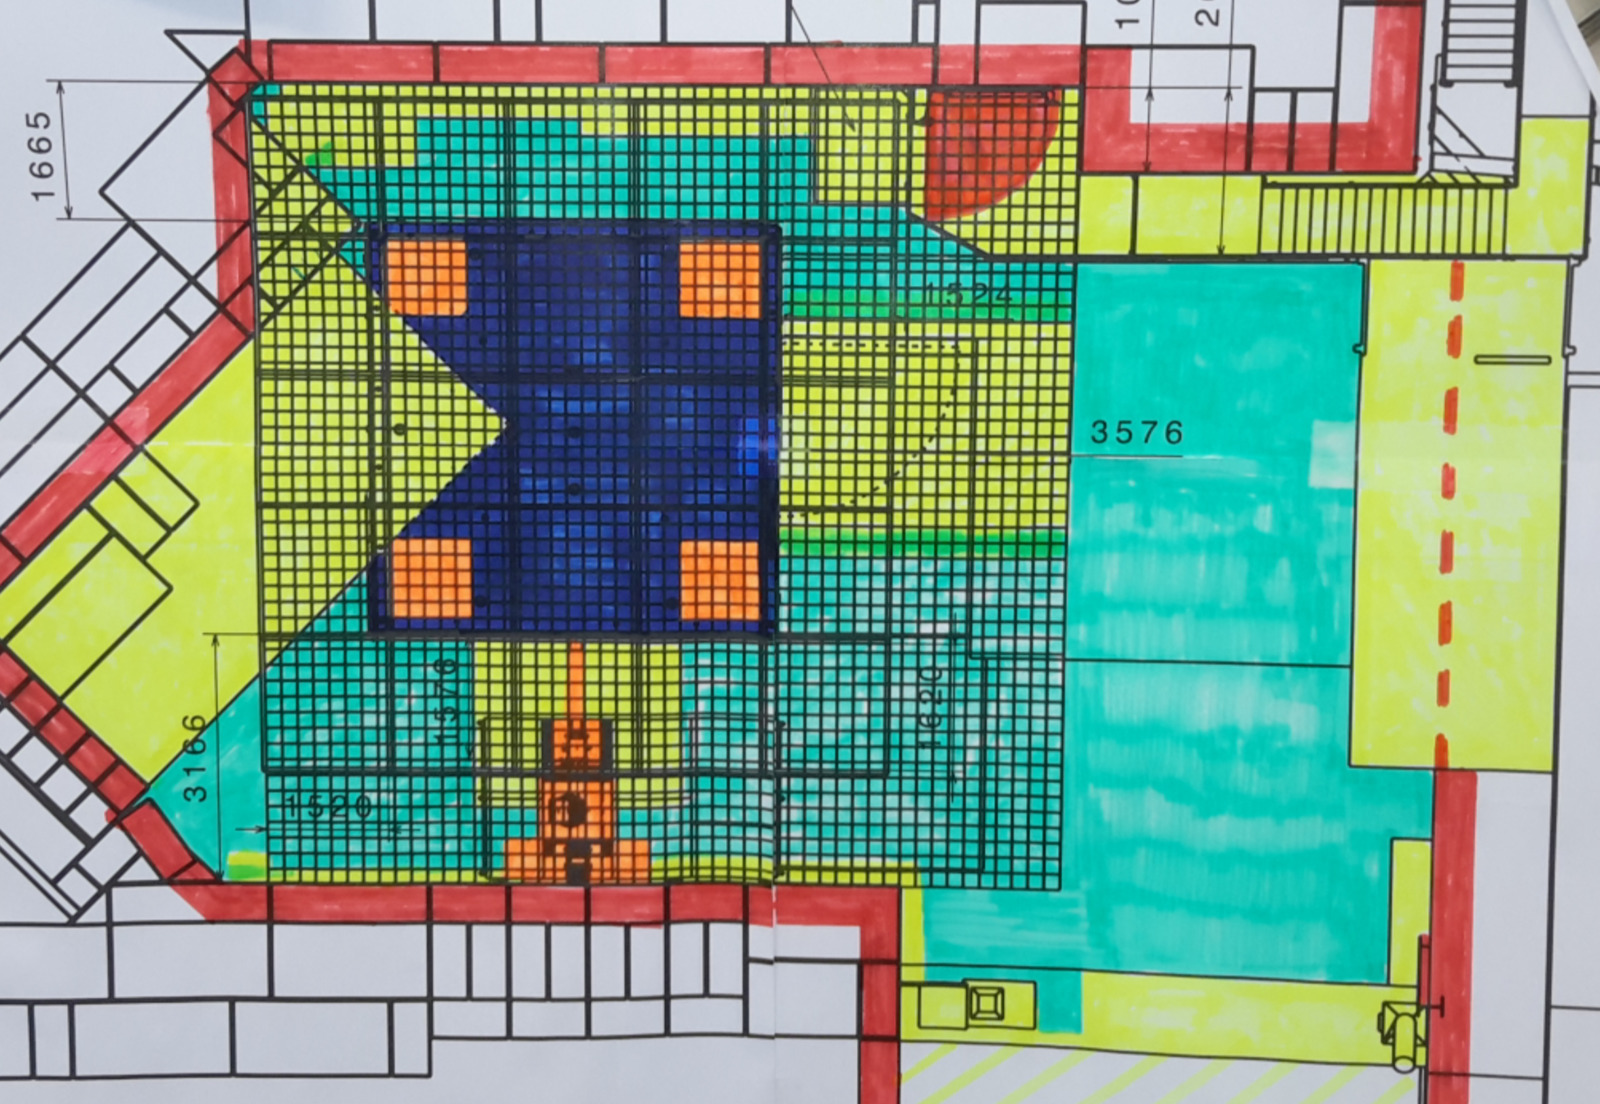
\includegraphics[width=\linewidth]{gfx/nEDM_SFC/n2EDM_SFC_situation.jpg}
  \caption{A plan by Michael Meier highlighting the potential conflicts between coils of an n2EDM active shield and other structures. The vicinity of the biological shielding (red) forced the coils to be designed relatively close to the magnetic shield (dark blue). Other bodies, like the support legs of the passive shield (orange), polarising magnet (orange) and an emergency exit from a nearby accelerator (red) gave additional constraints.}\label{fig:n2EDM_sfc_situational_plan}
\end{figure}

Figure~\ref{fig:n2EDM_sfc_situational_plan} depicts the major spatial constraints in the design of the n2EDM active shield.
Firstly, the passive shield was going to be \SI{5}{\metre} large in each direction, with the available space being $\approx \SI{7.5}{\metre}$ (a ratio of \num{0.7}).
In nEDM the shield was around \SI{2}{\meter} and the SFC coils \SIrange[range-phrase = --, range-units=single]{6}{8}{\meter} (a ratio of around \num{0.3}).
Secondly, other bodies put additional constraints (Fig.\,\ref{fig:n2EDM_sfc_situational_plan}): support legs of the passive shield, the polarising magnet and an emergency exit from a nearby cyclotron.

For the design of the n2EDM active shield it was necessary to come up with coils that could produce such a field, that they are likely to compensate, and do that in the whole volume occupied by the shield. Unfortunately, because of spatial constraints no known design could be used~\cite{Turner1986,Wong1991,Turner1993,Crozier1993,Sanchez2007,Sanchez2009}. This, together with a concern about ensuring a low condition number of the system, called for an in-depth investigation into the geometry of the future system's coils, which led to the development of a new approach to magnetic field coils design---the topic of the next chapter.

% Some came from the experimental hall itself. For example an emergency exit from a nearby accelerator and a staircase leading to it (see Fig.\,\ref{fig:n2EDM_sfc_situational_plan}). Other constraints were due to higher-priority components of the experiment itself: legs on which the shield stands, the magnet used to polarise the neutrons, the neutron detection system, and the door of the magnetic shield.

% !TEX root = ../rawlik-phd-thesis.tex
\chapter{Coil design}
\label{ch:coil_design}

In this chapter we present a new method to design a coil producing an arbitrarily shaped magnetic field. We achieve that by restricting the path of the coil's wires to a regular grid. The solution is then found by a simple least squares minimum. We discuss practical applications, in particular in an active magnetic shielding.




\section{Introduction}
\marginpar{This chapter is largely adapted from the author's publication CITE WHEN AVAILABLE}
How to design a coil, or more generally, an arrangement of coils, producing a desired magnetic field? In its simplest form this is a textbook problem (e.g.\ ex. 6.55 and 6.62 in Ref.\,\cite{Purcell}). Yet, in a general setting it is surprisingly hard and the solutions, how the wires making up the coils should be laid, complicated. The most widespread application of high-performance coils is Magnetic Resonance Imaging (MRI), where gradient coils give the possibility to produce spatial images. Already in the 1980's elaborate methods of MRI coil design have been developed. They range from optimizing positions of discrete windings, where the use is made of symmetries specific to MRI, to analytical methods yielding surface current density, which is then discretised. A general overview can be found in Ref.\,\cite{Turner1993}. Another field known for complex, precise coils is plasma confinement, in particular stellarators~\cite{Beidler1990}. There analytical solutions for the surface current density find their use, too.

Here, a new method is presented, that may not be competitive in terms of precision, but is distinct in its simplicity. Also when it comes to construction of its designs. It relies on an algebraic representation of the problem, where coil design is simplified to a simple linear least squares problem. In the method the coils are restricted to a user-defined mesh, making it easy to deal with spatial constraints.

The discussion is based on textbook linear algebra techniques, notably solving an over-determined system of linear equations, thoroughly discussed e.g.\ in Ref.\,\cite{Anton}. The main physics problem, calculating the magnetic field of coils composed of straight wire segments, is briefly discussed here. More in-depth discussions can be found, for example, in Ref.\,\cite{Griffith}. Furthermore, the implementation of the discussed problems, including examples, has been published and open-sourced~\cite{Coilsjlcode}.

We begin with a description of our model for a restricted two-dimensional case and generalize it to three dimensions. We then present how the model is used to design a coil, based on an example. Further we discuss possibilities of simplifying the solution. Another section is devoted to practical considerations, significant for the eventual construction. Finally, the application to active magnetic field shielding is considered.




\section{Coils as a linear space}
Consider all possible coils that can be constructed by laying a wire on a surface of a square. The possibilities are endless. Speaking more precisely, as the wires may be shifted by arbitrarily small distances, as they overlap and cross, the problem has inherently an infinite number of degrees of freedom. Here, an algebraic representation that reduces the number of degrees of freedom to just a few is proposed.

Start with a straight, finite wire segment spanned between points $\mathbf{x}_1$ and $\mathbf{x}_2$ (represented by vectors in an arbitrary coordinate system) and carrying current $I$, as depicted in Fig.\,\ref{fig:biot-savart}. The magnetic field it produces in the point $\mathbf{p}$ can be calculated with the use of the Biot-Savart law. Consider the vector normal to the wire through the point $\mathbf{p}$:
\begin{equation}
  \boldsymbol{\uprho} = (\mathbf{x}_1 - \mathbf{p}) - \left( \left( \mathbf{x}_1 - \mathbf{p} \right) \cdot \mathbf{n} \right)\mathbf{n} \ ,
\end{equation}
where $\mathbf{n}$ is a unit vector in the direction $\mathbf{x}_2 -\mathbf{x}_1$. The magnitude of the magnetic field in point $\mathbf{p}$ is then~\cite{Griffith}:
\begin{equation}
  \label{eq:biot_savart}
  B = \frac{\mu_0 I}{4 \pi \rho} \, \left| \sin \alpha_2 + s\, \sin \alpha_1 \right| \ ,
\end{equation}
where the angles $\alpha_i$ are not directed
\begin{equation}
  \sin \alpha_i = \frac{ \left\lVert \left( \mathbf{x}_i - \mathbf{p} \right) \times \boldsymbol{\uprho} \right\rVert }{ (x_i  - p) \rho } \ ,
\end{equation}
and $s$ is $+1$ if $\boldsymbol{\uprho}$ points onto the wire segment (between points $\mathbf{x}_1$ and $\mathbf{x}_2$) and $-1$ otherwise:
\begin{equation}
  s = \mathrm{sgn}\left( \tfrac{1}{2} \left\lVert \mathbf{x}_2 - \mathbf{x}_1 \right\rVert -
  \left\lVert \mathbf{p} + \boldsymbol{\uprho} - \tfrac{1}{2} \left( \mathbf{x}_1 + \mathbf{x}_2 \right) \right\rVert \right)
\end{equation}
\marginpar{Another formulation, with better numerical properties close to the axis of the wire, can be found in Ref.\,\cite{Hanson2002}.}
The direction of the field is given by the right-hand principle:
\begin{equation}
  \mathbf{B} = \frac{B}{\rho} \boldsymbol{\rho} \times \mathbf{n}
\end{equation}
This formulation is independent of the coordinate system (coordinate-system dependent solutions can be found e.g.\ in Ref.\,\cite{Grivich2000}).

\begin{figure}
  \centering
  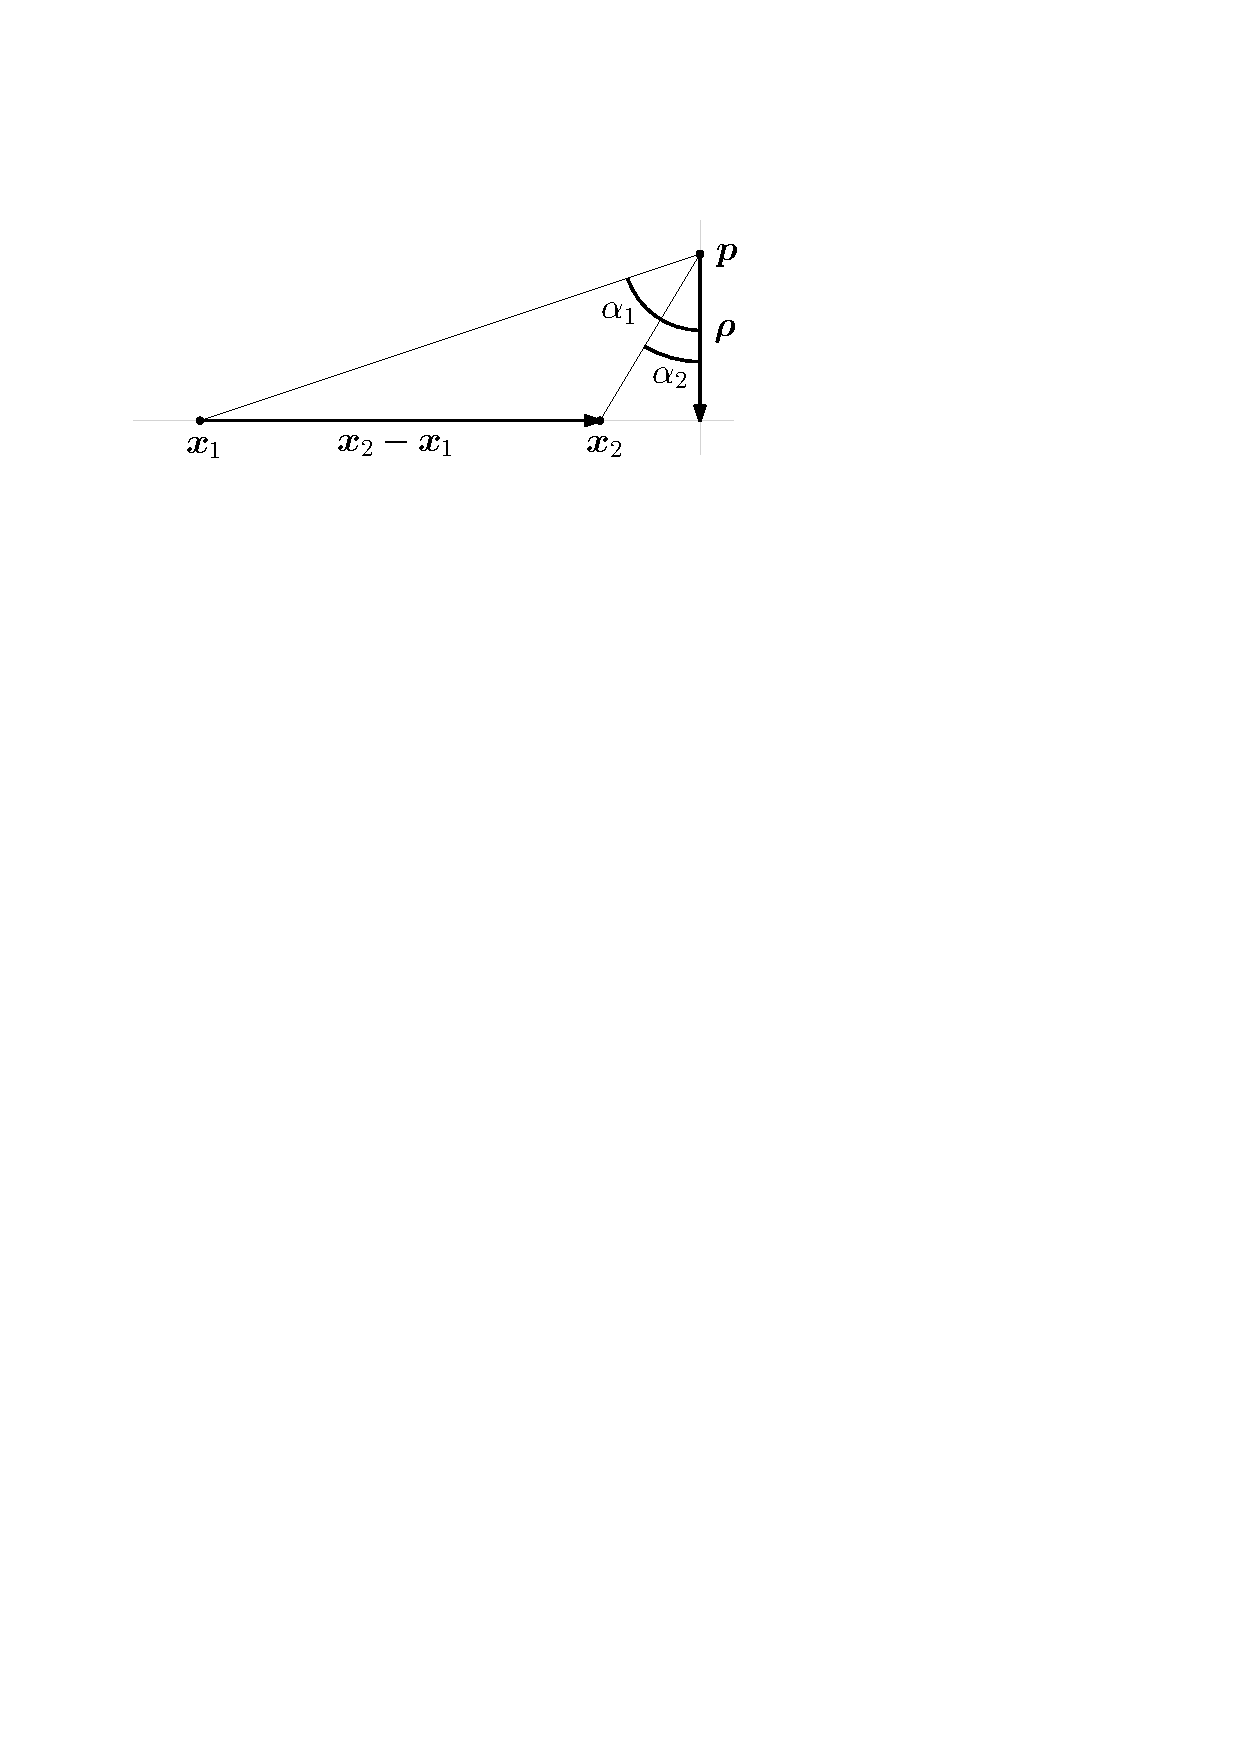
\includegraphics[width=0.6\linewidth]{gfx/coils/biot_savart.pdf}
  \caption{The setting for calculating the magnetic field produced in point $\mathbf{p}$ by a straight wire segment from $\mathbf{x}_1$ to $\mathbf{x}_2$.}\label{fig:biot-savart}
\end{figure}

Imagine four wire segments making up a square loop---a coil. It produces a certain magnetic field in the entire space $\mathbf{B}(\mathbf{x})$, given, following the superposition principle, by a sum of the fields produced by each segment of the coil.
With changing the current in the coil only one parameter of the magnetic field is altered---the magnitude, but not its shape. It can, therefore, be said that one coil spans a one-dimensional space of magnetic fields it can produce. Adding a second, different coil creates a system spanning a two-dimensional space of fields, as the magnetic field is additive. Going a step further, four square coils tiled to form a larger square form a four-dimensional space, as shown in Fig.\,\ref{fig:coils_tile_basis}. Any coil restricted to the $2 \times 2$ grid can be represented in the base of the four tile-coils.

The range of magnetic field reachable by coils restricted to a grid is a subset of all possible fields that can be created with coils constructed on the square's surface. The size of the subset is controlled by $N$, the number of tile-coils forming the grid.
In this system a coil is fully described by a vector of $N$ currents, one in each of the tile-coils, denoted by $\mathbb{I}$. The problem of coil design is thereby simplified to finding a vector $\mathbb{I}$.

\begin{figure}
  \centering
  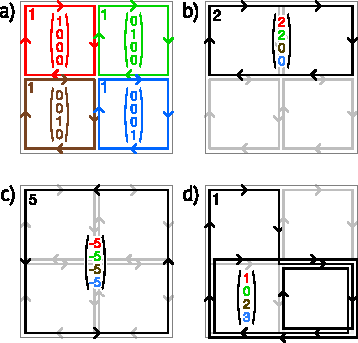
\includegraphics[width=0.6\linewidth]{gfx/coils/tile_basis.pdf}
  \caption{a) A basis of four tile coils on a flat square. Any coil which has its wires restricted to lie on the $2 \times 2$ grid can be represented as a linear combination of the four base tile coils. b, c, d) Three coils are presented together with their explicit coordinates in the basis.}\label{fig:coils_tile_basis}
\end{figure}

Generalisation onto a cube is simple. A cube is made up of six square faces. Interestingly, for the assembly in the three-dimensional space one degree of freedom is lost.  Figure~\ref{fig:coils_tile_kernel} illustrates, in the simplest case $N = 6$, a configuration in which finite currents in all six coils cancel and no magnetic field is produced. Such a combination of currents can be added to any solution with no effect on the produced field. Effectively, the space of the fields they can produce has dimension five (i.e.\ $N-1$). In other words, the mapping of $\mathbb{I}$ onto fields $\mathbf{B}(\mathbf{x})$ has in this case a one-dimensional kernel. This fact is of importance when it comes to numerically solving the system.

\begin{figure}
  \centering
  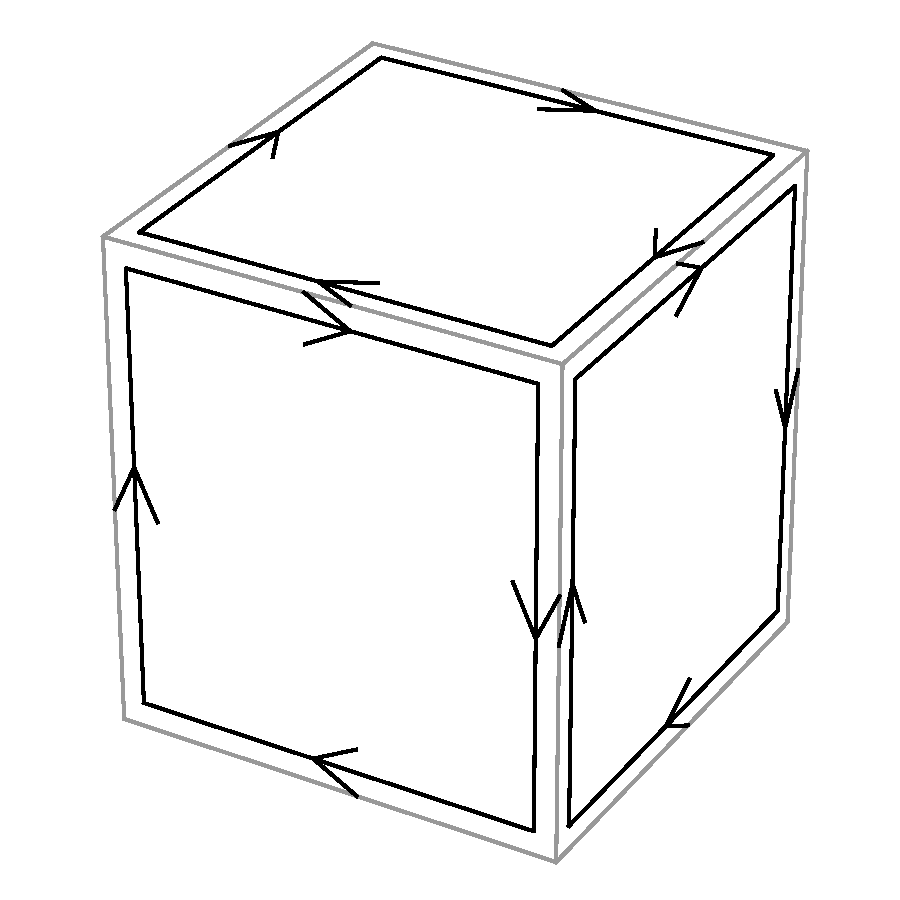
\includegraphics[width=0.5\linewidth]{gfx/coils/tile_kernel2.pdf}
  \caption{An arrangement of $N = 6$ tile coils on a cube which produces no magnetic field. The currents in the tiles are equal and flow in the directions as indicated. The currents on the invisible faces are analogous to the ones seen in front. For clarity, the coils are depicted slightly smaller; in the model the currents are identical with the edges of the cube.}\label{fig:coils_tile_kernel}
\end{figure}

This is the foundation of the method. The restriction to a grid on a cuboid enables all coils in the restricted space to be described by a vector of $N$ numbers.




\section{Coil design}
In the problem of coil design a coil is sought, or an arrangement of coils, which best approximates a given field in a certain volume. The volume we shall call \emph{the volume of interest}. Rather than considering the whole volume, an ensemble of $m$ points of interest on its surface is picked (the surface is sufficient because $\nabla \cdot \mathbf{B} = 0$). Henceforth, the magnetic field $\mathbf{B}(\mathbf{x})$ only at these points is considered. The values $\mathbf{B}(\mathbf{x}_i)$ for $i = 1 .. m$ are gathered into a vector of dimension $3m$ ($B_x$, $B_y$ and $B_z$ in each point), which we shall denote $\mathbb{B}$.

As mentioned before, the magnetic field produced by a coil at any given point in space is proportional to the current in this coil. With many coils present it is a linear combination of the currents of all coils in the system. In an absence of an external magnetic field the system of $N$ tiles and $m$ points of interest is thus described by a simple linear equation:
\begin{equation}
  \label{eq:matrix}
  \mathbb{B} = M \, \mathbb{I}\ ,
\end{equation}
where $M \in \mathbb{R}^{3 m} \times \mathbb{R}^{N}$ is a matrix of proportionality constants. For example, the element $M_{(5, 2)}$ is the proportionality constant between the current in the second of $N$ coils and the magnetic field in the $y$ direction in the second of $m$ points of interest, $B_y(\mathbf{x}_2)$. The matrix $M$ can be calculated analytically using the Biot-Savart law.

Equation~\ref{eq:matrix}, for $3m > N - 1$, is an over-determined system of linear equations, $\mathbb{I}$ being the vector of unknowns. The optimal least-squares solution $\mathbb{I}_0$ to produce a $\mathbf{B}_0(\mathbf{x})$ in the volume of interest is
\begin{equation}
  \label{eq:requirement}
  % M \, \mathbb{I} \stackrel{!}{=} \mathbb{B}_0
  \mathbb{I}_0 = \arg\,\min_{\mathbb{I}} {\left( M \mathbb{I} - \mathbb{B}_0 \right)}^2 \ .
\end{equation}
The optimal solution can be calculated with the normal equation~\cite{Anton}:
\begin{equation}
  \mathbb{I}_0 = {\left( M^\mathrm{T} M \right)}^{-1} M^\mathrm{T} \mathbb{B}_0 \ ,
\end{equation}
\marginpar{Least-squares is solved with a backslash operator in MATLAB-like languages:\\
\texttt{I0 = M \textbackslash{} B0.}}
but the problem is typically solved numerically. The majority of numerical software packages use the QR decomposition (a product of an orthogonal and upper-triangular matrix) of the matrix $M$, which is more numerically stable when compared to the normal equation.

Depending on the properties of $M$ the optimum may be multidimensional. In particular, as already mentioned, an arrangement of coils on a cube has a one-dimensional kernel, which will always cause the optimum to be at least one-dimensional. In these cases, we will call $\mathbb{I}_0$ the unique least-norm solution, which minimizes the total current in the system. $\mathbb{I}_0$ is the vector of the optimal currents in the tile arrangement of coils for approximating $\mathbf{B}_0(\mathbf{x})$ in the volume of interest.

\begin{figure}
  \centering
  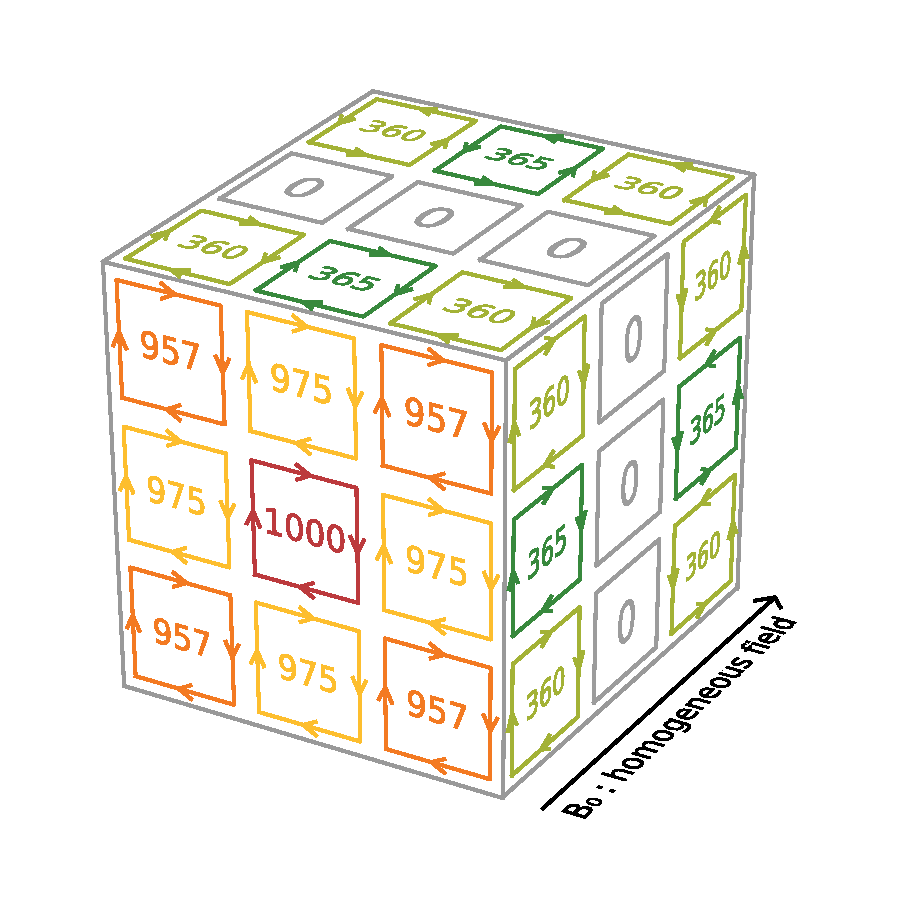
\includegraphics[width=\linewidth]{gfx/coils/homogeneous_tiles_norm_1000.pdf}
  \caption{A solution of a tile system with $N = 6 \times (3 \times 3)$ tiles on a unit cube for a homogeneous field. The volume of interest is a cube with side length \num{0.75}, centered inside the unit cube. Numbers indicate currents in the tile coils in arbitrary units. The currents are normalized so that the highest is \num{1000}. For clarity, the coils are depicted slightly smaller; in the model their edges overlap. The currents on the three invisible faces are by symmetry analogous to the visible ones.}\label{fig:homogeneous_tiles}
\end{figure}

\begin{figure*}
  \centering
  \subfloat{\label{fig:homogeneous_performance_a}
    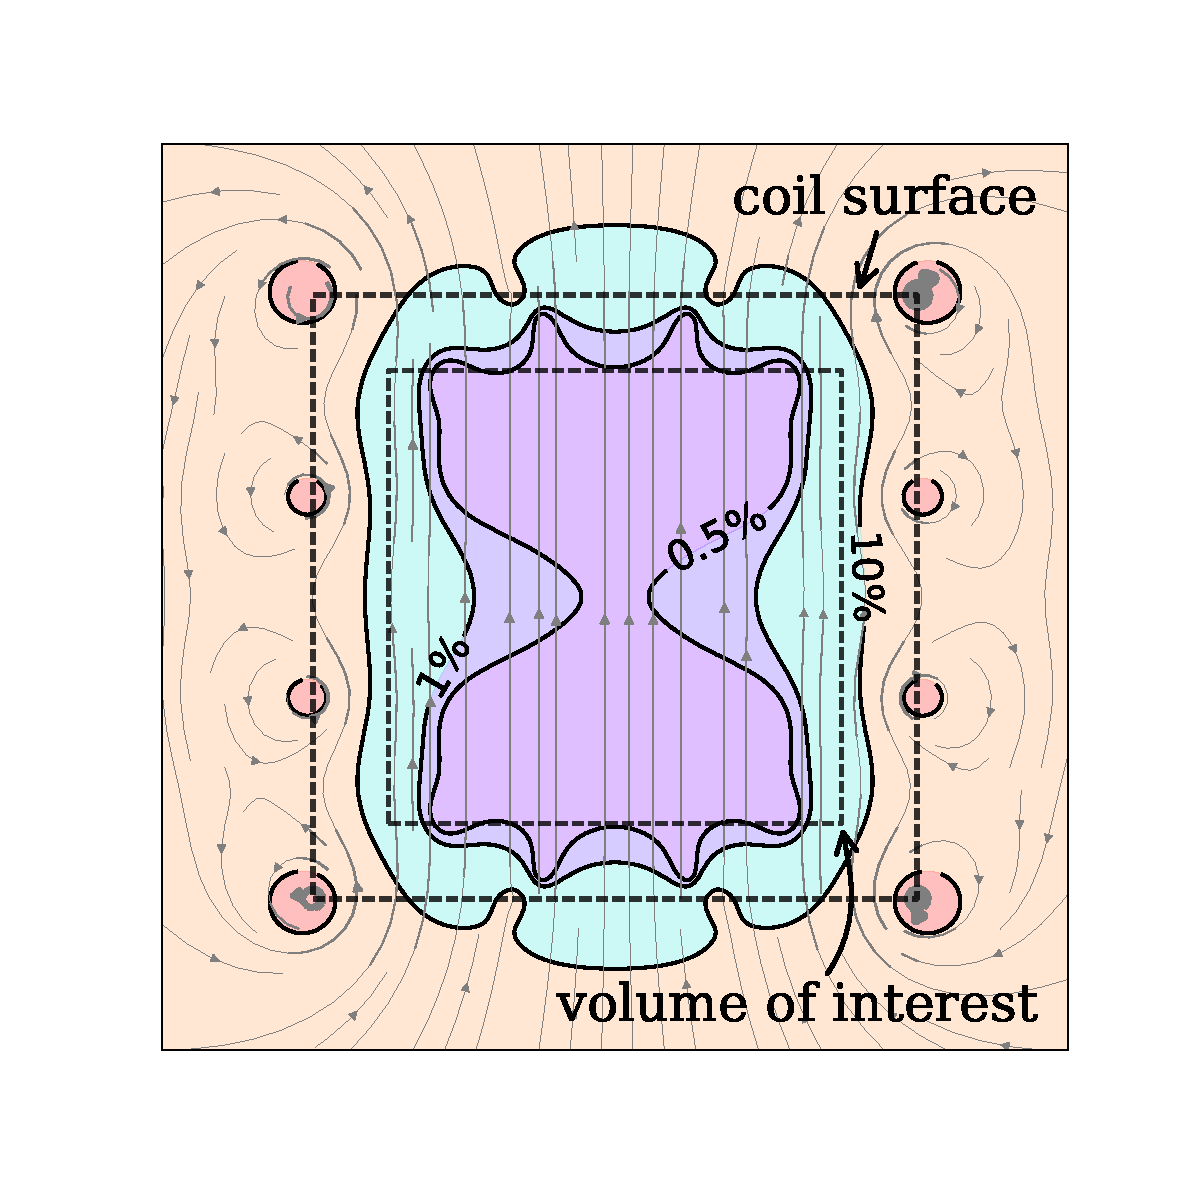
\includegraphics[width=.49\linewidth]{gfx/coils/homogeneous_performance.pdf}}
  \subfloat{\label{fig:homogeneous_performance_b}
    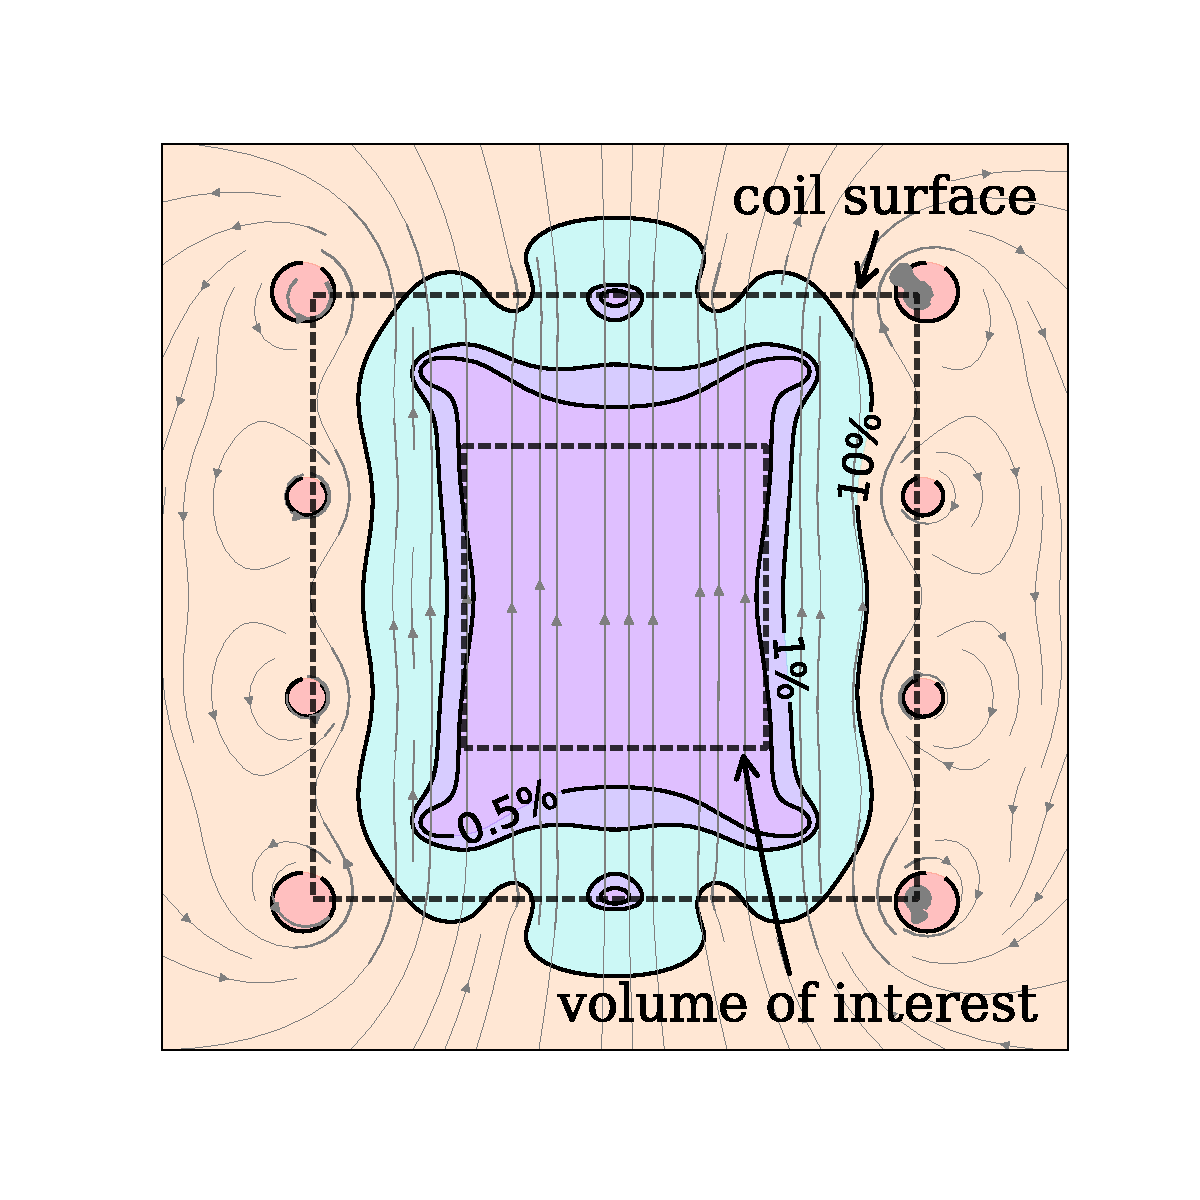
\includegraphics[width=.49\linewidth]{gfx/coils/homogeneous_performance_smaller_volume.pdf}}
  \caption{Magnetic field produced by a coil designed for a homogeneous field, with $N = 6 \times (3 \times 3)$ tiles on a unit cube. The field lines are depicted in grey. Contours show boundaries of \num{0.5}, \num{1} and \SI{10}{\percent} magnitude deviation from an ideal homogeneous field. Horizontal cross sections in the middle-height plane are shown. Two designs are presented. Left-hand side: the volume of interest is a cube with side length \num{0.75} (the individual tile coil currents are depicted in Fig.\,\ref{fig:homogeneous_tiles}), right-hand side: the size of volume of interest is reduced to \num{0.5}.}\label{fig:homogeneous_performance}
\end{figure*}

Let us consider an example of a coil design on a unit cube with the number of tiles $N = 6 \times (3 \times 3)$ (see Fig.\,\ref{fig:homogeneous_tiles}). As the volume of interest we pick a cube, centered with the unit one, with side length \num{0.75} (with a regular mesh of $10 \times 10$ points on each face, a total of $m = 488$ points of interest). For the sake of simplicity we design a coil for a homogeneous field along an axis of the cube. The solution of Eq.\,\ref{eq:requirement}, $\mathbb{I}_0$, directly gives the currents in each tile. They are graphically depicted in Fig.\,\ref{fig:homogeneous_tiles}. Note, that many currents almost cancel each other, in particular those along horizontal edges. The magnetic field produced by the solution is shown on the left-hand side in Fig.\,\ref{fig:homogeneous_performance}, as a horizontal cut along the central plane. Contours show the relative deviation from the homogeneous field. Inside the volume of interest (dashed line), the design goal of a homogeneous field is reproduced with few per cent accuracy. The solution, and thus the contours too, depend on the choice of the volume of interest. In general, the further away the volume of interest is from the coils, the better the accuracy. If the side length of the volume of interest is decreased to \num{0.5}, the accuracy improves to \SI{1}{\percent}, as shown on the right-hand side in Fig.\,\ref{fig:homogeneous_performance}. The optimal solution, and thereby the shape of the precision contours, change. Naturally, the accuracy of the field reproduction can also be improved by increasing the number of tiles.




\section{Simplification of the tile system}
The tile system may find an interesting practical application. Once independently controllable tiles have been built, it can be used to produce an arbitrary field. However, building many independently driven coils is a high price to pay for producing only one field. Additionally, each edge is shared between two tiles, and the effective current is the sum of two. They may add either constructively or destructively. If the given solution is dominated by subtraction of large currents, a lot of power is unnecessarily dissipated in the system. It turns out, that both problems can be solved by simplifying the tile solution.

\begin{figure*}
  \centering
  \subfloat{\label{fig:coils_dipole_3d_1}
    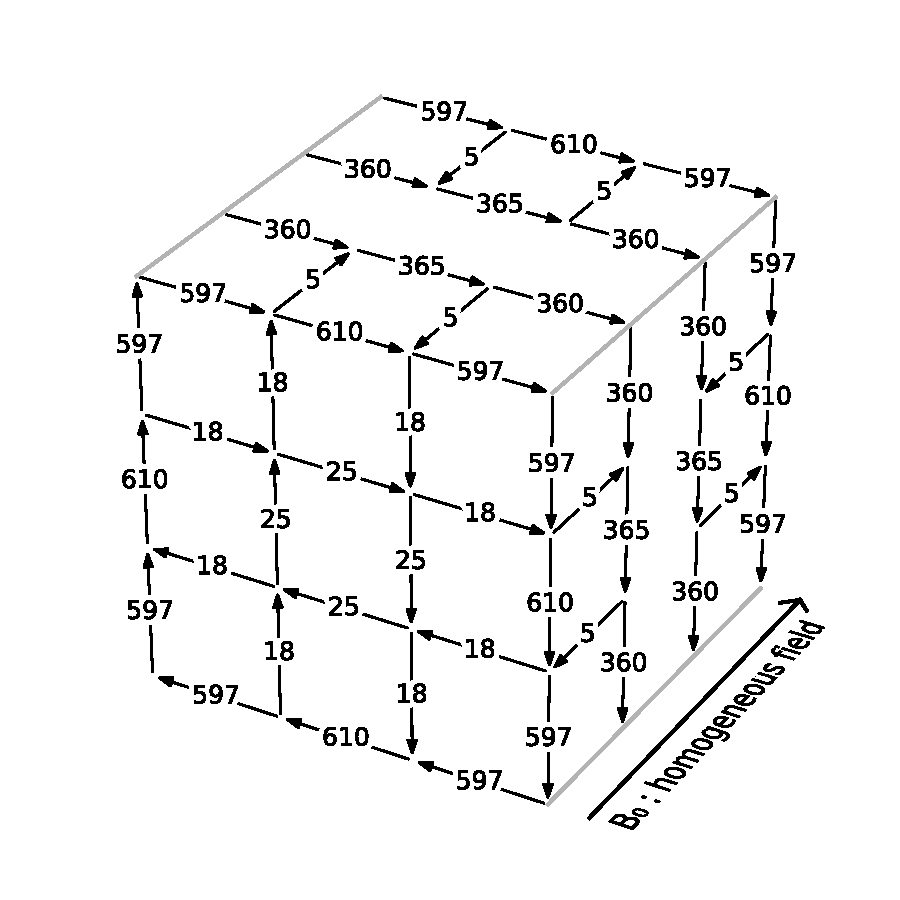
\includegraphics[width=.49\linewidth]{gfx/coils/algorithm_net_1.pdf}}
  \subfloat{\label{fig:coils_dipole_section_0}
    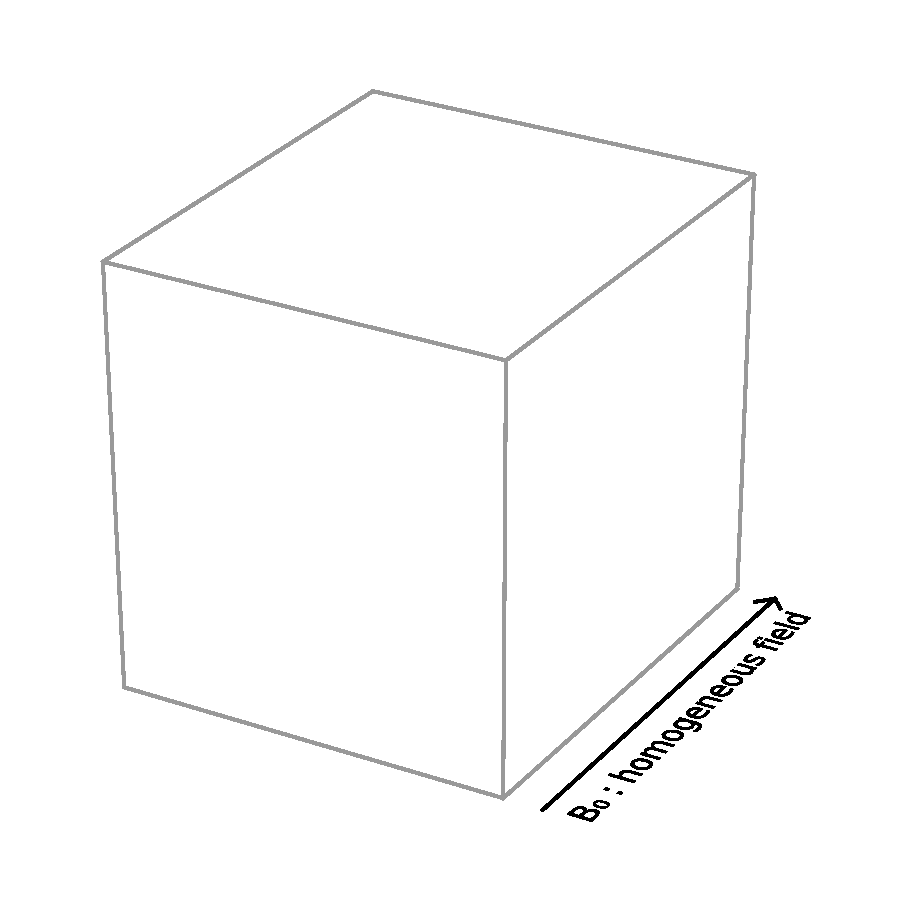
\includegraphics[width=.49\linewidth]{gfx/coils/algorithm_simplified_0.pdf}}
  \\
  \subfloat{\label{fig:coils_dipole_3d_3}
    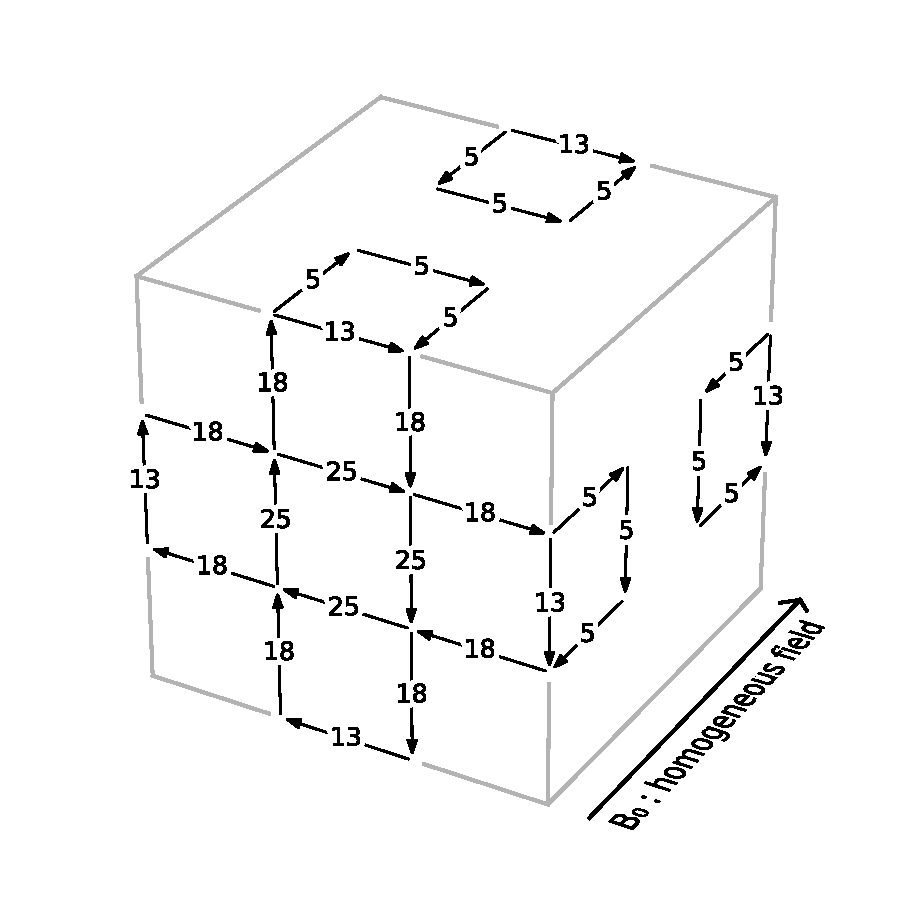
\includegraphics[width=.49\linewidth]{gfx/coils/algorithm_net_3.pdf}}
  \subfloat{\label{fig:coils_dipole_section_2}
    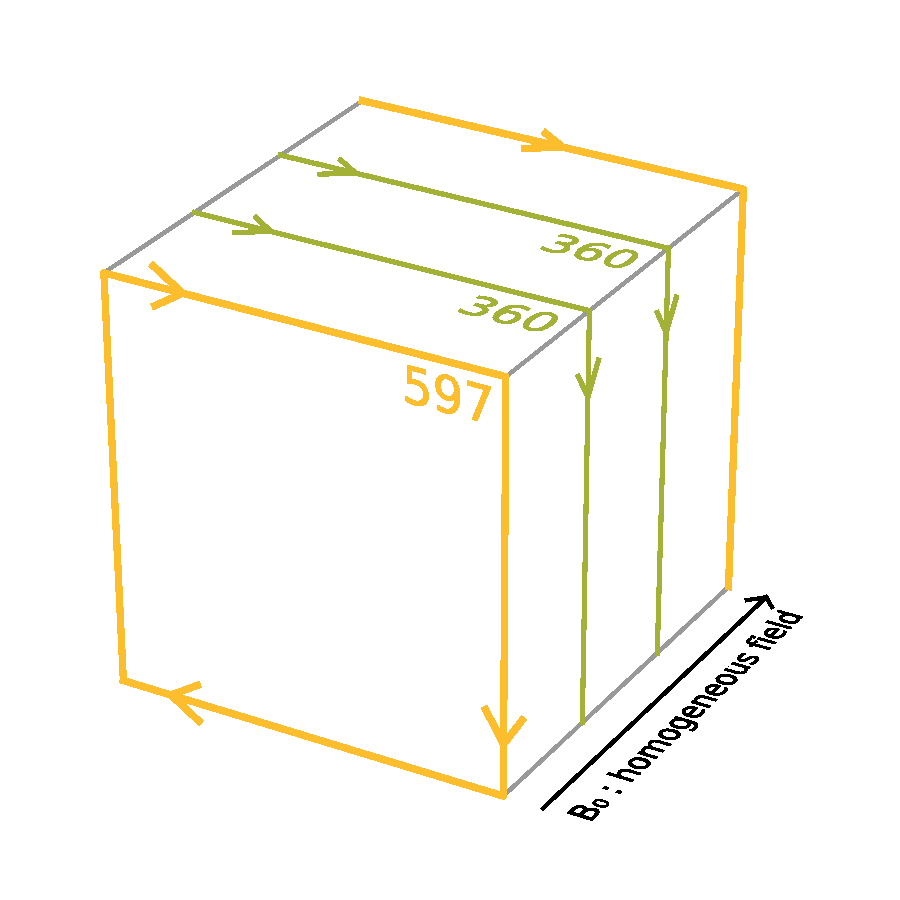
\includegraphics[width=.49\linewidth]{gfx/coils/algorithm_simplified_2.pdf}}
  \\
  \subfloat{\label{fig:coils_dipole_3d_5}
    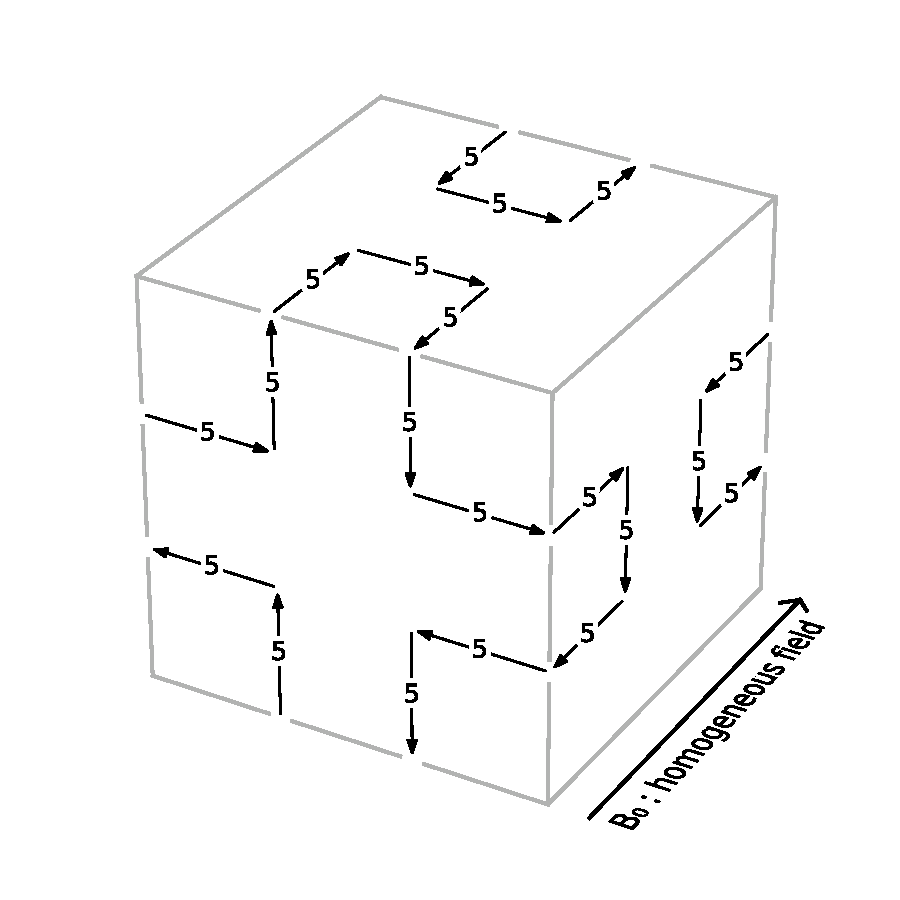
\includegraphics[width=.49\linewidth]{gfx/coils/algorithm_net_5.pdf}}
  \subfloat{\label{fig:coils_dipole_section_4}
    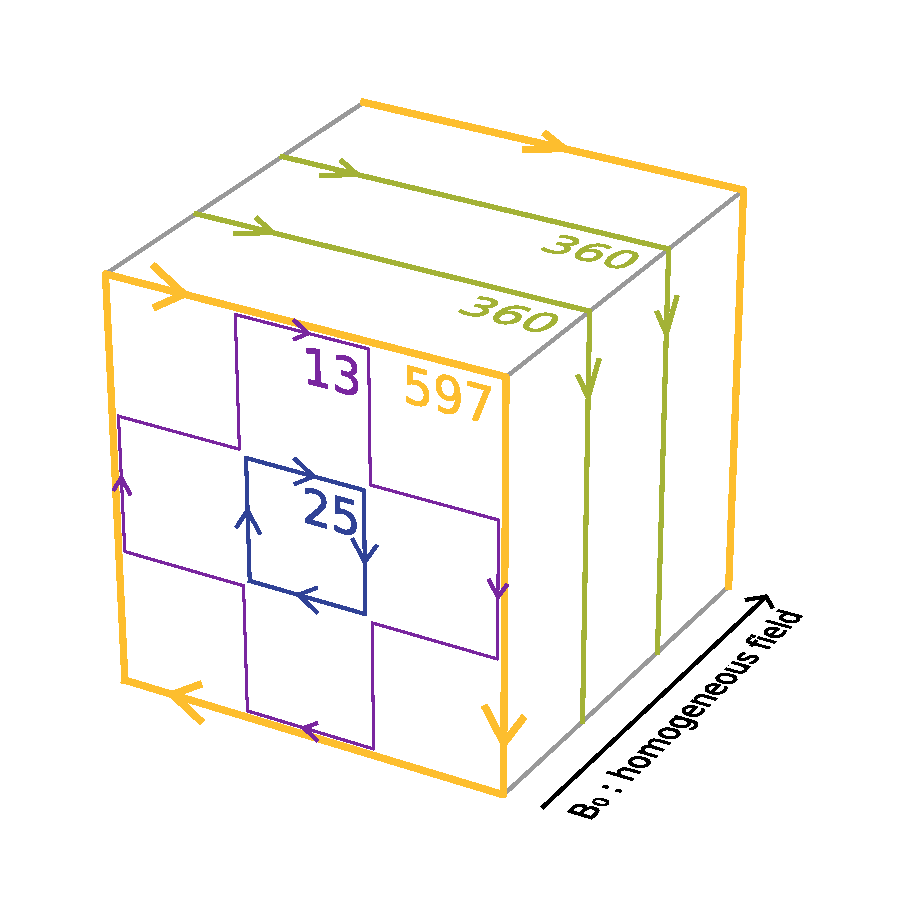
\includegraphics[width=.49\linewidth]{gfx/coils/algorithm_simplified_4.pdf}}
  \caption{Following the algorithm to simplify a coil. The left column shows the net of a current with the total current along edges of tiles. In each iteration the loop with the highest current is found and transferred onto the simplified solution, shown in the right column. We show iterations, from top: zeroth, fourth and eighth.}\label{fig:simplification_algorithm}
\end{figure*}

\begin{figure}
  \centering
  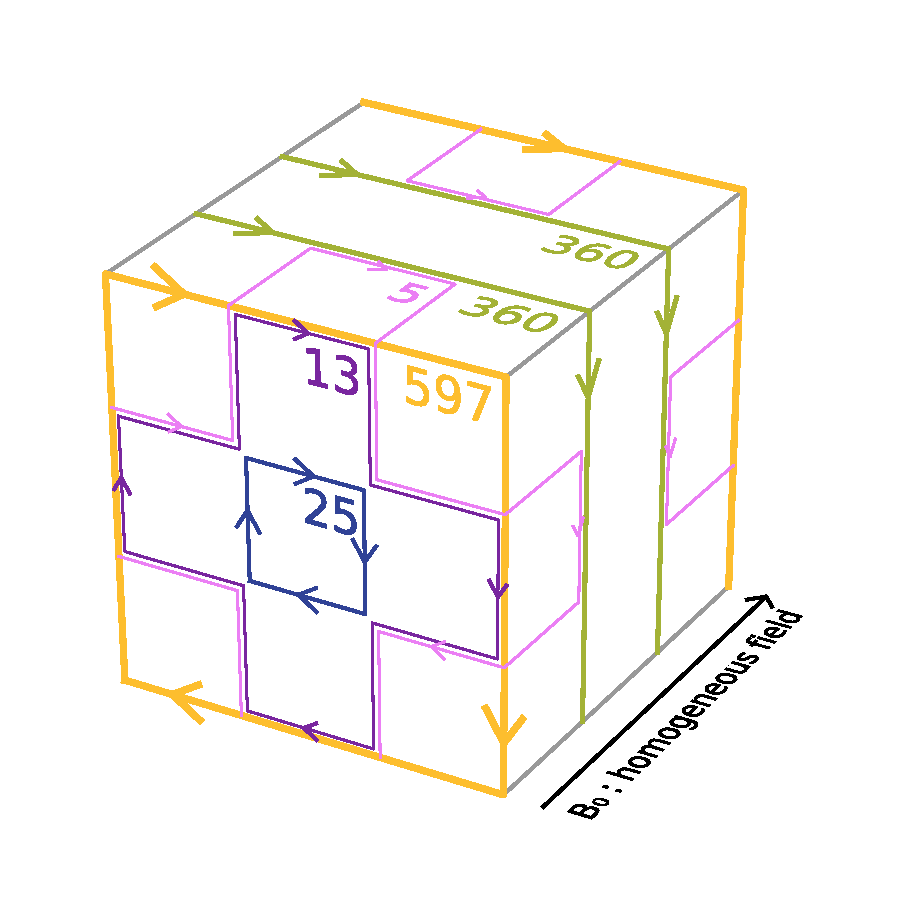
\includegraphics[width=\linewidth]{gfx/coils/algorithm_simplified_5.pdf}
  \caption{The coil designed for a homogeneous field, with $N = 6 \times (3 \times 3)$ tiles (Fig.\,\ref{fig:homogeneous_tiles}), simplified by adding the currents along each edge and decomposing into current loops.}\label{fig:homogeneous_coils}
\end{figure}

One starts by adding the currents of the adjacent tiles and assigning the sum to each common edge. The result is a complicated net of currents (upper left corner of Fig.\,\ref{fig:simplification_algorithm}). Still, each node fulfills Kirchhoff's laws. The net can then be decomposed into simple current loops by following the algorithm: First find in the net the loop with the highest current. In the example it is either of the ``\num{597}'' loops on the front and back faces. This loop will make the first one in the simplified solution (it can be seen in the middle of the right column in Fig.\,\ref{fig:simplification_algorithm}, together with the next three loops). Then subtract from the net the current of the first loop along its edges (the net that remains after subtracting the first four loops is depicted in the middle of the left column in Fig.\,\ref{fig:simplification_algorithm}). Finally, continue to find the loop with the highest current in the modified net, which will give the next loop and repeat until the current net is empty. The net remaining after eight loops are found is depicted in the bottom row of Fig.\,\ref{fig:simplification_algorithm}, next to the first eight loops. The final simplified solution is shown in Fig.\,\ref{fig:homogeneous_coils}. The currents in the simplified coil system are much smaller, the highest being \num{597} instead of \num{1000} and they always add constructively. Also, the number of separate loops is decreased from \num{42} to \num{10}. Still, the total current along each edge of a tile is exactly the same as in the tile configuration.

We conclude here our method of coil design. The simplified arrangement of coils is the optimal one, given the grid restriction, for approximating the magnetic field in the volume of interest. We continue to consider practical aspects, relevant for constructing the designs of the new method.




\section{Practical considerations}
The primary practical advantage of the new design method is that the coils are constrained to a predefined grid. This is contrary to other methods of coil design, where the position of the wires is the output of the procedure~\cite{Turner1993, Beidler1990}. This may prove useful in applications with spatial constraints. Typically, coils need to be incorporated into a setup in which other components penetrate the surface on which the wires are laid. In the new method it is possible to simply define the grid so that no collisions occur. Although the simple examples presented before used regular grids, we have not used symmetries to solve the problem. When many coils are designed and built, for instance to produce homogeneous magnetic fields in each of the three dimensions, they can all share the same grid. The grid can, for example, be constructed out of cable channels into which the wires are laid.

A limitation associated with the finite size of the channels is the strength of the magnetic field that can be created, which, for given available power, is limited by the thickness of the wire. At the same time, the finite size of the cable channels can be neglected in the calculations only as long as it is small compared to the distance between the coils and the volume of interest. Using an enameled wire, rather than a standard, PVC-insulated cable, can reduce the overall thickness.

In the proposed solution in order to produce the desired field one still needs a system of several coils, even in the simplified solution. The more complicated the goal field, and the more tiles, the more different currents are needed across the individual loops, which quickly becomes impractical. There are several ways to tackle the problem.

The first way is to use only one current and adjust by varying the number of windings. In the example, when one decides for \num{60} windings as the maximum, then the nominal current that would flow through the wire is $\mathrm{round}(597 / 60) = 10$. The \num{597}, \num{360}, \num{25}, \num{13} and \num{5} would be created with \num{60}, \num{36}, \num{3}, \num{1} and \num{1} windings, respectively. A discretisation error of $10 / 597 = \SI{1.7}{\percent}$ is of the same order as the accuracy of the solution in representing the field (see Fig.\,\ref{fig:homogeneous_performance}). For more precise designs the numbers of windings get larger, which is troublesome to construct and causes the coils to have larger inductances.

A second way is to use a current divider. That is to connect the different loops in parallel, each with an appropriately chosen resistance in series. This way the ratios between the currents in each loop can be tuned precisely. However, a practical realization will most likely involve routing all loops out of the system where the current divider is installed. For more complicated coil systems with tens of different currents this may be impractical.

Yet another way is to split the loops into decades of currents.
In the coil we use as an example, the currents \num{597}, \num{360}, \num{13}, \num{7}, \num{5} (in arbitrary units) may be constructed from a set of wires with three relative currents of \num{100}, \num{10} and \num{1}:
\marginpar{A base different than 10 can be used, too.}
\begin{align*}
  597 & = 5 \times 100 + 9 \times 10 + 7 \times 1 \\
  360 & = 3 \times 100 + 6 \times 10 + 0 \times 1 \\
  13 & = 0 \times 100 + 1 \times 10 + 3 \times 1 \\
  7 & = 0 \times 100 + 0 \times 10 + 7 \times 1 \\
  5 & = 0 \times 100 + 0 \times 10 + 5 \times 1 \ .
\end{align*}
In this way accuracy better than \SI{1}{\percent} in reproducing the solution can be reached with only three different currents to control, even for complicated designs. Those can be either separately controlled or split with a current divider.

No claim is made as to superiority of one of the three above solutions over the other two. It is up to the particular application which is the best suited one.




\section{Application to active magnetic field shielding}
Using the method presented here to design coils of an active magnetic shield  offers improvements in two areas. Firstly, the size of the coils could be decreased, or the size of the experimental set-up increased, without loss of performance. Better homogeneity in a given volume can always be achieved by choosing a denser gird. Given the tight spatial constraints this was a crucial development for the design of the n2EDM's active shield.

\begin{table}
  \centering
  \begin{tabular}{c|ccc}
    n & $\mathbf{P}_n^x(\mathbf{r})$ & $P_n^y(\mathbf{r})$ & $P_n^y(\mathbf{r})$ \\ \midrule
    1 & 1 & 0 & 0 \\
    2 & 0 & 1 & 0 \\
    3 & 0 & 0 & 1 \\
    \midrule
    4 & $x$ &  0  & $-z$ \\
    5 & $y$ & $x$ &   0  \\
    6 &  0  & $y$ & $-z$ \\
    7 & $z$ &  0  & $ x$ \\
    8 &  0  & $z$ & $-y$ \\
  \end{tabular}
  \caption{Cartesian harmonic polynomials.}\label{tab:coils_cartesian_harmonics}
\end{table}

Secondly, the method allows to construct a coil for any field. In particular, one may choose to construct coils that produce fields orthogonal to one another. 
% (as $\mathbb{R}^3 \rightarrow \mathbb{R}^3$ functions).
This makes an active shielding system significantly easier to control~\cite{MRM:MRM1910010107} and avoids a potential problem of the high condition number due to very-high-order fields produced by pathological combinations of coils (recall the discussion in Sec.\,\ref{sec:nedm_sfc_matrix}). One of the possible orthogonal decompositions of the field is the one into \emph{cartesian harmonic polynomials}~\cite{Franke2013}:
\begin{equation}
  \mathbf{B}(\mathbf{r}) = \sum_{n}\,H_n \mathbf{P}_n(\mathbf{r}) \ ,
\end{equation}
where $H_n$ are the expansion coefficients, and $\mathbf{P}_n(\mathbf{r})$ are the cartesian harmonic polynomials, the first eight of which are listed in Table~\ref{tab:coils_cartesian_harmonics}. Each term satisfies by itself the Maxwell's equations. The first three terms are homogeneous fields, the next five are the five independent linear gradients. Further ones correspond to higher-order gradients.

\begin{figure*}
  \centering
  \subfloat{\label{fig:coils_dipole_3d}
    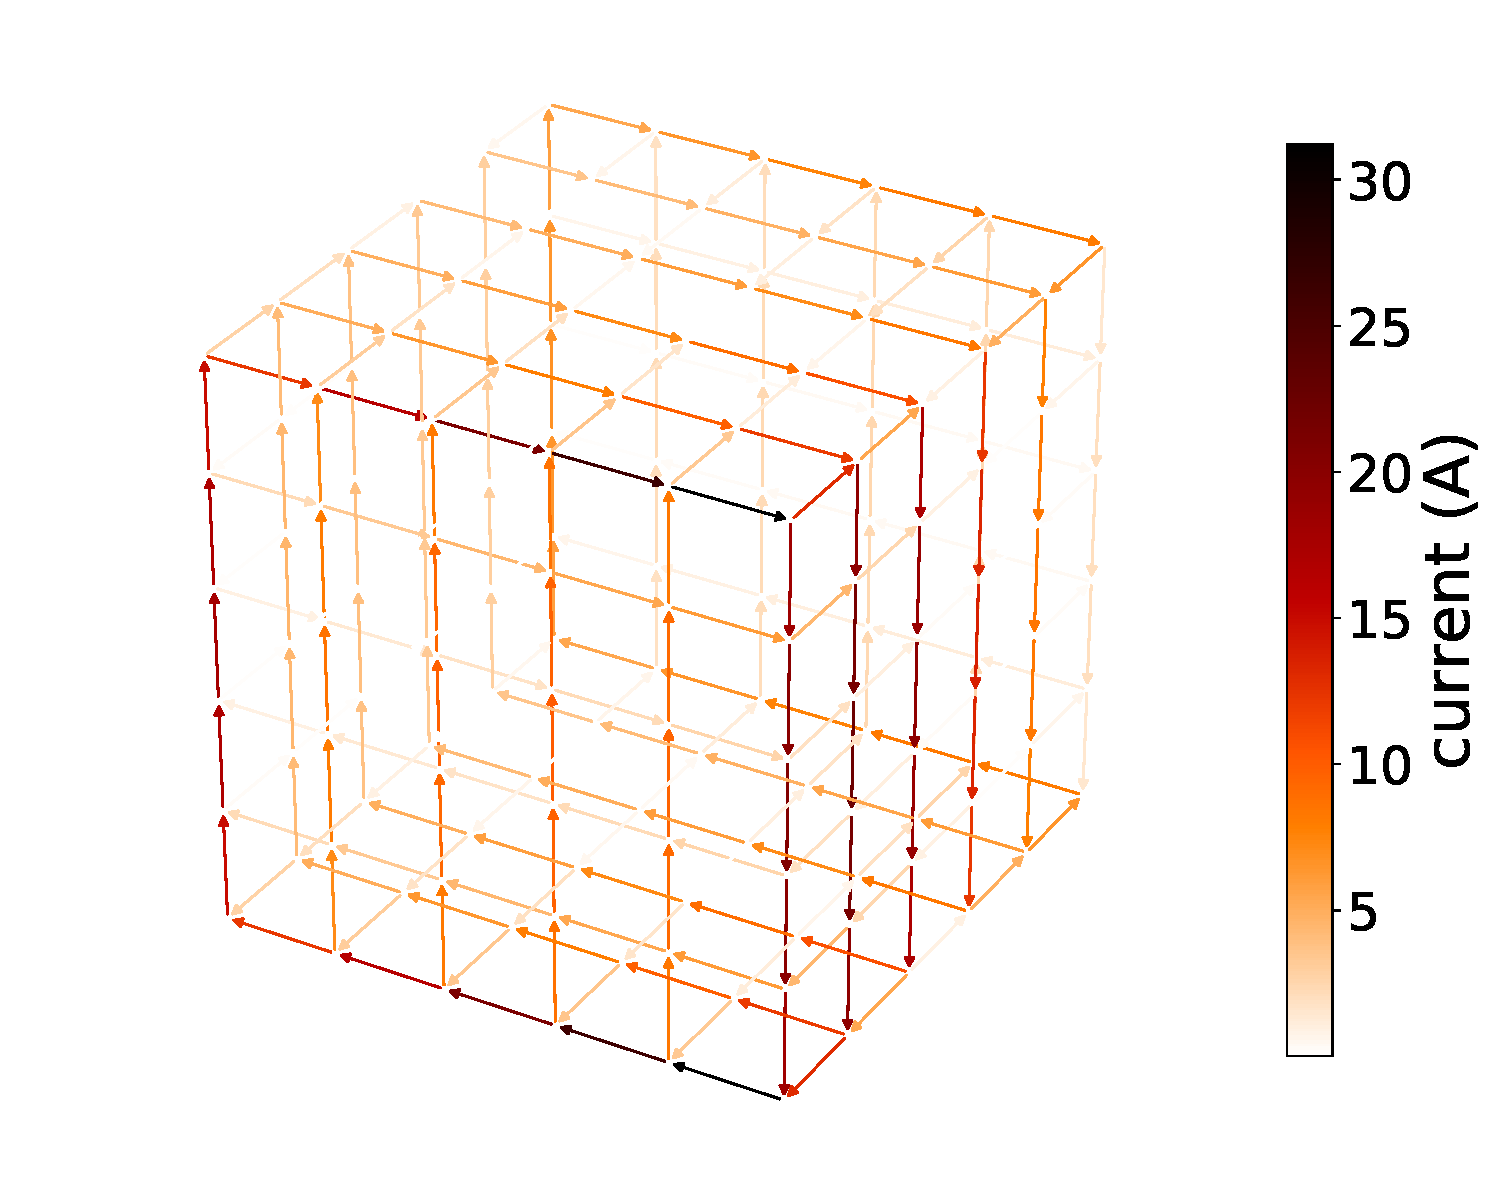
\includegraphics[width=.39\linewidth]{gfx/coils/coil_dipole.pdf}}
  \subfloat{\label{fig:coils_dipole_section}
    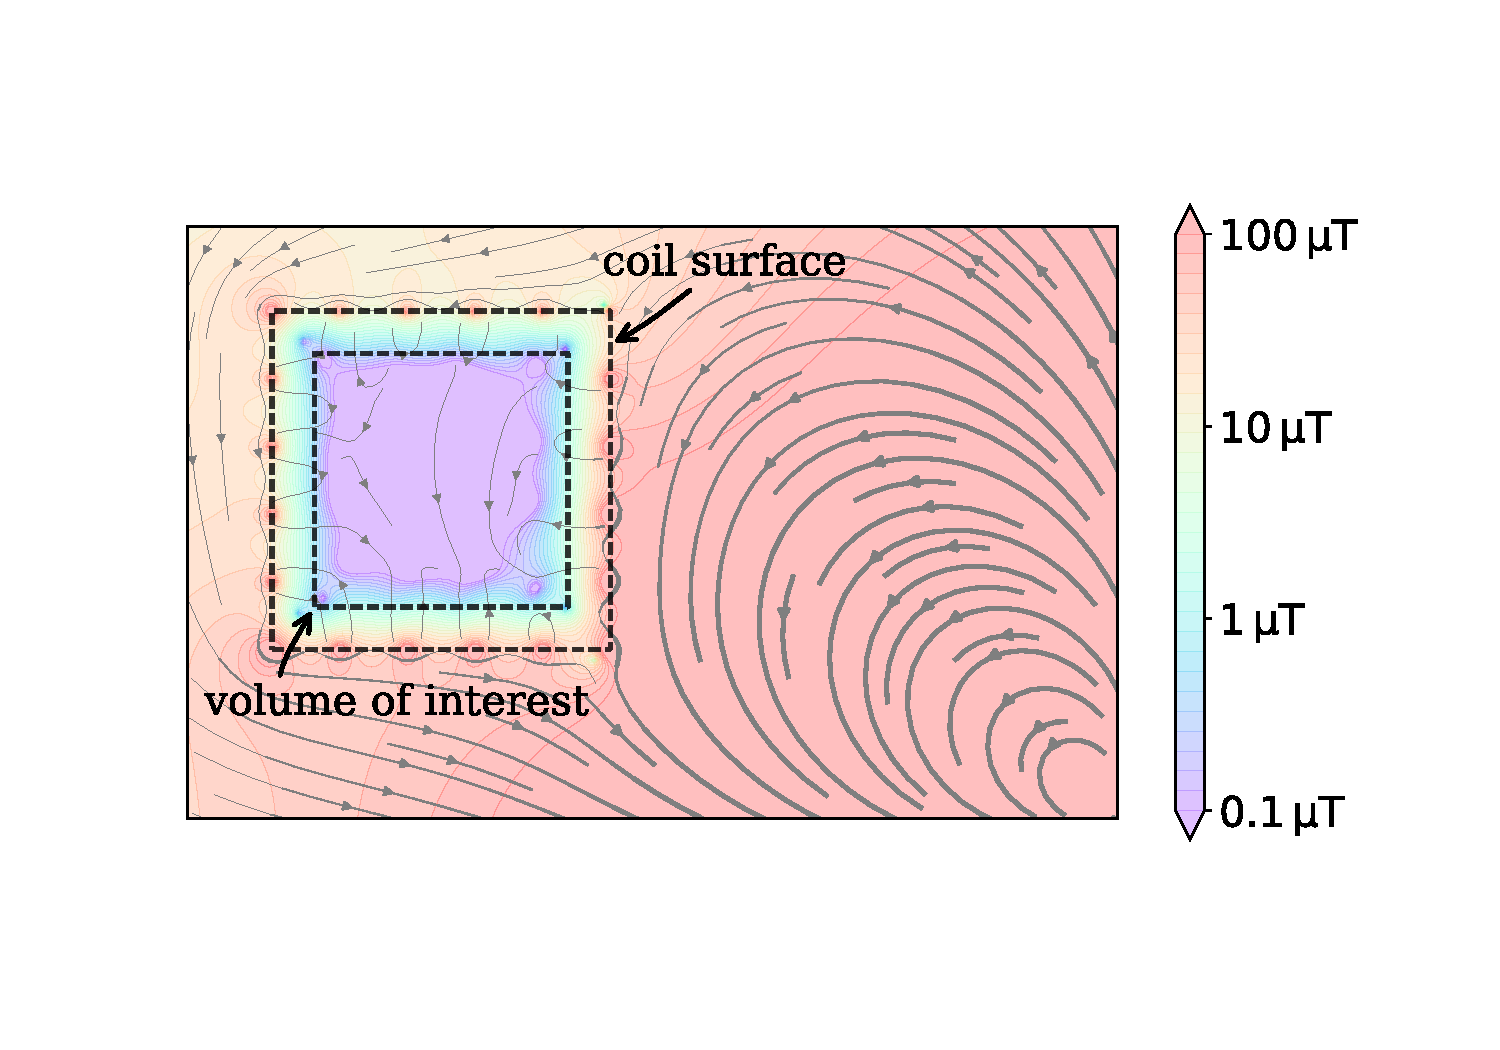
\includegraphics[width=.59\linewidth]{gfx/coils/coil_dipole_section_with_dipole.pdf}}
  \caption{A coil designed on a unit cube with $5 \times 5$ tiles per face to shield against a dipole disturbance. The dipole is located, relative to the center of the unit cube, two units to the right and one unit to the front. It is located in the middle height of the cube. The volume of interest has a side length of \num{0.75}. On the left-hand side the total current along each edge of the dipole compensation coil is depicted. On the right-hand side the magnetic field is shown. The magnetic field lines are shown in grey, the volume of interest and the coil surface with dashed lines. The colors depict the magnitude of the magnetic field (capped at \num{0.1} and \SI{100}{\micro\tesla}). A horizontal cross section in the middle height is shown. The dipole source is located in the lower right corner of the plot and points parallel to the plane of the plot. The magnitude of the field in the volume of interest is reduced from tens of microteslas down to below one.}\label{fig:showcase}
\end{figure*}

Additionally, one can consider constructing dedicated coils to counteract a particular known disturbance. In Fig.\,\ref{fig:showcase}, a showcase design with $N = 6 \times (5 \times 5) = 150$ tiles for compensating a nearby dipole source is presented.

Last, but not least, the method's unique property of designing on a predefined grid makes a large-scale construction particularly feasible. It makes it easy to be incorporated into the existing structures, by defining the grid in a conflict-free way.




\section*{Coil design -- conclusion}
Coil design is a complicated and very technical problem, especially when high accuracy is required. This work presents a method that is simple in terms of both underlying math and computational effort. The design method could find its niche in practical applications, where spatial constraints play a significant role and a percent level in accuracy of the produced field is acceptable. The method has particular advantages when used to design coils of an active magnetic field compensation system. In the next chapter, its application to construction of a compensation system at the ETH Zürich is described.

The software implementation of the coil design, including examples, has been published as open-source~\cite{Coilsjlcode}.

\chapter{Mapping}
A mapping campaign is planned in the experimental hall, where the n2EDM experiment is going to be located. There are numerous magnetic sources in the vicinity of the site, causing the magnetic environment to be unusually complex. Taking a number of magnetic field maps will provide knowledge necessary to make sure, that the n2EDM compensation system will be able to cope with the environment. A 2.5m high mobile tower with 10 3-axis magnetic field sensors has been constructed. The position and orientation of the tower is measured with cable extension transducers, which makes the mapping process as simple as sweeping an area with the tower. Reproducibility of the maps measured with the device was proven to be better than \SI{0.5}{\micro\tesla}.


\section{The idea}
The precision is not crucial, but the time it takes to measure a map is. The shorter it takes to make a map, the less it is influenced by external conditions. It cannot always be mapped during ,,quiet periods''. We want to have maps of magnetic fields that occur only during busy day-times. For example the crane, or SULTAN or other magnets.

For these reasons it has been decided, that the mapping would consist of a tower. The tower would be moved manually (don't use the future tense here), the position and orientation measured along the magnetic field. Then describe the setup here, briefely. The scalar information is enough to localise sources of magnetic field.

Vector information is useful if the data are to be used for example to calculate dedicated compensation coils for some sources of disturbance.

The setup is shown\ldots The mapper was a tower this and that high, with ten fluxgate magnetometers mounted on it.
The three analogue string potentiometers were mounted on a rigid L-piece. The base element is the string potentiometer. It consists of a wire wound on a spring-loaded spool, the spool attached to a potentiometer. For maximal linearity it is constructed in a way, that the string is wound one in layer only. The string string potentiometers give an analogue signal proportional to the extension of the wire. This information was used to determine the position and orientation of the tower.
\marginpar{Other names for a string potentiometers include: cable-extension transducer, draw-wire sensor and string pot.}
\mnote{The terms like the tower need to be clear by here.}


Let us start with a two-dimensional problem. Span two strings between a magnetic field sensor, each to a fixed position in the room. Based on trilateration. With two strings there are two solutions, but we are always able to detect the correct one.

To get the vector information about the field, also the orientation of the sensors needs to be known. For that an arm can attached to the sensor and a third string spanned to the arm's end.

Now is the time for the nice drawing of the geometry solution.



\section{Principle of a string-potentiometer--based mapper}
For a given signal of a calibrated string potentiometer the points where the free end of the string can be make up a circle. The centre at the location of the body of the sensor, the radius equal to the extension of the wire. In the mapper setup there are two string potentiometers mounted on the fixed L-piece, both extended to a single point on the tower. This points lies on the intersection of the two circles. The problem of determining the location based on the measurement of the distances to a set of fixed points is called \emph{trilateration}.

\marginpar{Other position determination methods include triangulation (measurement of angles between lines connecting a set of fixed points) and multilateration (measurement of the differences of distances between a set of fixed points).}

\begin{figure}
  \centering
  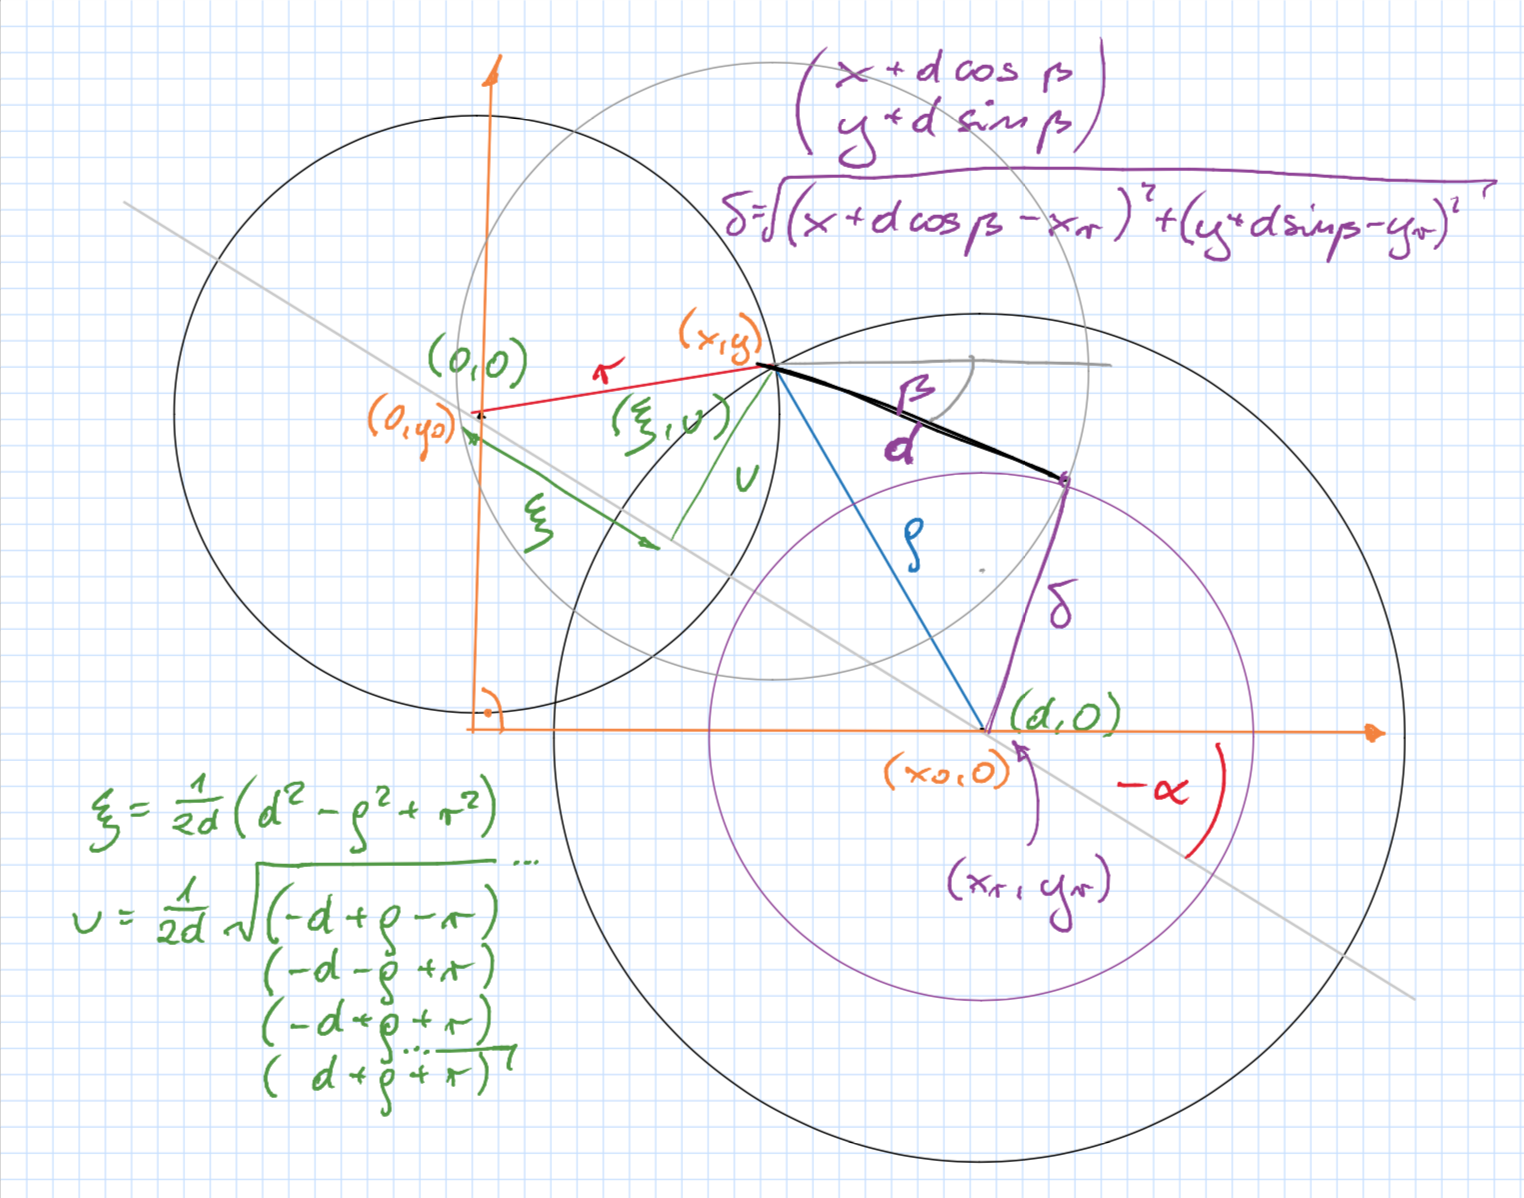
\includegraphics[width=0.9\linewidth]{gfx/mapping/geometry.png}
  \caption{\ldots}
  \label{fig:mapping_geometry}
\end{figure}

The geometry is presented in Fig.\,\ref{fig:mapping_geometry}.The two string potentiometers used to determine the position are located is points $(x, y) = (0, y_0)$ and $(x_0, 0)$ (in the L-piece coordinate system, orange in the figure).
The tower, here point-like, is at $(x,y)$.
The wire extensions are $r$ and $\rho$. For the sake of simplicity, we first give the solution in the coordinate system depicted in green \note{maybe use the A B and C names here already}, where the first string potentiometer is in $(0,0)$ and the second in $(d, 0)$ (with $d = \sqrt{x_0^2 + y_0^2}$). In this coordinate system the tower is in $(\xi, \nu)$. From simple geometry the solution for the position of the tower is:
\begin{align}
  \xi & = \frac{1}{2d} \left( d^2 - \rho^2 + r^2 \right) \\
  \nu & = \frac{1}{2d} \sqrt{ (-d + \rho - r) (-d - \rho + r) (-d + \rho + r) (d + \rho + r) }
\end{align}
The transformation to the L-piece, orange, coordinate system is rotation by the angle $\alpha = \mathrm{ctan} \frac{y_0}{x_0}$ followed by a translation:
\begin{equation}
  \begin{pmatrix}
    x \\
    y
  \end{pmatrix}
  =
  \begin{pmatrix}
    \cos \alpha & -\sin \alpha \\
    \sin \alpha & \cos \alpha
  \end{pmatrix}
  \begin{pmatrix}
    \xi \\
    \nu
  \end{pmatrix}
  +
  \begin{pmatrix}
    0 \\
    y_0
  \end{pmatrix}
\end{equation}

\note{Give here a general formula for an intersection of two circles. Need to check the LabVIEW code?}

With two circles there are two solutions, symmetric around the line connecting the centres of the circles. However, during the mapping the tower stays in the area inside the positive quarter of the L-piece coordinate system.
We assume never to be in the small triangle to the left and down from the line connecting the two string potentiometers.

The problem of determining the orientation of the tower is, in fact, the same as the one of the position. The setup includes a third string potentiometer, with the string attached to \note{there are two $d$s in the picture!} an arm of the tower (depicted in violet in Fig.\,\ref{fig:mapping_geometry}) of the length $a$. The end of the arm lies on the intersection of two circles: the one centred in the centre of the tower and radius $a$, and the one centred at the sensor end of the third potentiometer with the length equal to the wire extension.



\section{LPSC campaign}
First the setting. Magnetic characterisation of a new laboratory room, designated for Hg-199 magnetometry research.
A picture of the room (and the mapper, too?).

The setup is shown\ldots The mapper was a tower this and that high, with ten fluxgate magnetometers mounted on it.
The three analogue string potentiometers were mounted on a rigid L-piece (give the positions).
\marginpar{A string potentiometer has a spring-loaded spool attached to a potentiometer. For maximal linearity it is constructed in a way, that the string is wound one layer only.}
\marginpar{Technical details of the setup: fluxgate -- Stefan-Mayer FLC3-70, readout frequency -- xxx, ADC -- aoethu, string potentiometers -- Micro-Eplison xxx}

Then about the reproducibility.

The subject of this report is a mapping of the magnetic field performed in Laboratoire de Physique Subatomique & Cosmologie (LPSC) in Grenoble, France in the days 6.-10.03.2017 by Michał Rawlik, with the much appreciated help of Rémi Faure, Guillaume Pignol and Dominique Rebreyend.

The goal was to map two rooms, Bastille and Chalet, considered to host a test setup for Hg-199 magnetometry. The setup is sensitive to ambient magnetic fields. In particular, gradients above roughly 10 nT/cm cause an increase in the depolarisation rate of the mercury atoms.

To map the field a device called simply the mapper was used, described below.

This report is bundled with photographs documenting the measurement process, the datafiles taken and plots produced in the analysis. All the analysis code is part of this report. The report is a jupyter notebook using python3 code.


The picture above shows the two main parts of the mapper. The first is the movable tower equipped with 10 3-axis Stefan Mayer FLC3-70 fluxgates. The second is the stationary coordinate sytem onto which three WDS-15000-P115-SA-P string extension transducers (also called string pots) are attached. The string pots are equipped with a custom made attachments that allow the string to come at an angle out of the device. The strings are attached to the tower, two to a point where the vertical beam with fluxgates are, one to one of the arms with wheels. This allows for determination of both position and orientation of the tower.

The data acquisition system is located on a cart. It consists of a power supply used to put a constant current through the string potentiometers, custom-built crate for the fluxgates, which supplies them with power and conditions the incoming signals, and a National Instruments PXI crate, reading the analogue voltage signals from the fluxgates and the stringpots. The digitisation of all signals is simultaneous.

The picture below shows a panoramic view of the room.

The coordinate system is visible in the lower-left corner. To the right are the entrance door, in the middle a power outlet box is visible. Behind the wall with the power outlet box there is a pump, which has been at some point removed. The room is a wooden structure built in a hall. The hall is made of steel beams and sheets. The room's wall with the power outlet is located close, less than 1 metre, to the steel wall of the hall. The hall features a gantry crane, several metres above the roof of the room. On the roof of the room there are air conditioning devices, standing about a metre above the roof on steel legs. The legs have rather large feet, possibly with a steel plate inside.



\section{PSI campaign}

Acknowledge that it is a joint work with Solange Emmenegger.

Describe the changes to the setup: now the geometry is like this and this. Need probably a detailed picture of the geometry of the setup and the mapper.

About the method to fit the calibration parameters to the fixed points.

% -------------------------------------------------------
% AXION SEARCH
% -------------------------------------------------------
\part{Axion--Like particles search}
% !TEX root = ../rawlik-phd-thesis.tex
\chapter{Axion analysis}
\label{ch:axion-analysis}

Now that the foundation of the analysis has been introduced, we describe how it was applied to look for oscillations in the neutron EDM data taken at the PSI in the years 2015--17.

First we considered the scalar coupling, acting like an oscillating nEDM signal. We analysed directly the time series of $R$, measured with every cycle of the experiment. This allowed us to consider frequencies up to inverse \SI{300}{\second}, but, on the other hand, required a careful consideration of the effect that on oscillating nEDM would would have on the $R$ time series. Not having found a signal, we could interpret this analysis as the first laboratory limits on the axion coupling to gluons.

The work described in this chapter was a joint effort with Nicholas Ayres, who analysed the data of the Grenoble-based nEDM measurement~\cite{AyresThesis} in search for the scalar coupling. Rather than the raw $R$ time series, he considered the one of the nEDM estimates as obtained on a run basis. The two analyses were complimentary, each covering a different range of oscillation frequencies.

Then we discuss a different coupling, a vector one, acting like on oscillating magnetic field. No significant discovery could be claimed here, which led to exclusions for the axion-nucleon coupling.

Finally, we considered a particular frequency of \num{23.934}~hours, the sidereal frequency.
\marginpar{The sidereal frequency is the one of the Earth spinning in the celestial coordinates.}
Oscillations of that periodicity can be interpreted a hint of a \emph{cosmic spin anisotropy field}~\cite{Altarev2009}.



\section{How a signal would look like}
We start by considering, how an oscillating electric dipole moment would have come up in the $R$ time series, as measured by the PSI experiment.

The main purpose of the experiment was to measure the static neutron electric dipole moment. This would appear as a shift in $R$ dependent on direction of the electric field relative to the magnetic one. In a zero electric field there would be no shift, while the parallel and anti-parallel configurations of the magnetic and electric fields would shift $R$ in opposite directions. Due to the data blinding
% \footnote{In order to reduce bias the data were modified upon being taken in a way, that a secret nEDM was injected into them. This additional offset is only revealed as the very last step, once the measurement and analysis have been completed. The data were still blinded at the time of writing.}
we expect a pronounce shift corresponding to an nEDM of \SI{e-25}{\elementarycharge\centi\meter}.

Should the neutron electric dipole moment oscillate, $R$ would oscillate as well, even if the electric field is kept constant. A reversal of the electric field polarity would reverse the phase of the oscillations. At zero electric field no oscillations would be visible. In the PSI experiment the field was automatically changed according to the looped pattern: 48 cycles in one polarity, 8 cycles without the field, 48 cycles in the other, 8 without the field. In Fig.\,\ref{fig:axions_data_taking_one_run} we depict an $R$ time series with the combined effect of a large nEDM oscillation and the blinding offset.

\begin{figure}
  \centering
  \subfloat[An oscillating neutron electric dipole moment signal in the nEDM @ PSI apparatus. The colours indicate different electric field states: parallel to the magnetic field, antiparallel to it and zero]
  {\label{fig:axions_data_taking_one_run}
  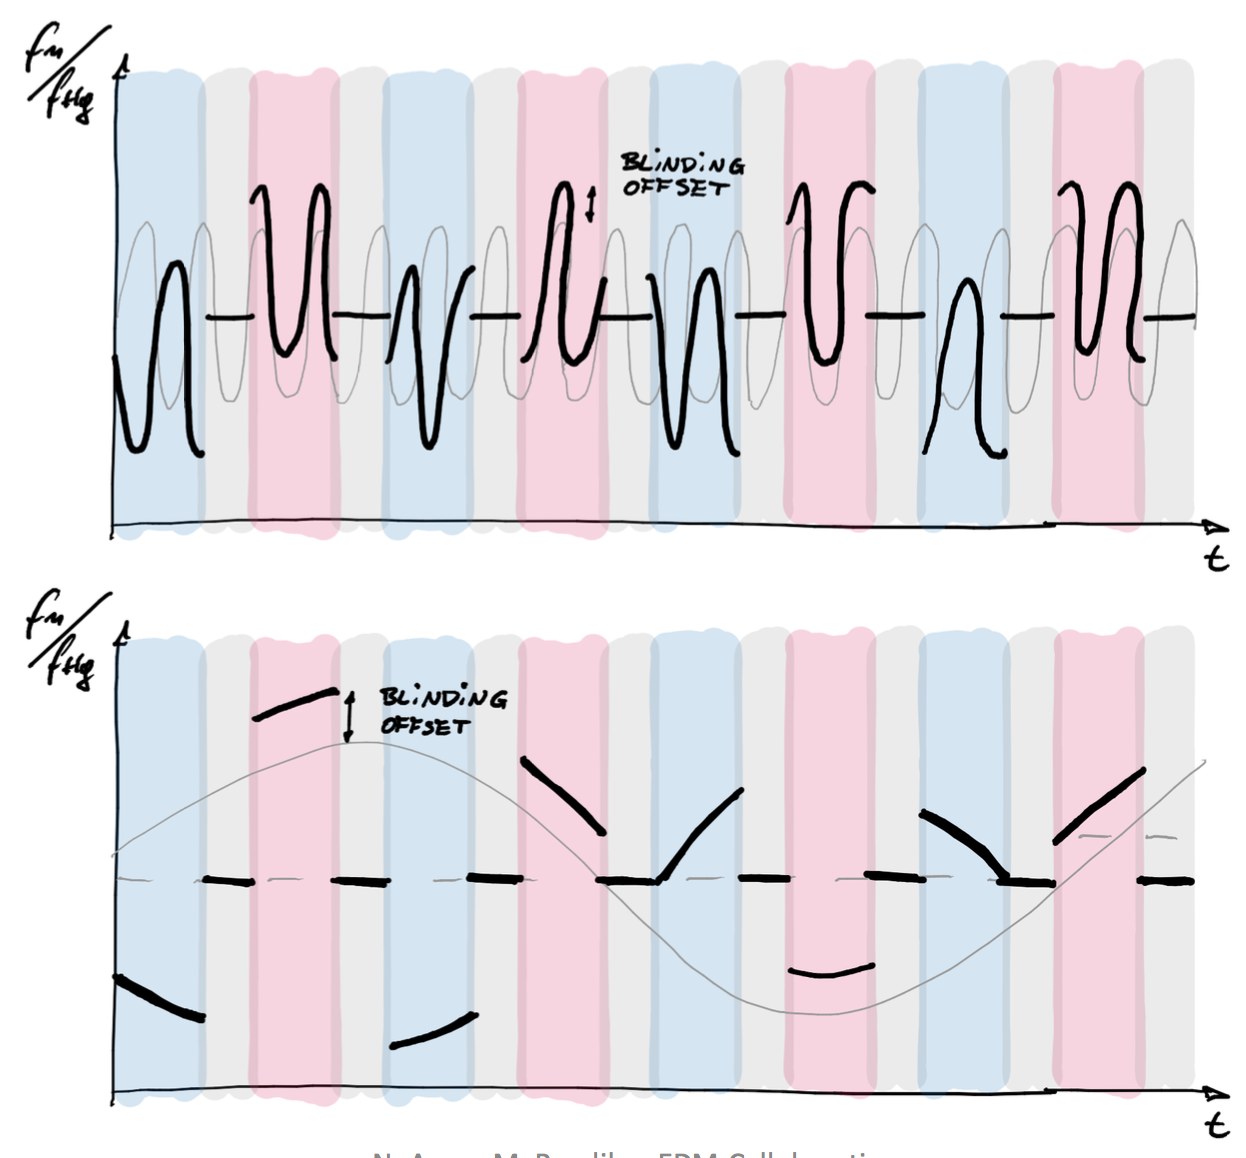
\includegraphics[width=.34\linewidth]{gfx/axions/cycle-level_blinding_offset.png}}
  \quad
  \subfloat[An oscillating neutron electric dipole moment signal in the nEDM @ PSI apparatus across many runs. The colours indicate different electric field states: parallel to the magnetic field, antiparallel to it and zero. Different runs have different magnetic field gradients, which causes each run to have a different shift in $R = f_n / f_{Hg}$.]
  {\label{fig:axions_data_taking_runs}
  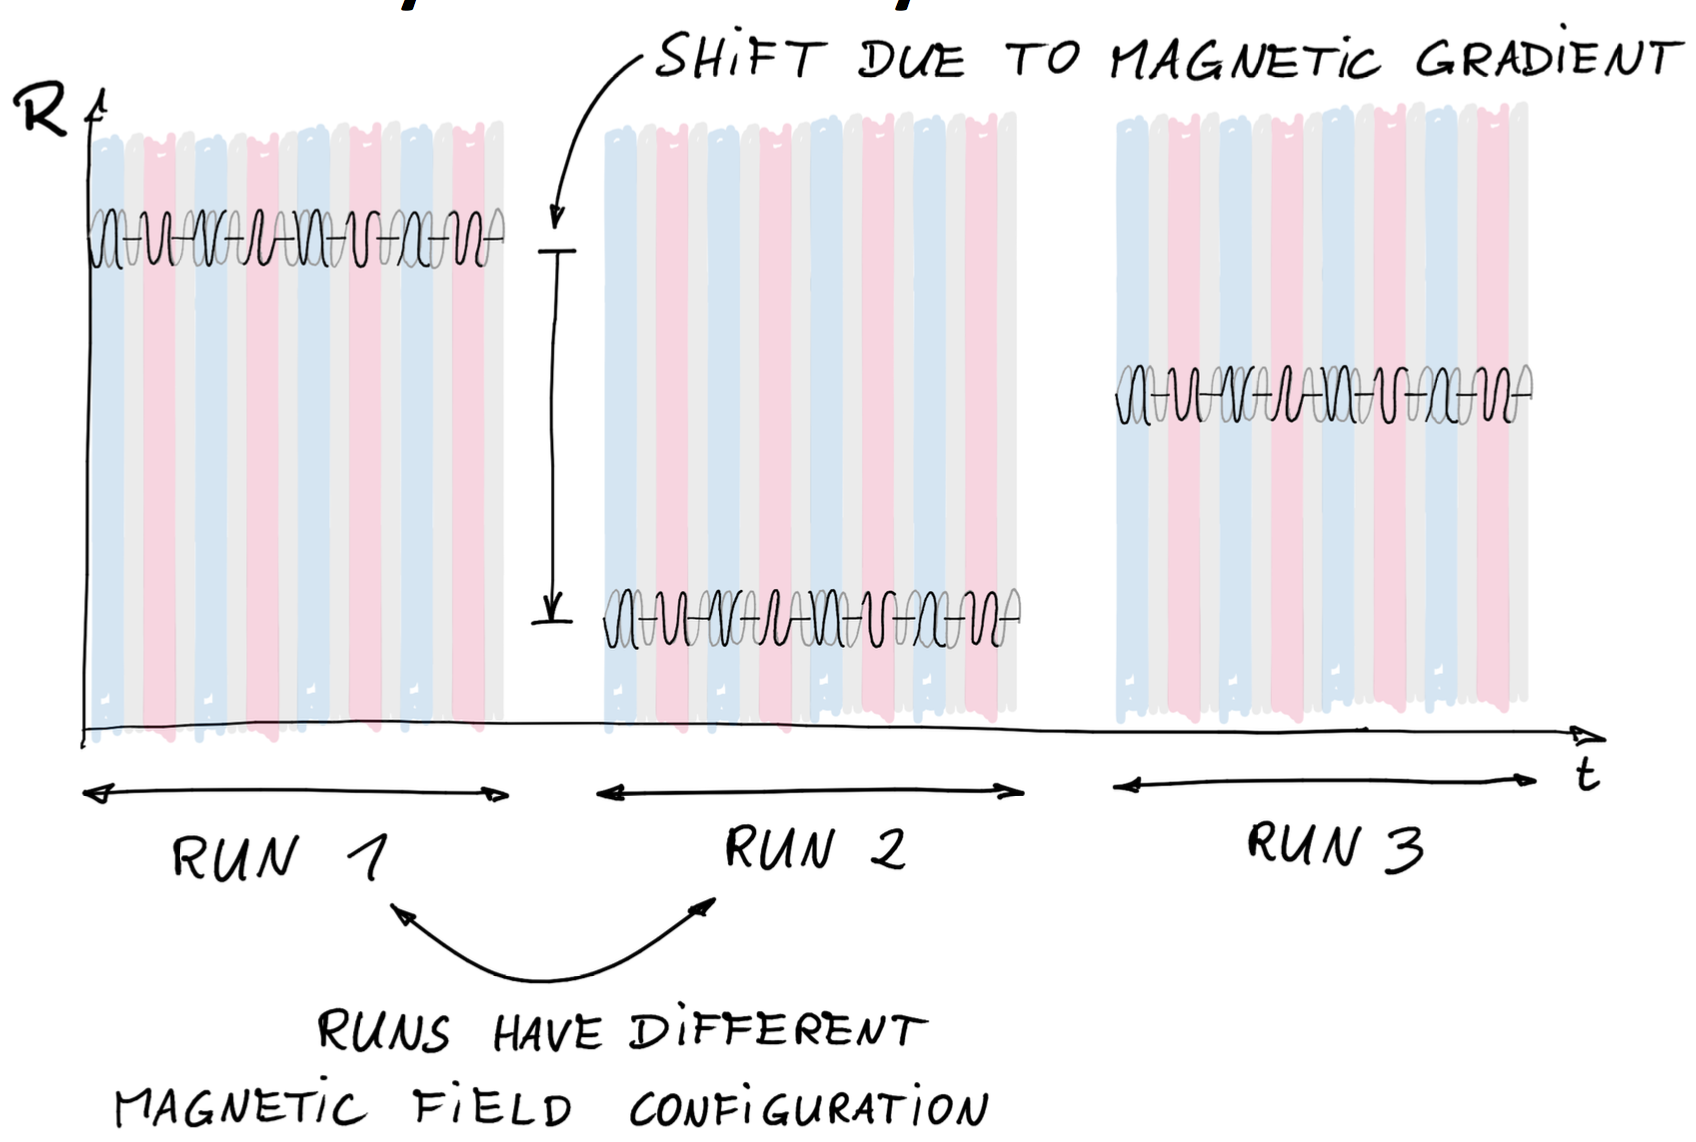
\includegraphics[width=.56\linewidth]{gfx/axions/cycle-level_gradient_jump.png}}
  \caption{The data taking scheme in the nEDM experiment at PSI.}
\end{figure}

Of course, the least-squares spectral analysis could not be applied directly to the complicated $R$ time series. Note, that the time series is still a part of a harmonic oscillation, when only one electric field polarity is considered. Or, to be exact, one relative configuration of the electric and magnetic fields. In the analysis the $R$ time series was split according to this condition into three: one without the electric field (not sensitive to an oscillation of nEDM), one with the electric and magnetic fields parallel and one with anti-parallel. The last having the hypothetical oscillation in the opposite phase then the parallel one. We will refer to the three data sets as $E=0$, $E \uparrow \uparrow B$ and $E \uparrow \downarrow B$, respectively. Each of those was treated separately.

% \begin{figure}[bth]
%   %FIXME directly copied from Elise's presentation on the 2015 PSI collaboration meeting
%   \myfloatalign
%   \subfloat
%   [Another time series of $R$ in the nEDM experiment. The colours depict electric field states, black being no electric field. A drift is clearly visible.]
%   {\label{fig:axions_gradient_drift_not_corrected}
%   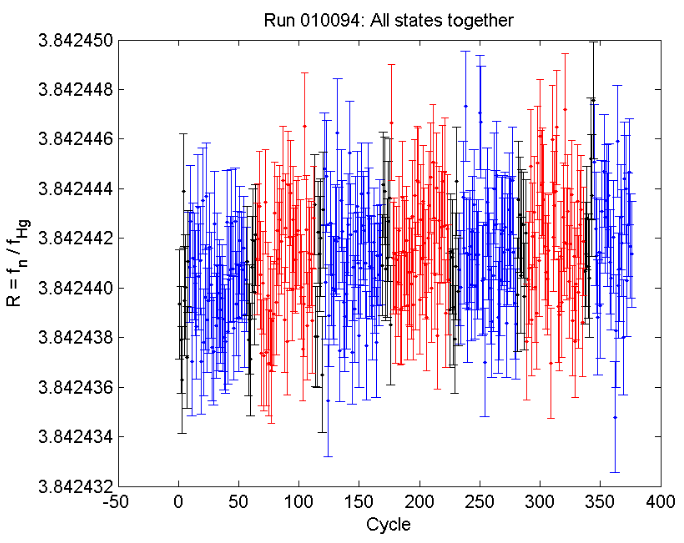
\includegraphics[width=.45\linewidth]{gfx/axions/gradient_drift_elise}}
%   \quad
%   \subfloat
%   [The data as on Fig.\,\ref{fig:axions_gradient_drift_not_corrected} corrected for gradient fluctuations.]
%   {\label{fig:axions_gradient_drift_corrected}
%   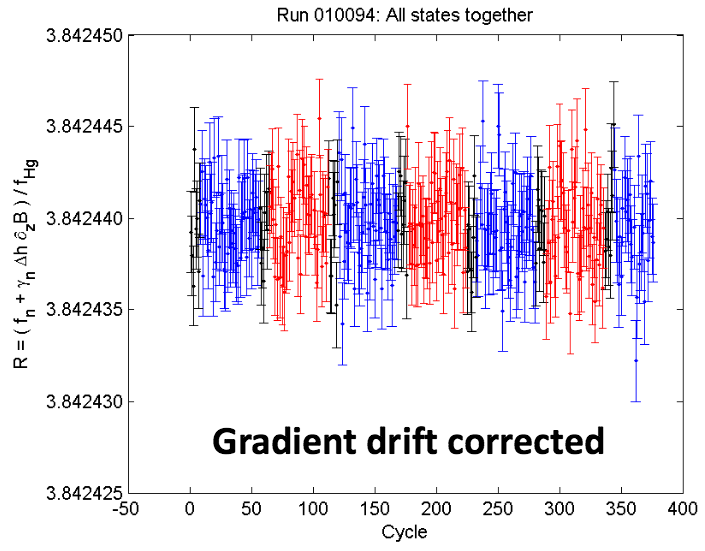
\includegraphics[width=.45\linewidth]{gfx/axions/gradient_drift_elise_corrected}}
%   \caption{Correcting the $R$ time series for fluctuations of the vertical magnetic field gradient.}
%   \label{fig:axions_gradient_drift_correction}
% \end{figure}

There are other effects in the $R$ time series. A part of the measurement procedure was to deliberately work in a magnetic field gradient, as discussed in Sec.\,\ref{sec:measurement_procedure}. The vertical magnetic field gradient changed substantially between sequences. Thereby $R$ was affected by a big value, changing the DC level of the oscillating nEDM signal, as illustrated in Fig.\,\ref{fig:axions_data_taking_runs}.

The problem of inter-sequence jumps was solved by allowing the DC offset in the LSSA fit to be different in each sequence:
\begin{equation}
  \label{eq:axions_LSSA}
  A\sin(2 \pi f t) + B\cos(2 \pi f t) + \sum_i C_i\,\Pi_i(t) \ ,
\end{equation}
where $C_i$ is the free offset in the $i$th sequence and $\Pi_i(t)$ is a gate function equal to one in the $i$th sequence and zero elsewhere. In this way the model explicitly assumed coherence of the oscillation across sequences. However, the downside was a reduced sensitivity to oscillations slower than a sequence (2--3 days), as they could be absorbed into the different free offsets. This, together with the split into three series, reduced the problem to one described in the previous chapter.

% It may be tempting to think about demodulating the $R$ time-series into what would be expected to be an oscillation. This would require subtracting the DC offset for each electric field configuration, in each run separately, then flipping the signal around the DC level for one configuration. \mnote{The offsets are measured with Cs, mention that.} The disadvantage is that uncertainty in such a demodulation would become a systematic effect and would need to be tightly controlled.

% , as clearly visible in Fig.\,\ref{fig:axions_gradient_drift_correction}.
% The nEDM team spares no effort to measure the gradient. Nevertheless, the achieved precision (\SI[per-mode=symbol]{\approx 1}{\pico\tesla\per\centi\meter}) is only comparable to the one of $f_n$ (in the order of \SI{1}{\pico\tesla}). The exact way how the gradient should determined is highly non--trivial and there is ongoing research in this respect. \mnote{Mention here the exact way the gradient drift correction is done. And cite Elise's thesis.} Actually, even the height difference between the neturons and $^{199}$Hg centres of mass (a few milimeters) is still discussed. \mnote{Know how exactly was $\Delta h$ determined in the end. Also, mention the definition of a sequence here (as in the paper).}
% \cite{Afach2014magmoment}

% Assuming a constant gradient during a \emph{run} one can determine it much more precise. This assumption, however, is known not to be exactly true.

% One should note, that any, including an oscillating one, nEDM effect affects only the position of the neutrons' resonance. The shape of the resonance curve is unaffected. Therefore, the method to extract neutron Larmor frequency $f_n$, and thereby $R$, for each \emph{cycle} is valid also in case of an oscillating nEDM.



\section{Systematic Effects}
In the analysis the compatibility of the periodogram of the $R$ time series with the one of pure noise, the null hypothesis, was tested. Variations in $R$, harmonic in particular, but not only, would have resulted in an additional power in the periodogram and could, therefore, be considered a systematic effect.

Most prominently, $R$ followed the changes in the vertical gradient of the magnetic field. Because of the centre of height difference between the neutron and mercury atom ensembles they saw, on average, a different field in a presence of the vertical gradient.  Luckily, it could be corrected for with the use of the cesium magnetometers. On a cycle basis, a second-order parametrisation of the field was fitted to their readouts, giving an estimate of the gradient~\cite{Afach2014magmoment,WurstenThesis}. Due to unknown random offsets in the magnetometers' readings the correction was only relative---correcting for the variations of the gradient. In between runs the caesium magnetometers were calibrated, which altered the offsets. For this reason the correction could not extend across a run boundary. 
% , which changed in between runs which changing after this correction could only be relative in a run.
% \marginpar{STILL CHANGE RUN TO SEQUENCE!!!}

There could have been, potentially, other effects causing the time series of $R$ not to be fully random. An important decision had to be taken on how to treat those. Two possibilities were considered.

A detail study of time-dependent systematic effect could be performed.
Here any excess in power, in any dataset ($E \uparrow \uparrow B$, $E \uparrow \downarrow B$ and $E=0$) would be treated as a signature of some kind of a signal. All effects that could potentially result in that would have to be identified before the analysis was performed and corrected for. This would have required a long and careful systematic study. Moreover, the full-fledged systematic studies for the constant nEDM analysis of the PSI data were still ongoing at the time. This approach was considered to be, albeit careful, not necessary for this analysis.

% \paragraph{Determine delicate frequencies and cut them out.}
% The experiment run 
% Looking at periodograms of raw data one sees that there are several typical frequencies where peaks appear. Typically at inverse specific time constants at which the experiment operates: cycle separation, day, week, , HV-reversal, B0-reversal. We may decide that all systematic effects are constrained to these frequencies and do not perform the analysis there at all.

% \paragraph{Assume there are no systematic effects.}
Instead, an easier approach was taken. An axion would produce a very specific signal, in particular:
\begin{enumerate}
  \item There would be no signal in the $E=0$ dataset.
  \item The signal would appear in both $E \uparrow \uparrow B$ and $E \uparrow \downarrow B$ datasets, with equal amplitude.
  \item The signals in $E \uparrow \uparrow B$ and $E \uparrow \downarrow B$ data sets would be shifted in phase by \ang{180}.
  \item The signals would have to have a high coherence of $\delta f / f = 10^{-6}$.
\end{enumerate}
In a case when an excess in the power would be observed, it would only be called a candidate for an axion signal, if the three above conditions would have been met. Otherwise, it would be attributed to a, potentially unknown, systematic effect.

Naturally, this made the systematic study dependent of the fact of having found a signal, opening a line of attack on the analysis. The analysis might be claimed not to have the right to exclude signals, because there might have been a systematic effect that cancelled a real signal out, but was never found nor even looked for. Nevertheless, such an event was highly improbable due to the high coherence of the axion field. In order to cancel the axion signal, a systematic effect would have not only needed to be as coherent as the axion field, but additionally fine-tuned over at least 5 orders of magnitude magnitude of tested frequencies. With the coherence of $\delta f / f = \num{e-6}$ this is a tuning of \num{e-30}. It would also have needed to be fine-tuned in amplitude over $\sim 20$ orders of magnitude, which gives a rough estimate of the cancellation probability of \num{e-50}. As the exclusions are anyway probabilistic in nature, in this case a 95\% C.L. threshold is claimed, we consider this approach to be justified.




\section{The PSI 2015--16 data set}
\note{uniform spelling of data set}

% What is it that I really want to communicate here? First introduce the time series and point to the plot. Then explain the structure by walking the reader through the plot!

\begin{figure}
  \centering
  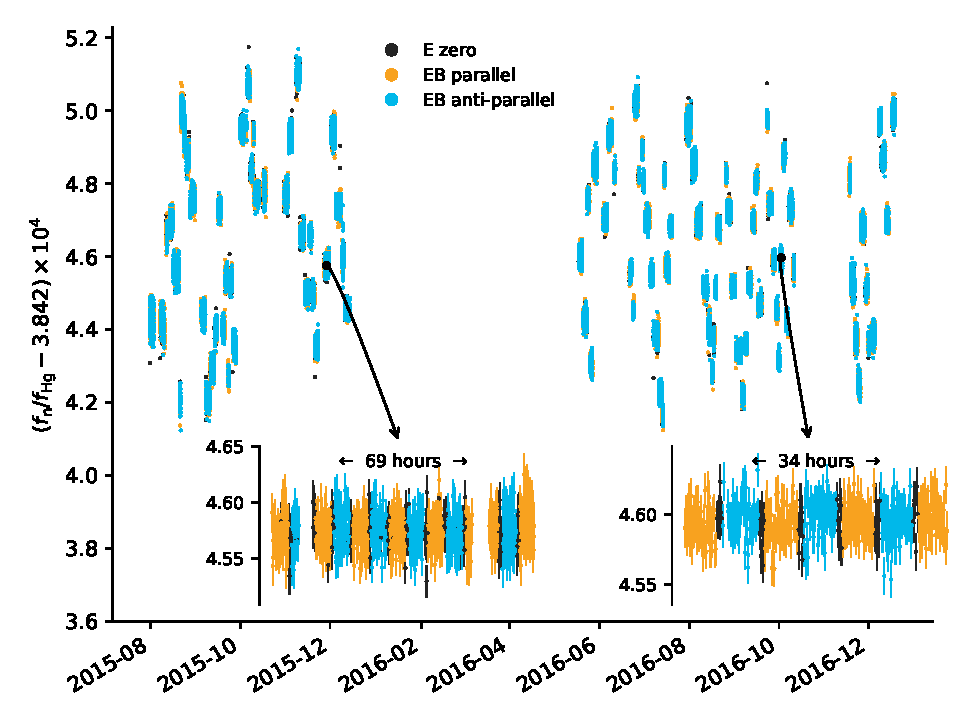
\includegraphics[width=0.9\linewidth]{gfx/axions/deltah4mm_time_domain_inset_no_yerr.pdf}
  \caption{The complete PSI data set used in the analysis. It spans from July 2015 to December 2016. Two sequences are enlarged. Due to high density of the measurements individual points cannot be resolved. Each point is plotted with its error bar. The colours depict the relative orientation of the magnetic and electric fields: $E \uparrow \uparrow B$ (orange), $E \uparrow \downarrow B$ (blue) and $E=0$ (black). The $R$ time series has been corrected for gradient drifts.}
  \label{fig:PSI_dataset_time_domain}
\end{figure}

The data used in the analysis were collected in PSI between 2015--07--03, 14:21:30 and 2016--12--18, 19:51:23. The measurements were performed primarily to obtain the estimate of the constant nEDM\@. The time series of the ratio of the precession frequencies of the neutrons and mercury atoms $R = \nu_\text{n} / \nu_\text{Hg}$ is presented in Fig.\,\ref{fig:PSI_dataset_time_domain}.

\marginpar{A technical term for uninterupted operation was a run. Sometimes a run was stopped due to technical reasons a new started afterwards. A sequence combines those consecutive runs, that could be one run if not for the interruption.}
Take a look first at the inset in the lower-right corner. It zooms into data collected within one \emph{sequence}, typically 1--3 days long.
During a sequence the apparatus completed one cycle after another, one every \SI{300}{\second}, each yielding an estimate of $R$.
The electric field was automatically changed between three states: pointing upwards, being zero and pointing downwards. The different relative orientations of the electric and magnetic fields are depicted in colour in the figure. Sometimes there were technical breaks in the data taking during a sequence, as in the case of the one shown in the lower-left corner of Fig.\,\ref{fig:PSI_dataset_time_domain}.

% Here what it is and what's done Sometimes the automatic process was interrupted, but the sequence still continued, as seen in the other inset.

% REFER TO WHAT WAS IN HOW THE SIGNAL WOULD LOOK LIKE! But, repeating a bit will not hurt. The reader should already be prepared, now just reiterate.

% \mnote{Idea: present a scheme of the timing structure of the nEDM data taking, where a cycle, sequence are defined, and HV and B field reversals are shown.}
% The time structure ias follows: The atomic measurement is called a cycle, which gives an estimate of the average precession frequency of the neutrons $f_\mathrm{n}$ and mercury $f_\mathrm{Hg}$. Their ratio $R = f_\mathrm{n} / f_\mathrm{Hg}$ is show in Fig.\,\ref{fig:PSI_dataset_time_domain}. An automatic system executes one cycle after another (triggered on a signal from the UCN source). A series of automatically executed cycles is called a \emph{run}. The $R$ time series of a typical run, 1-3 days long, is shown in the lower-right corner. During a run the electric field automatically changes polarity every \ldots \mnote{Find out how many cycles for one HV cycle} cycles. In between \ldots cycles with no electric field are measured. These have no sensitivity to the electric dipole moment, but provide a control data set.

A sequence was taken always in one magnetic field configuration. The in-sequence variations of the vertical gradient of the magnetic field $\partial_z B_z$ were corrected for using the field model fits to the readings of the Caesium magnetometers. In between the sequences the vertical gradient was changed in \SI{10}{\pico\tesla} steps, up to \SI{60}{\pico\tesla}, so that those systematic effects, which scale linearly with the gradient, could be extrapolated to zero (see Sec.\,\ref{sec:measurement_procedure}). These large changes in the vertical gradient caused the large shifts in $R$ from sequence to sequence.

The $R$ time series was sliced into three separate based on the relative direction of the magnetic and electric fields: $E \uparrow \uparrow B$, $E \uparrow \downarrow B$ and $E=0$. In each a search for a harmonic oscillation was performed.

% During a single run the magnetic field is kept as stable as the team can manage. The drifts of the homogeneous part of the field are cancelled in $R$, but the gradients are not. So drifts of the gradient directly cause changes in $R$. These, however, can be corrected for using the Cs magnetometers. They are mounted on the top and bottom electrode and they can be used to correct for the in-run gradient drifts. They do not provide an accurate measure of the gradient. \mnote{Remember the reasoning why the cross-run gradient-drift correction can't be done: to large a change and the calibration issues}.

% Sometimes for technical reasons there is a pause in the measurements. Then the collected data may still belong to one run One such sequence is shown in the lower-right inset in Fig.\,\ref{fig:PSI_dataset_time_domain}.

% Typically... Sometimes stopped... Define a sequence



% Really, really first, show some example runs. 



\section{The analysis itself}
\begin{figure}
  \centering
  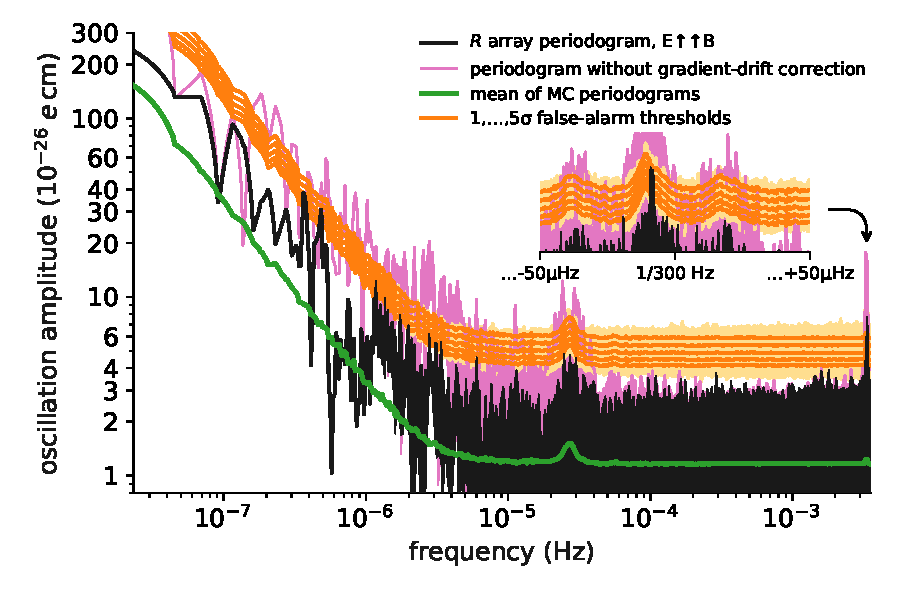
\includegraphics[width=0.9\linewidth]{gfx/axions/detection_psi_inset_gc.pdf}
  \caption{Periodogram of the $R$ time array of the PSI experiment data, sensitive to oscillations in the quantity $d_\mathrm{n} - \left( \mu_\mathrm{n} / \mu_\mathrm{Hg} \right) \, d_\mathrm{Hg}$, taken with the $\boldsymbol{E}$ and $\boldsymbol{B}$ fields parallel (black line).
  The mean of MC--generated periodograms, assuming no signal, is depicted in green. MC is used to calculate $1,2,…,5\,\sigma$ false--alarm thresholds, depicted in light orange.
  For clarity, we also plot the smoothed version in orange.
  There are two regions where a rise in the amplitude is expected, namely around \SI{28}{\micro\hertz} (inverse of 10 hours) and \SI{3.3}{\milli\hertz} (inverse of 300 seconds), due to the time structure of the data taking (see the main text for more details). The periodogram of non-gradient-drift-corrected data is shown in pink.}
  \label{fig:axions_PSI_detection}
\end{figure}

The periodogram of the subset of data with the electric and magnetic field parallel $E \uparrow \uparrow B$ is presented in Fig.\,\ref{fig:axions_PSI_detection} in black. The average null-hypothesis periodogram is depicted in green and the false-alarm thresholds in orange. An inset details the region around inverse \SI{300}{\second}, the cycle frequency.

There are two regions of expected rise in the oscillation amplitude due to the time structure of the data collection.
\marginpar{Recall the discussion in Sec.\,\ref{sec:a_null_hypothesis_test} about the peaks in the periodogram solely due to the time structure of the series.}
The one around \SI{28}{\micro\hertz} (the inverse of 10 hours) corresponds to the period of the reversal of the electric field.
The other, around \SI{3.3}{\mili\hertz}, the inverse of \SI{300}{\second}, corresponds to the cycle repetition rate.
There are five
%\note{NA does anybody know what style guide says about when numbers should be written in words i.e. seven vs 7? I personally think small numbers without units should be words but this comes down to preference} ***I THINK LESS THAN TEN IT IS IN WORDS - MALCOLM ***
trial frequencies for which the $3\upsigma$ false-alarm threshold is exceeded,
%\note{PMM: use words like 'surpassed', or 'exceeded' instead of penetrated}
two of which, including the largest excess with a $6\upsigma$ significance, occur in a \SI{100}{\micro\hertz} region around the inverse of \SI{300}{\second}, while the other three are in the low-frequency region, longer than an inverse length of a sequence.
% \note{FP: Can you maybe also explicitly state the positions of these three lines in Hz or inverse time?}
 The periodograms for the other two datasets, very similar to this one, can be found in App.\,\ref{ch:alp_appendix}.
In the other sensitive set, there are three excesses of the $3\upsigma$ threshold (the highest is $5\upsigma$), all constrained to the same two regions. In the control dataset, only the $1\upsigma$ threshold is exceeded.
%\note{MR: We may consider not discussing the false--alarm threshold penetrations, and just state in the next paragraph that we do not find a signal which meets our criteria.}
The periodogram of the $R$ time array without the gradient-drift correction is shown in pink in Fig.\,\ref{fig:axions_PSI_detection}. The correction has an effect only for frequencies slower than the period of the reversal of the electric field. It is not a 
It is not by chance. The period of the high voltage was chosen to be when the field is stable.  that  to visualize the frequencies where the correction has an effect.

\mnote{Here a brief discussion about the Cs-gradient-drift correction.}
It is interesting to observe, that the periodograms with and without the gradient drift correction diverge only for frequencies below \SI{6e-5}{\hertz}, the period of the high-voltage reversal (the disagreement around inverse \SI{300}{\second} is folded from the low frequencies). This is not a coincidence. The period of the high-voltage reversal has been deliberately chosen, so that\ldots\mnote{Was the period really chosen such?}

No signals fulfilling the detection criteria are found.

Having observed no significant signal, we could place limits on the coupling strength as the function of axion mass.
The result are presented in Fig.\,\ref{fig:axions_limits_coupling} and are labeled \emph{short time-base} (the next paragraph is devoted to the \emph{long time-base} limits).
The limits we evaluated using Monte Carlo techniques, as described \ldots.
The results are presented in the landscape of already existing limits: axions with a mass below \ldots have their Compton wavelength larger than the size of the smallest dwarf \emph{galaxies} and, therefore, could not be the sole constituent of dark matter; the influence of axions in the red-shaded area on the \emph{Big Bang nucleosynthesis} would result in an underproduction of\ldots
\mnote{Need to research and explain all those.}

\begin{figure}
  \centering
  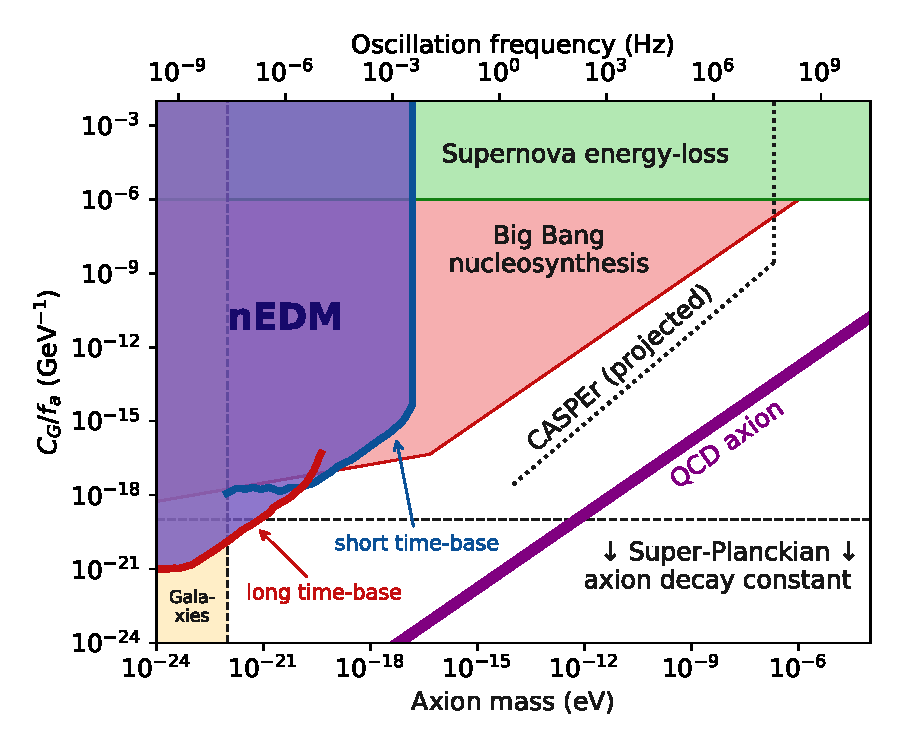
\includegraphics[width=0.9\linewidth]{gfx/axions/psi_ill_axion_limits_v7.pdf}
  \caption{Mention, that it shows\ldots}
  \label{fig:axions_limits_coupling}
\end{figure}

The Fig.\,\ref{fig:axions_limits_coupling} features the \emph{short time-base} limits, the ones described in this work, as well as \emph{long time-base} ones.
This work was performed with close collaboration with Nicholas Ayres of the University of Sussex. The Sussex group was part of the collaboration running the predecesor of the nEDM experiment at PSI --- the measurement performed in the Institute Laue-Langevin in Grenoble, France, in the years 1998--2002~\cite{Pendlebury2015}.
An analysis analogous to this work was performed on those data, with an important difference, which made it sensitive to lower frequencies (or lighter axions)~\cite{AyresThesis}.
Namely, the time series consisted of one point per run, in contrast to one per cycle in the short time-base analysis.
On one hand it limits the sensitivity to oscillation periods corresponding to one run (1--2 days).
On the other, the sensitivity to low frequencies is not deteriorated, as there is no need to use multiple free offsets in the LSSA fit (Eq.\,(\ref{eq:axions_LSSA})). In fact the free offset is assumed to be zero on the ground that the experiment delivered a zero-compatible result.
% in the process of calculating the per-run nEDM estimate the gradient fluctuations are averaged out, so there is 
\mnote{What about the gradient-related systematics (nEDM vs R' curve)? Was it corrected for? Wrote an email to Nick.}

Despite close collaboration the two analyses shared no common code. As a mean of cross-check, the two codes were compared on artifical datasets, more on that in the appendix.




\section{False-alarm thresholds}
\mnote{In this section we will dive in more deeply into statistics associated with the data.}

Remind: for each of the three data sets we have a periodogram, one value for the power estimate for each frequency. Then we have a collection of simulated periodograms, many power estimates for each frequency, generated assuming the null hypothesis --- only white noise in the data.

First how the local p-values were obtained. In Fig.\,\ref{fig:P_best_signal_candidate} the cumulative distribution function (CDF) \mnote{define CDF somewhere and then just continue to use it. Maybe even a table of abbreviations at the end?} of the power at one frequency (a special one, where the least probable peak is). CDF has this advantage over the PDF, that it does not require binning to be estimated. To estimate the CDF all the MC-generated power estimates are sorted into an array. Then the discrete CDF estimate is plotted by putting the power on the x-axis and the place in the sorted array, normalised to one, on the y-axis. Fig.\,\ref{fig:P_best_signal_candidate} actually shows $1 - \mathrm{CDF}$, so that the logarithmic y-scale can be leveraged to resolve the high-power tail. The plot also includes a extrapolating fit line and false--alarm thresholds, which we now proceed to explain.

\begin{figure}
  \centering
  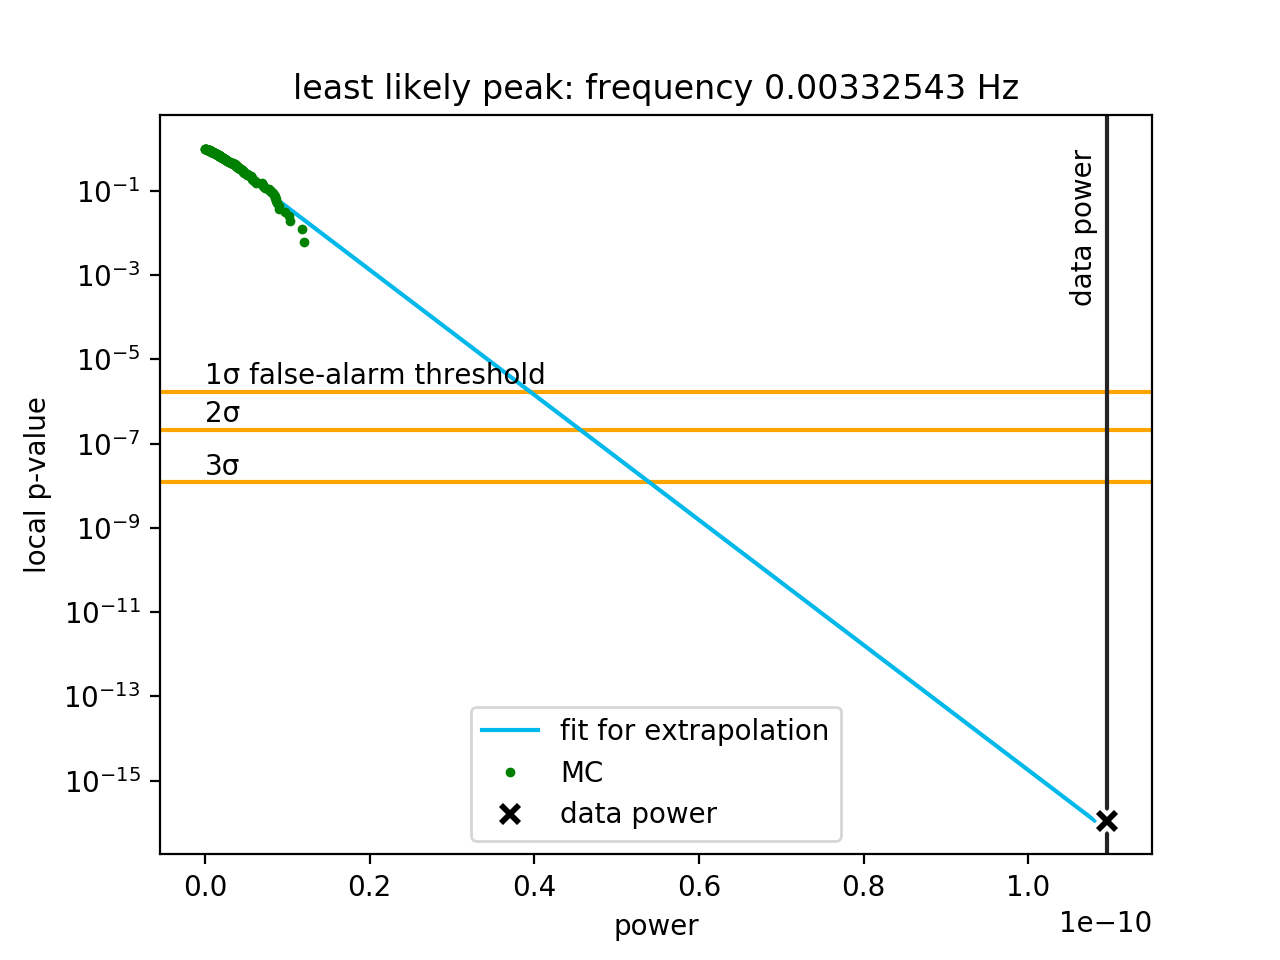
\includegraphics[width=0.9\linewidth]{gfx/axions/P_best_signal_candidate.png}
  \caption{1 - CDF for the parallel data set. This provides the power to local p-value transition, for each frequency separately. The extrapolation based on Eq.\ldots is shown.}
  \label{fig:P_best_signal_candidate}
\end{figure}

Once every MC-generated power estimate has a local p-value associated with it, we find for each generated periodogram the minimal local p-value and treat it as a statistic in itself. We estimate the CDF of the minimal local p-value. The result is plotted in Fig.\,\ref{fig:P_look-elsewhere}. The plot can be understood in the following way: it states how probable it is (y-axis) for a peak of a given local significance (x-axis) to occur anywhere in a periodogram. In other words, the y-axis corresponds to the \emph{global} p-value. The global p-value for an $n\,\sigma$ level is given by:
\begin{equation}
  \mathrm{erfc}\left( \frac{n}{\sqrt{2}} \right)\ ,
\end{equation}
where $\mathrm{erfc}$ is the complementary error function (intuitively understood as ``one minus the integral of the gaussion distribution''). We mark the global p-values corresponding to $1,\ldots,5\sigma$ levels and via the CDF find the corresponding local p-value thresholds.

\begin{figure}
  \centering
  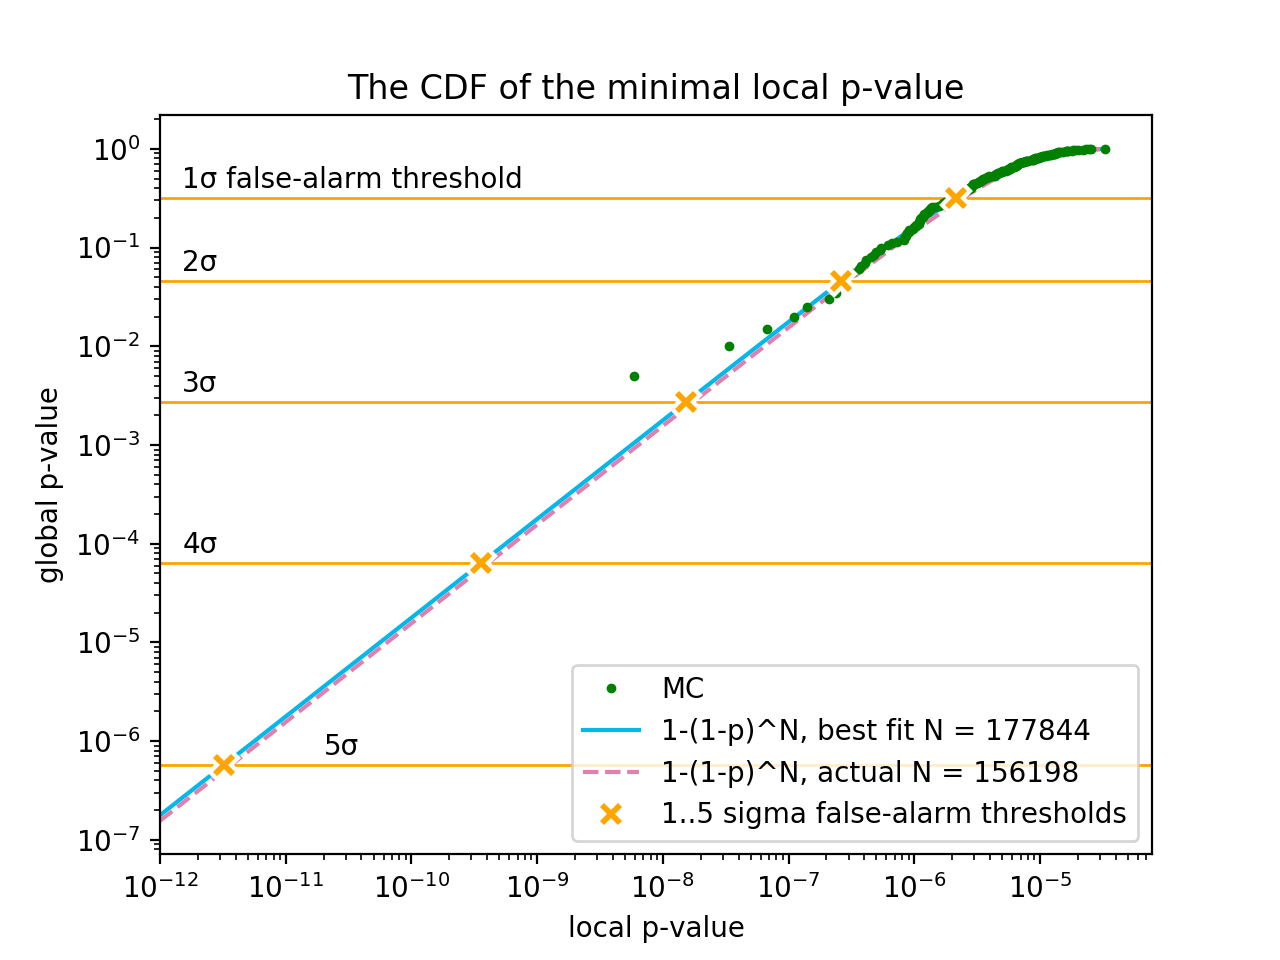
\includegraphics[width=0.9\linewidth]{gfx/axions/P_look-elsewhere.png}
  \caption{Accounting for the look-elsewhere effect for the parallel dataset. It provides the minimal local p-value---global p-value transition. The fit with the model \dots gives the number of frequencies.}
  \label{fig:P_look-elsewhere}
\end{figure}

We see, that the discrete estimate from the MC simulation can only go down to the $2\sigma$ false-alarm threshold. To go lower would require many more MC samples. To observe a single $5\sigma$ event, roughly one-in-a-million, needs typically a million samples. To reduce the computational effort we exploit the fact, that we know the expected functional form of the CDF\@:
\begin{equation}
  F(p) = 1 - (1-p)^N\ ,
\end{equation}
\mnote{Ref.\,for the formula? PDF statistics? Scargle?}
where $N$ is the total number of frequencies. This corresponds to $N$ \emph{independent} statistical tests. We refrain from using for $N$ the actual number of frequencies, \num{156198}, because we cannot guarantee that the power estimates at different frequencies are independent\footnote{They are in a case of periodograms of evenly sampled series}. Instead, we fit $N$ to the observed CDF obtaining \num{177844}. CDFs corresponding to both values of $N$ are depicted in Fig.\,\ref{fig:P_look-elsewhere} and are almost overlapping.

Now for each frequency the local p-values corresponding the the false-alarm thresholds are known. They are depicted in Fig.\,\ref{fig:P_best_signal_candidate}. There, the power CDF (at this frequency) can be used to express the thresholds in power or evaluate the global significance of an arbitrary power. Here, too, the problem is that the discretely estimated CDF does not reach far enough in the tails, and, again, we exploit the functional form to extrapolate the CDF. We expect the power to be exponentially distributed in a no-signal case \cite{Scargle1982}, which corresponds to a straight line on the CDF plot with a logarithmic y-scale.

The thresholds powers are different for each frequency and are depicted in orange in Fig.\,\ref{fig:axions_PSI_detection}. They provide an intuitive interpretation of the plot: the most significant signal candidate is the one piercing furthest into the false-alarm thresholds. Its statistical significance is equal to the last threshold it crossed.



\section{Further discussion}
\mnote{In this paragraph discuss the the distribution of the p-values and plot the filtered p-values.}
\mnote{Now, proceed to discuss the distribution of p-values. Then, proceed to plot the filtered p-values as the function of frequency.}
There are a number of frequencies where statistically significant (put the $\sigma$ level here) excesses are observed in the EB parallel and EB anti-parallel datasets. 
Even though they are not compatible with an axion-induced signal, it is interesting to investigate the possible reason.

In the first step we look at the p-value distribution, shown in black in Fig.\,\ref{fig:axions_P_p-values} (for the EB parallel dataset).
\mnote{Come up with a nice name for the EB parallel and anti-parallel data sets.}
The distribution is flat with narrow peak in the first bin, corresponding to the highest excesses.
This means that there is only a small number (around 300) frequencies, where more power than expected is observed.
\marginpar{A global, like over- or underestimating the error-bars, would cause a tilt in the p-value distribution.}
To identify this group we plot the ratio of the observed to average amplitude (Fig.\,\ref{fig:axions_observed-predicted_power_ratio_filtered}). The lines are low-pass filtered to average the statistical noise out. The excesses occur only for frequencies below \SI{1e-4}{\hertz} and in a narrow region around inverse \SI{300}{\second}. These are the regions where the gradient-drift correction had an effect.

Here tell how it might be due to the imperfect gradient-drift correction. Say, that the narrow region around inverse \SI{300}{\second} is most likely strongly correlated with the low frequencies (essentially peak folding around the Nyquist frequency in the case of evenly sampled data.)


\begin{figure}
  \centering
  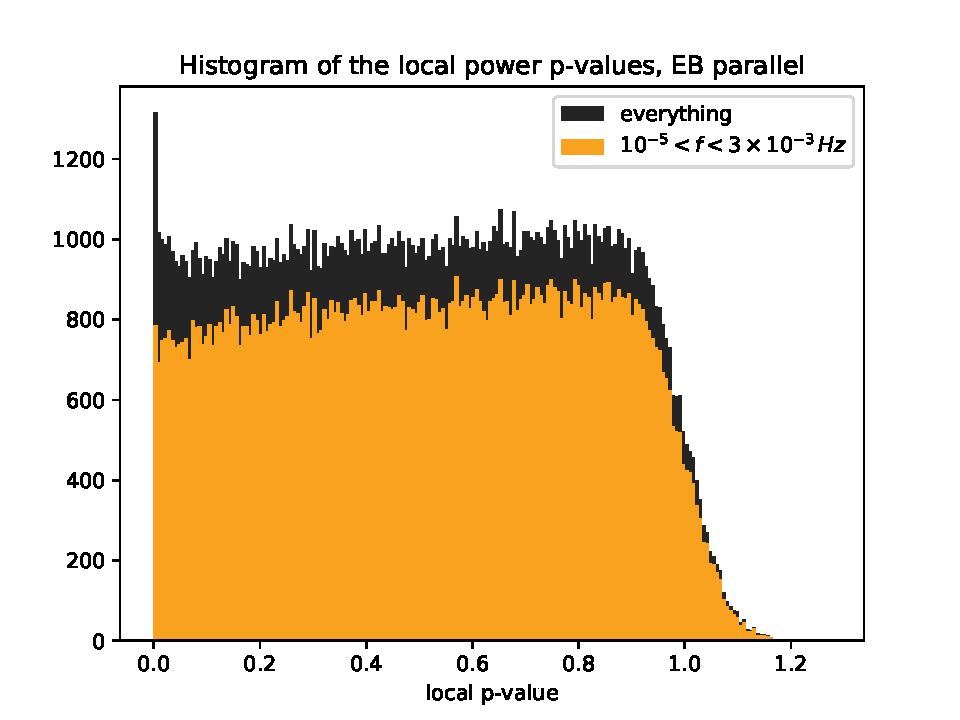
\includegraphics[width=0.9\linewidth]{gfx/axions/P_p-values.pdf}
  \caption{Accounting for the look-elsewhere effect for the parallel dataset. It provides the minimal local p-value -- global p-value transition. The fit with the model \dots gives the number of frequencies. \note{Prepare this histogram in a way, that the curves for all the datasets are shown. Then may need to normalise it.}}
  \label{fig:axions_P_p-values}
\end{figure}

\begin{figure}
  \centering
  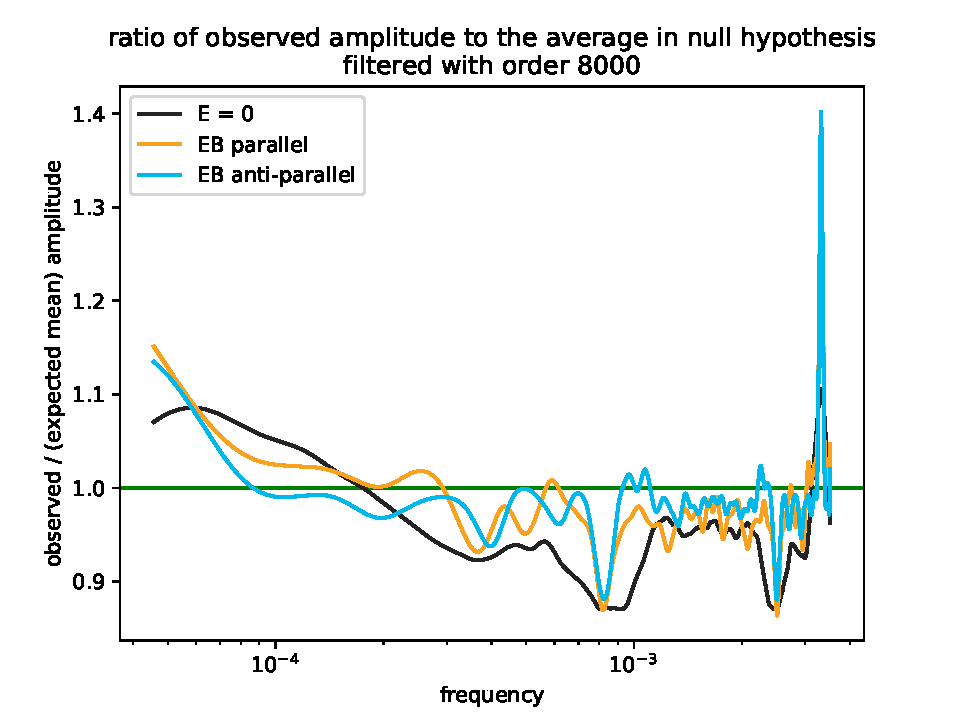
\includegraphics[width=0.9\linewidth]{gfx/axions/observed-predicted_power_ratio_filtered.pdf}
  \caption{Maybe mark the 1/300 seconds. Note, that because of the settling of the filter first $N$ points need to be dropped, so not whole range is plotted.}
  \label{fig:axions_observed-predicted_power_ratio_filtered}
\end{figure}



\section{Axion-Wind analysis}
The analysis described in this chapter so far concerned the scalar coupling of the axions to gluons, which looks like an oscillation in the electric dipole moment of the neutron.
Now we describe how we used the same data set and the same analysis techniques to look for a different coupling --- a vector one of axions to nucleons.

\begin{figure}
  \centering
  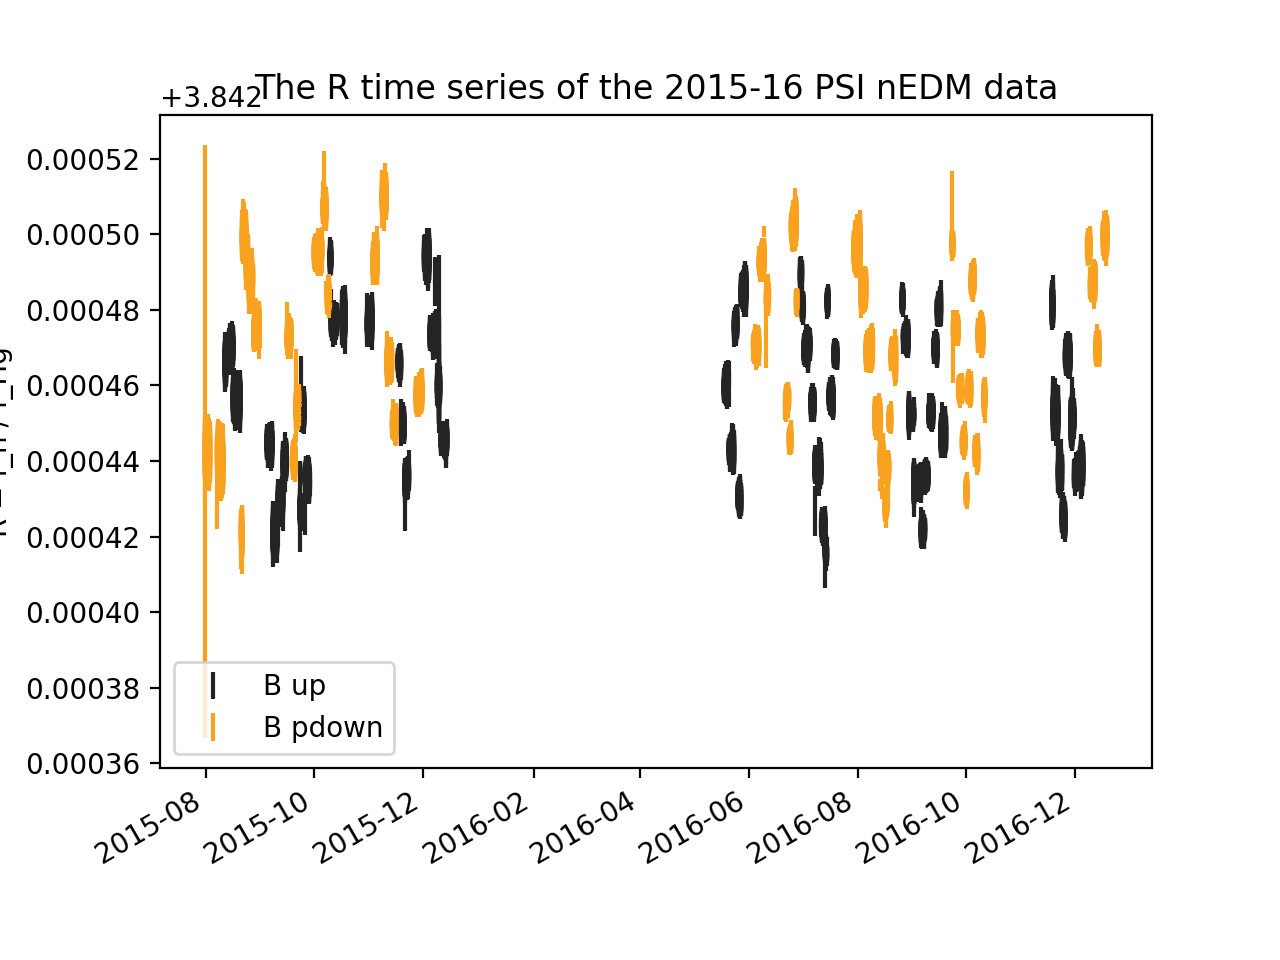
\includegraphics[width=0.9\linewidth]{gfx/axions/winddeltah4mm_time_domain.png}
  \caption{\ldots}
  \label{fig:axions_wind_time_domain}
\end{figure}

This coupling acts like an additional dynamic magnetic field. In this analysis the data are split based on the direction of the holding magnetic field $B_0$, as indicated in Fig.\,\ref{fig:axions_wind_time_domain}. The axion-wind coupling is insensitive to the electric field in the experiment.

The axion-wind coupling \note{ref to equation} is proportional to the projection of experiment's quantisation axis on the momentum of the axions.
Because the latter is due to the Earth traversing the galactic axion field in the Solar System's movement around the Milky Way's centre, the effect is called Axion-Wind. \note{Maybe a ref}
The Earth additionally spins, causing the effect to be modulated with the sidereal frequency $\Omega_\mathrm{sid}$.\footnote{Sidereal frequency is one of the Earth's spinning as seen in the reference of fixed stars.}
The modulation makes a signal in periodogram a triplet, with the central, highest, peak at the frequency of the oscillation of the axion field, and two additional ones, on either side, $\Omega_\mathrm{sid}$ away from the main peak.

Besides splitting the data on the direction of the magnetic field, rather than the relative direction of the magnetic and electric ones, the analysis is performed exactly in the same way as in the case of the search for the scalar axion-gluon coupling. The periodograms for the two datasets are presented in Fig.\,\ref{fig:axions_wind_Bup_detection} (magnetic field pointing upwards, relative to gravity) and Fig.\,\ref{fig:axions_wind_Bdown_detection} (pointing downwards).

\begin{figure}
  \centering
  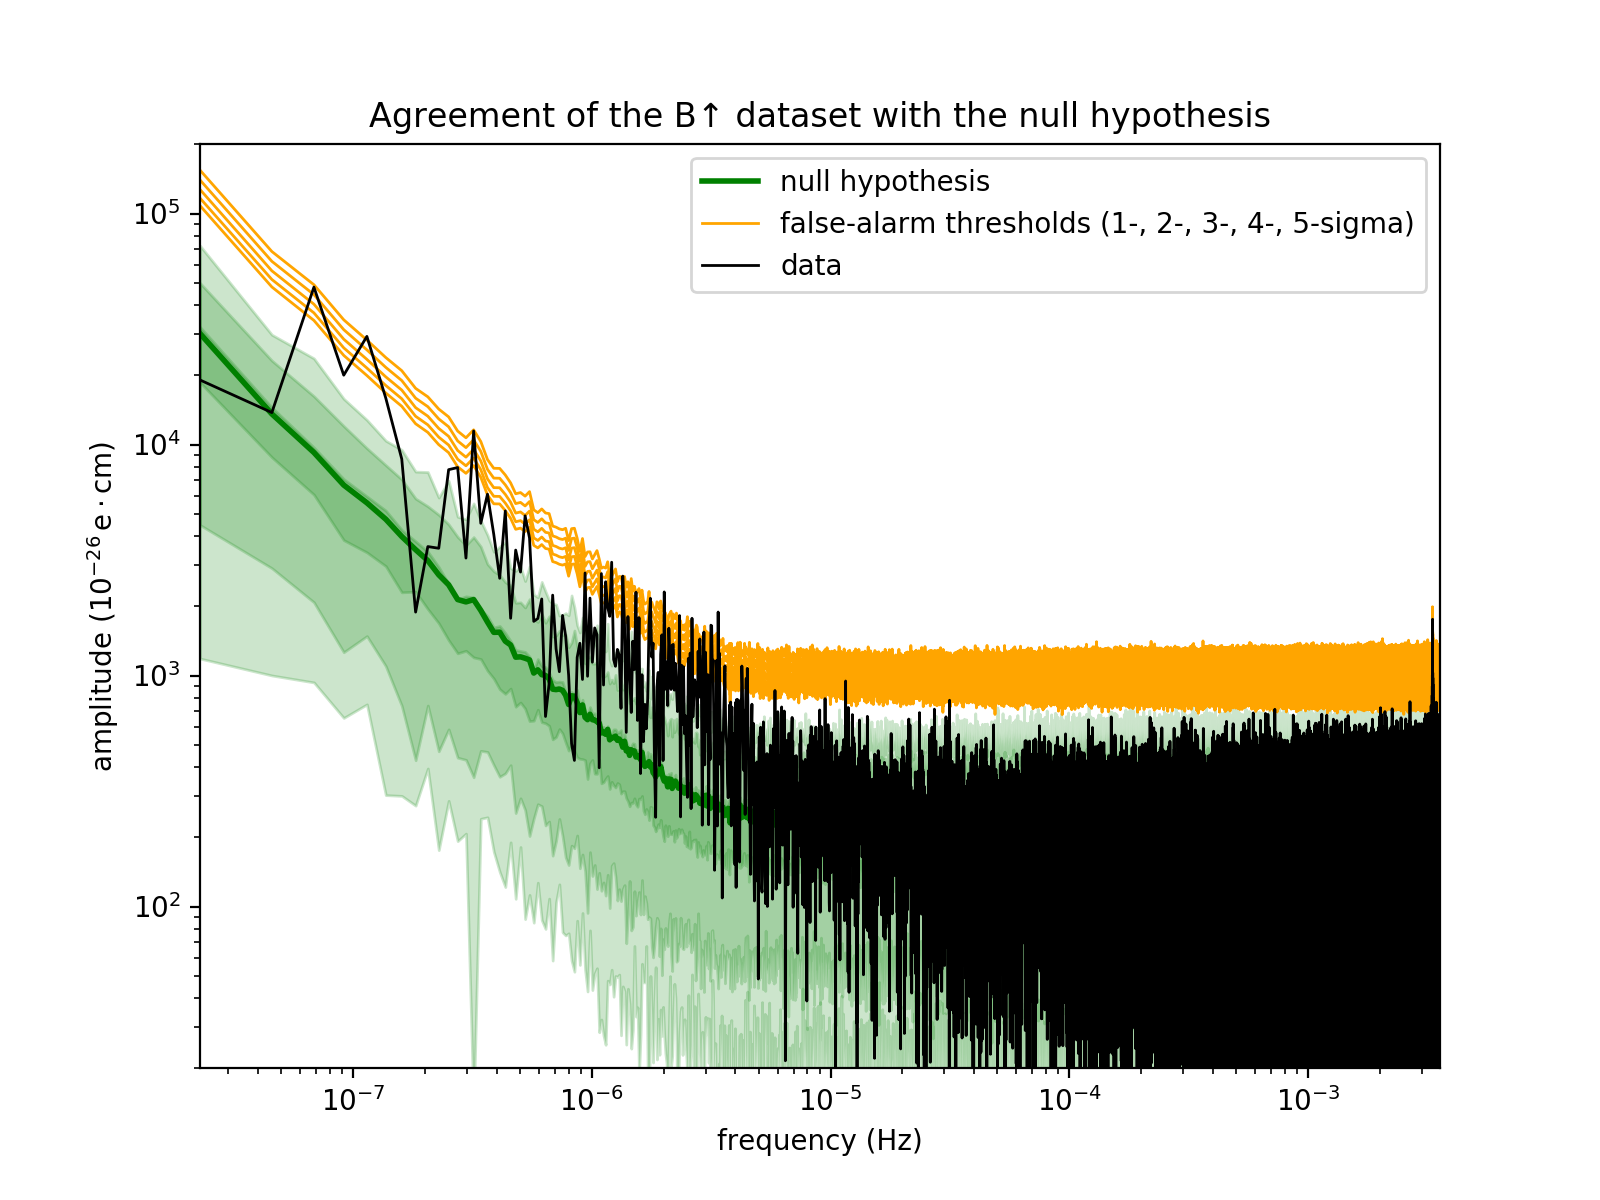
\includegraphics[width=0.9\linewidth]{gfx/axions/winddeltah4mm_Bup_detection.png}
  \caption{Maybe mark the 1/300 seconds. Note, that because of the settling of the filter first $N$ points need to be dropped, so not whole range is plotted.}
  \label{fig:axions_wind_Bup_detection}
\end{figure}

\begin{figure}
  \centering
  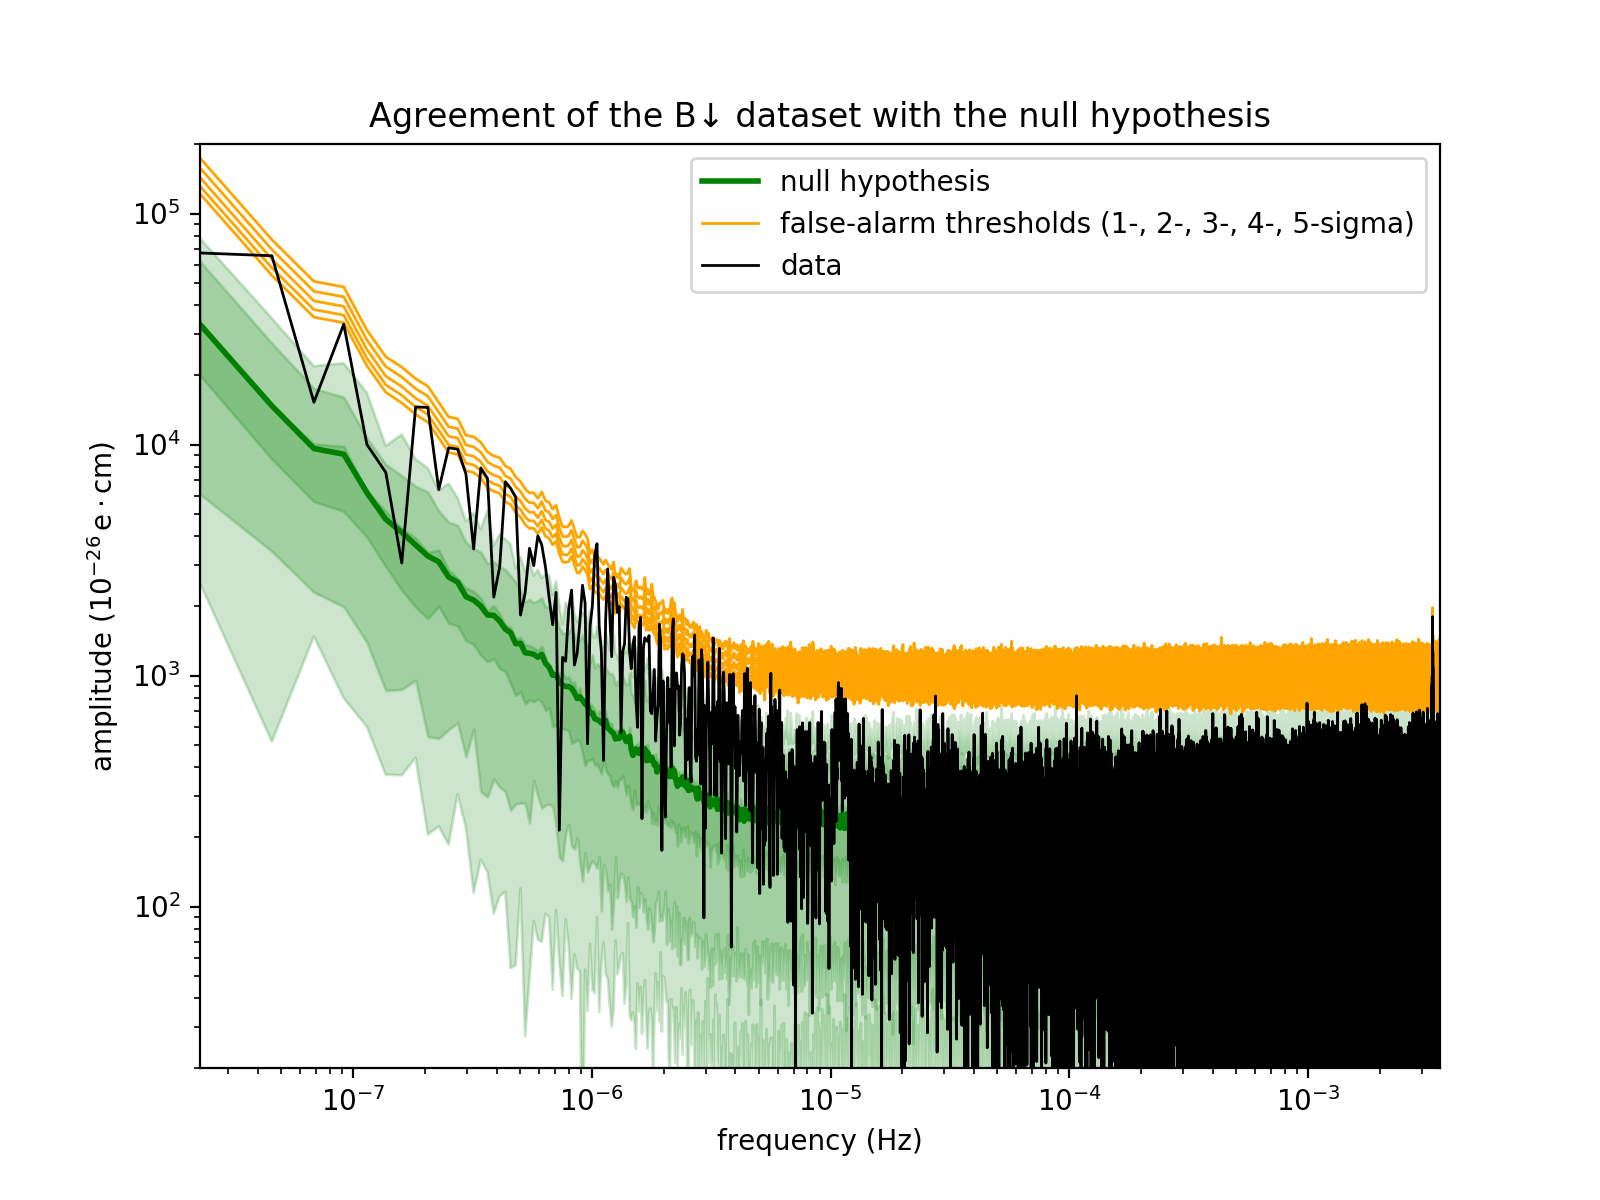
\includegraphics[width=0.9\linewidth]{gfx/axions/winddeltah4mm_Bdown_detection.png}
  \caption{\ldots}
  \label{fig:axions_wind_Bdown_detection}
\end{figure}

We see a lot of excesses (figures, already gradient-drift corrected), but none passes the detection criteria (the phase requirements in particular).

The lack of statistically significant signal compatible with the axion model allowed us to put limits on the axion-nucleon coupling, depicted in Fig.\,\ref{fig:axions_wind_limits}. \note{comment a bit on the other limits in the plot}

\begin{figure}
  \centering
  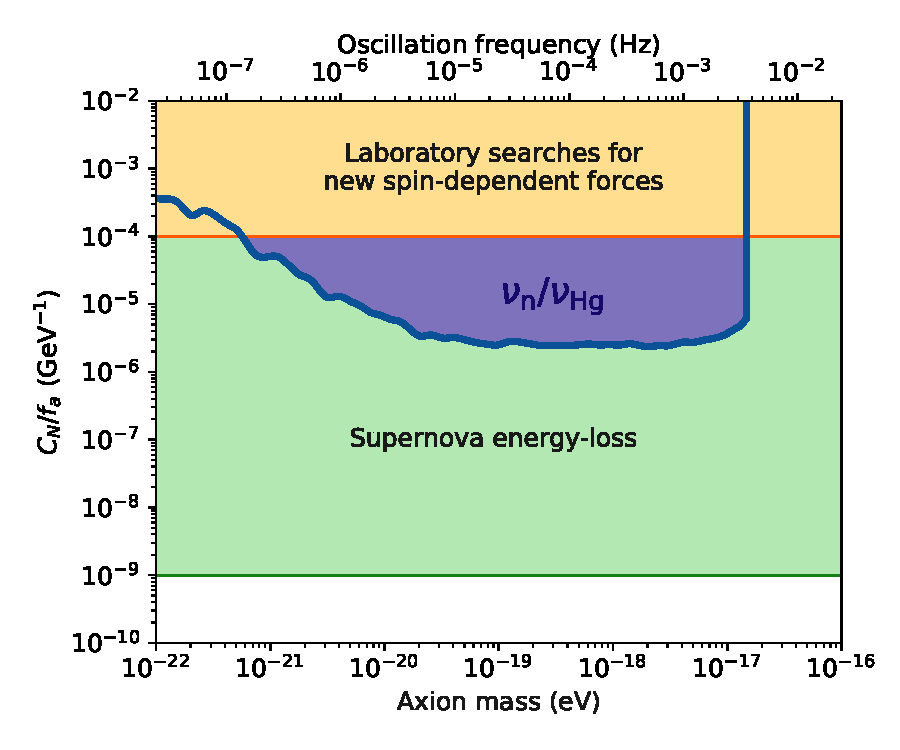
\includegraphics[width=0.9\linewidth]{gfx/axions/psi_ill_axion_wind_limits_v1.pdf}
  \caption{\ldots}
  \label{fig:axions_wind_limits}
\end{figure}



\section{Sidereal frequency}
A note about the signals seen at this particular frequency. Refer to the Lorentz-invariance paper, improve the limit directly? \cite{ALTAREV20112365}



\section{Outlook}
There are three direction in which the nEDM-based axion dark matter search could continue.
To improve sensitivity vertically (be sensitive to more weekly coupled or less abundant axions) the overall sensitivty of the nEDM measurement would need to be improved.
Following the Eq\,\note{ref to the nEDM sensitivity formula}: more neutrons or higher electric field.
\marginpar{In Eq. $\alpha$ is already \ldots, precession time $T$ can only be improved so long --- it is fundamentally limited by the neutron life-time (give the number.)}
The global community already spares no effort to achieve that.
The second way is to improve sensitivity for slower oscillations, or lighter axions, limited by the span of the data set. For this analysis this are the four years of the ILL measurement. Combining the ILL and PSI data into one time series would improve it to \note{number}. It was not done at the time, because the PSI data were still blinded and the run-level analysis was still ongoing.
The third direction is the high-frequency, heavy-axions one. It is limited by the sampling frequency fo the system, the cycle repetition rate. The measurements could be conducted with a shorter cycle time (worsening the sensitivity, as the loss in Eq.\,\note{ref the nEDM sensitivity} is linear, and the gain from the statistics is a square root).
\marginpar{In PSI the cycles are synchronised to the pulses of the kicker magnet, redirecting the proton beam onto the target of the UCN source.}
However, it is hard to imagine going beyond ten-second range. A real improvement in this direction would require changing the principle of the measurement.




\section{Resonant oscillating nEDM search}
Many of the axion searches are resonant based. \note{some references}.
The standard instrument to look for an axion-photon coupling, called a haloscope \note{verity}, consists of ultra-low-noise resonant cavity, where axions can produce photons, detected with an antenna \note{is it an antenna?}.
At any given time the measurement is sensitive only to a narrow band of photon energies (or frequencies), the width given by the finesse \note{verity} of the cavity. To cover a wide range the tuning of the cavity is scanned. In this section an idea of a resonant oscillating nEDM search is pursued.

For polarised neturons in a magnetic field, a transverse oscillating coupling induces a coherent Rabi oscillation between the spin-up and spin-down states.
For example, a Ramsey cycle begins with a $\uppi$/2 flip, induced by an oscillating transverse magnetic field, its frequency tuned to the Larmor one and its length tuned such, that the Rabi oscillation stops when the polarisation is in the transverse plane. Should the nEDM oscillate, an oscillating transverse coupling can be achieved with a static magnetic field \emph{perpendicular} to the holding magnetic field. Then, if the frequency of the nEDM oscillation is tuned to the Larmor one, the neutrons would undergo a Rabi nutation, which could be detected.



First - just scanning.

Broad band possibility? It is like an adiabatic spin-flip, but without the oscillating field. The fact that the spin flip occurs, would indicate a presence of the field.



\part{Misc}
\chapter{Caching scheme}


\ctparttext{You can put some informational part preamble text here. Illo principalmente su nos. Non message \emph{occidental} angloromanic da. Debitas effortio simplificate sia se, auxiliar summarios da que, se avantiate publicationes via. Pan in terra summarios, capital interlingua se que. Al via multo esser specimen, campo responder que da. Le usate medical addresses pro, europa origine sanctificate nos se.} % Text on the Part 1 page describing  the content in Part 1

\part{Some Kind of Manual} % First part of the thesis

% Chapter 1

\chapter{Introduction} % Chapter title

\label{ch:introduction} % For referencing the chapter elsewhere, use \autoref{ch:introduction} 

%----------------------------------------------------------------------------------------

This template for \LaTeX\ has two goals:
\begin{enumerate}
\item Provide students with an easy-to-use template for their Master's or PhD thesis (though it might also be used by other types of authors for reports, books, etc.).
\item Provide a classic, high-quality typographic style that is inspired by \citeauthor{bringhurst:2002}'s ``\emph{The Elements of Typographic Style}'' \citep{bringhurst:2002}.
\marginpar{\myTitle \myVersion}
\end{enumerate}

The bundle is configured to run with a \emph{full} MiK\TeX\ or \TeX Live installation right away and, therefore, it uses only freely available fonts.

People interested only in the nice style and not the whole bundle can now use the style stand-alone via the file \texttt{classicthesis.sty}. This works now also with ``plain'' \LaTeX.

As of version 3.0, \texttt{classicthesis} can also be easily used with \mLyX\footnote{\url{http://www.lyx.org}} thanks to Nicholas Mariette and Ivo Pletikosi\'c. The \mLyX\ version of this manual will contain more information on the details.

This should enable anyone with a basic knowledge of \LaTeXe\ or \mLyX\ to produce beautiful documents without too much effort. In the end, this is my overall goal: more beautiful documents, especially theses, as I am tired of seeing so many ugly ones.

The whole template and the used style is released under the \textsmaller{GNU} General Public License. 

If you like the style then I would appreciate a postcard:
\begin{center}
Andre Miede \\
Detmolder Strasse 32 \\
31737 Rinteln \\
Germany
\end{center}

\noindent The postcards I received so far are available at:
\begin{center}
 \url{http://postcards.miede.de}
\end{center}
\marginpar{A well-balanced line width improves the legibility of the text. That's what typography is all about, right?} So far, many theses, some books, and several other publications have been typeset successfully with it. If you are interested in some typographic details behind it, enjoy Robert Bringhurst's wonderful book. % \citep{bringhurst:2002}.

\paragraph{Important Note:} Some things of this style might look unusual at first glance, many people feel so in the beginning. However, all things are intentionally designed to be as they are, especially these:
\begin{itemize}
\item No bold fonts are used. Italics or spaced small caps do the job quite well.
\item The size of the text body is intentionally shaped like it is. It supports both legibility and allows a reasonable amount of information to be on a page. And, no: the lines are not too short.
\item The tables intentionally do not use vertical or double rules. See the documentation for the \texttt{booktabs} package for a nice discussion of this topic.\footnote{To be found online at \\ \url{http://www.ctan.org/tex-archive/macros/latex/contrib/booktabs/}.}
\item And last but not least, to provide the reader with a way easier access to page numbers in the table of contents, the page numbers are right behind the titles. Yes, they are \emph{not} neatly aligned at the right side and they are \emph{not} connected with dots that help the eye to bridge a distance that is not necessary. If you are still not convinced: is your reader interested in the page number or does she want to sum the numbers up?
\end{itemize}

\noindent Therefore, please do not break the beauty of the style by changing these things unless you really know what you are doing! Please.

%----------------------------------------------------------------------------------------

\section{Organization}
A very important factor for successful thesis writing is the organization of the material. This template suggests a structure as the following:
\begin{itemize}
\marginpar{You can use these margins for summaries of the text body\dots}
\item\texttt{Chapters/} is where all the ``real'' content goes in separate files such as \texttt{Chapter01.tex} etc.
\item\texttt{FrontBackMatter/} is where all the stuff goes that surrounds the ``real'' content, such as the acknowledgments, dedication, etc.
\item\texttt{gfx/} is where you put all the graphics you use in the thesis. Maybe they should be organized into subfolders depending on the chapter they are used in, if you have a lot of graphics.
\item\texttt{Bibliography.bib}: the Bib\TeX\ database to organize all the references you might want to cite.
\item\texttt{classicthesis.sty}: the style definition to get this awesome look and feel. Bonus: works with both \LaTeX\ and \textsc{pdf}\LaTeX\dots and \mLyX.
\item\texttt{ClassicThesis.tcp} a \TeX nicCenter project file. Great tool and it's free!
\item\texttt{ClassicThesis.tex}: the main file of your thesis where all the content gets bundled together.
\item\texttt{classicthesis-config.tex}: a central place to load all nifty packages that are used. In there, you can also activate backrefs in order to have information in the bibliography about where a source was cited in the text (\ie, the page number).
    
\emph{Make your changes and adjustments here.} This means that you specify here the options you want to load \texttt{classicthesis.sty} with. You also adjust the title of your thesis, your name, and all similar information here. Refer to \autoref{sec:custom} for more information.

This had to change as of version 3.0 in order to enable an easy transition from the ``basic'' style to \mLyX.
\end{itemize}

\noindent In total, this should get you started in no time.

%----------------------------------------------------------------------------------------

\section{Style Options}\label{sec:options}

There are a couple of options for \texttt{classicthesis.sty} that allow for a bit of freedom concerning the layout: \marginpar{\dots or your supervisor might use the margins for some comments of her own while reading.}
\begin{itemize}
\item General:
\begin{itemize}
\item\texttt{drafting}: prints the date and time at the bottom of each page, so you always know which version you are dealing with. Might come in handy not to give your Prof. that old draft.
\end{itemize}
	
\item Parts and Chapters:
\begin{itemize}
\item\texttt{parts}: if you use Part divisions for your document, you should choose this option. (Cannot be used together with \texttt{nochapters}.)

\item\texttt{nochapters}: allows to use the look-and-feel with classes that do not use chapters, \eg, for articles. Automatically turns off a couple of other options: \texttt{eulerchapternumbers}, \texttt{linedheaders}, \texttt{listsseparated}, and \texttt{parts}. 

\item\texttt{linedheaders}: changes the look of the chapter headings a bit by adding a horizontal line above the chapter title. The chapter number will also be moved to the top of the page, above the chapter title.
\end{itemize}

\item Typography:
\begin{itemize}
\item\texttt{eulerchapternumbers}: use figures from Hermann Zapf's Euler math font for the chapter numbers. By default, old style figures from the Palatino font are used.

\item\texttt{beramono}: loads Bera Mono as typewriter font. (Default setting is using the standard CM typewriter font.)
\item\texttt{eulermath}: loads the awesome Euler fonts for math. (Palatino is used as default font.)

\item\texttt{pdfspacing}: makes use of pdftex' letter spacing capabilities via the \texttt{microtype} package.\footnote{Use \texttt{microtype}'s \texttt{DVIoutput} option to generate DVI with pdftex.} This fixes some serious issues regarding math formul\ae\ etc. (\eg, ``\ss'') in headers. 

\item\texttt{minionprospacing}: uses the internal \texttt{textssc} command of the \texttt{MinionPro} package for letter spacing. This automatically enables the \texttt{minionpro} option and overrides the \texttt{pdfspacing} option.
\end{itemize}  

\item Table of Contents:
\begin{itemize}
\item\texttt{tocaligned}: aligns the whole table of contents on the left side. Some people like that, some don't.

\item\texttt{dottedtoc}: sets pagenumbers flushed right in the table of contents.

\item\texttt{manychapters}: if you need more than nine chapters for your document, you might not be happy with the spacing between the chapter number and the chapter title in the Table of Contents. This option allows for additional space in this context. However, it does not look as ``perfect'' if you use \verb|\parts| for structuring your document.
\end{itemize}

\item Floats:
\begin{itemize}
\item\texttt{listings}: loads the \texttt{listings} package (if not already done) and configures the List of Listings accordingly.
    
\item\texttt{floatperchapter}: activates numbering per chapter for all floats such as figures, tables, and listings (if used).	
    
\item\texttt{subfig}(\texttt{ure}): is passed to the \texttt{tocloft} package to enable compatibility with the \texttt{subfig}(\texttt{ure}) package. Use this option if you want use classicthesis with the \texttt{subfig} package.

\end{itemize}    

\end{itemize}

\noindent The best way to figure these options out is to try the different possibilities and see, what you and your supervisor like best.

In order to make things easier in general, \texttt{classicthesis-config.tex} contains some useful commands that might help you.

%----------------------------------------------------------------------------------------

\section{Customization}\label{sec:custom}

This section will give you some hints about how to adapt \texttt{classicthesis} to your needs.

The file \texttt{classicthesis.sty} contains the core functionality of the style and in most cases will be left intact, whereas the file \texttt{classic\-thesis-config.tex} is used for some common user customizations. 

The first customization you are about to make is to alter the document title, author name, and other thesis details. In order to do this, replace the data in the following lines of \texttt{classicthesis-config.tex:}\marginpar{Modifications in \texttt{classic\-thesis-config.tex}
}

\begin{lstlisting}[frame=lt]
\newcommand{\myTitle}{A Classic Thesis Style\xspace}
\newcommand{\mySubtitle}{An Homage to ...\xspace}
\newcommand{\myDegree}{Doktor-Ingenieur (Dr.-Ing.)\xspace}
\end{lstlisting}

Further customization can be made in \texttt{classicthesis-config.tex} by choosing the options to \texttt{classicthesis.sty} (see~\autoref{sec:options}) in a line that looks like this:

\begin{lstlisting}[frame=lt]
\PassOptionsToPackage{eulerchapternumbers,listings,drafting, pdfspacing, subfig,beramono,eulermath,parts}{classicthesis}

\end{lstlisting}

If you want to use backreferences from your citations to the pages they were cited on, change the following line from:
\begin{lstlisting}[breaklines=false,frame=lt]
\setboolean{enable-backrefs}{false}
\end{lstlisting}
to
\begin{lstlisting}[breaklines=false,frame=lt]
\setboolean{enable-backrefs}{true}
\end{lstlisting}

Many other customizations in \texttt{classicthesis-config.tex} are possible, but you should be careful making changes there, since some changes could cause errors.

Finally, changes can be made in the file \texttt{classicthesis.sty}, \marginpar{Modifications in \texttt{classicthesis.sty}} although this is mostly not designed for user customization. The main change that might be made here is the text-block size, for example, to get longer lines of text.

%----------------------------------------------------------------------------------------

\section{Issues}\label{sec:issues}
This section will list some information about problems using \texttt{classic\-thesis} in general or using it with other packages.

Beta versions of \texttt{classicthesis} can be found at the following Google code repository:
\begin{center}
\url{http://code.google.com/p/classicthesis/}
\end{center}

\noindent There, you can also post serious bugs and problems you encounter.

\subsection*{Compatibility with the \texttt{glossaries} Package}
If you want to use the \texttt{glossaries} package, take care of loading it with the following options:
\begin{verbatim}
\usepackage[style=long,nolist]{glossaries}
\end{verbatim}

\noindent Thanks to Sven Staehs for this information. 

\subsection*{Compatibility with the (Spanish) \texttt{babel} Package}
Spanish languages need an extra option in order to work with this template:
\begin{verbatim}
\usepackage[spanish,es-lcroman]{babel}
\end{verbatim}

\noindent Thanks to an unknown person for this information (via Google Code issue reporting). 

\subsection*{Compatibility with the \texttt{pdfsync} Package}
Using the \texttt{pdfsync} package leads to linebreaking problems with the \texttt{graffito} command. Thanks to Henrik Schumacher for this information. 

%----------------------------------------------------------------------------------------

\section{Future Work}
So far, this is a quite stable version that served a couple of people well during their thesis time. However, some things are still not as they should be. Proper documentation in the standard format is still missing. In the long run, the style should probably be published separately, with the template bundle being only an application of the style. Alas, there is no time for that at the moment\dots it could be a nice task for a small group of \LaTeX nicians.

Please do not send me email with questions concerning \LaTeX\ or the template, as I do not have time for an answer. But if you have comments, suggestions, or improvements for the style or the template in general, do not hesitate to write them on that postcard of yours.

%----------------------------------------------------------------------------------------

\section{License}
\paragraph{GNU General Public License:} This program is free software; you can redistribute it and/or modify it under the terms of the \textsmaller{GNU} General Public License as published by the Free Software Foundation; either version 2 of the License, or (at your option) any later version.

This program is distributed in the hope that it will be useful, but \emph{without any warranty}; without even the implied warranty of \emph{merchantability} or \emph{fitness for a particular purpose}. See the \textsmaller{GNU} General Public License for more details. % Chapter 1

\cleardoublepage % Empty page before the start of the next part

%------------------------------------------------

\ctparttext{You can put some informational part preamble text here. Illo principalmente su nos. Non message \emph{occidental} angloromanic da. Debitas effortio simplificate sia se, auxiliar summarios da que, se avantiate publicationes via. Pan in terra summarios, capital interlingua se que. Al via multo esser specimen, campo responder que da. Le usate medical addresses pro, europa origine sanctificate nos se.} % Text on the Part 2 page describing the content in Part 2

\part{The Showcase} % Second part of the thesis

% Chapter 2

\chapter{Examples} % Chapter title

\label{ch:examples} % For referencing the chapter elsewhere, use \autoref{ch:examples}

%----------------------------------------------------------------------------------------

\lipsum[1]

%----------------------------------------------------------------------------------------

\section{A New Section}

\lipsum[2]

Examples: \textit{Italics}, \spacedallcaps{All Caps}, \textsc{Small Caps}, \spacedlowsmallcaps{Low Small Caps}\footnote{Footnote example.}.

%------------------------------------------------

\subsection{Test for a Subsection}

\graffito{Note: The content of this chapter is just some dummy text.}
\lipsum[3-5]

%------------------------------------------------

\subsection{Autem Timeam}

\lipsum[6]

%----------------------------------------------------------------------------------------

\section{Another Section in This Chapter}

\lipsum[7]

Sia ma sine svedese americas. Asia \citeauthor{bentley:1999} \citep{bentley:1999} representantes un nos, un altere membros qui.\footnote{De web nostre historia angloromanic.} Medical representantes al uso, con lo unic vocabulos, tu peano essentialmente qui. Lo malo laborava anteriormente uso.

\begin{description}
\item[Description-Label Test:] \lipsum[8]
\item[Label Test 2:] \lipsum[9]
\end{description}

\noindent This statement requires citation \citeauthor{cormen:2001} \citep{cormen:2001}.

%------------------------------------------------

\subsection{Personas Initialmente}

\lipsum[10]

\subsubsection{A Subsubsection}
\lipsum[11]

\paragraph{A Paragraph Example} \lipsum[12]

\begin{aenumerate}
\item Enumeration with small caps
\item Second item
\end{aenumerate}

\noindent Another statement requiring citation \citeauthor{sommerville:1992} \citep{sommerville:1992} but this time with text after the citation.

\begin{table}
\myfloatalign
\begin{tabularx}{\textwidth}{Xll} \toprule
\tableheadline{labitur bonorum pri no} & \tableheadline{que vista}
& \tableheadline{human} \\ \midrule
fastidii ea ius & germano &  demonstratea \\
suscipit instructior & titulo & personas \\
\midrule
quaestio philosophia & facto & demonstrated \citeauthor{knuth:1976} \\
\bottomrule
\end{tabularx}
\caption[Autem timeam deleniti usu id]{Autem timeam deleniti usu id. \citeauthor{knuth:1976}}
\label{tab:example}
\end{table}

\enlargethispage{2cm}

%------------------------------------------------

\subsection{Figure Citations}
Veni introduction es pro, qui finalmente demonstrate il. E tamben anglese programma uno. Sed le debitas demonstrate. Non russo existe o, facite linguistic registrate se nos. Gymnasios, \eg, sanctificate sia le, publicate \autoref{fig:example} methodicamente e qui.

Lo sed apprende instruite. Que altere responder su, pan ma, \ie, signo studio. \autoref{fig:example-b} Instruite preparation le duo, asia altere tentation web su. Via unic facto rapide de, iste questiones methodicamente o uno, nos al.

% \begin{figure}[bth]
% \myfloatalign
% \subfloat[Asia personas duo.]
% {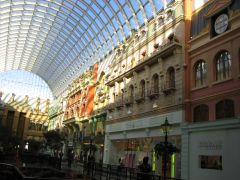
\includegraphics[width=.45\linewidth]{gfx/example_1}} \quad
% \subfloat[Pan ma signo.]
% {\label{fig:example-b}
% 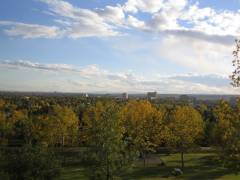
\includegraphics[width=.45\linewidth]{gfx/example_2}} \\
% \subfloat[Methodicamente o uno.]
% {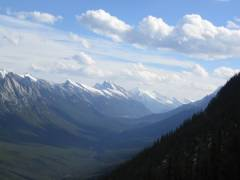
\includegraphics[width=.45\linewidth]{gfx/example_3}} \quad
% \subfloat[Titulo debitas.]
% {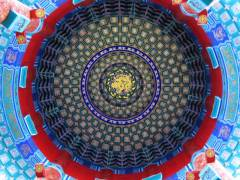
\includegraphics[width=.45\linewidth]{gfx/example_4}}
% \caption[Tu duo titulo debitas latente]{Tu duo titulo debitas latente.}\label{fig:example}
% \end{figure}
 % Chapter 2
% Chapter 3

\chapter{Math Test Chapter} % Chapter title

\label{ch:mathtest} % For referencing the chapter elsewhere, use \autoref{ch:mathtest}

%----------------------------------------------------------------------------------------

\lipsum[13]

%----------------------------------------------------------------------------------------

\section{Some Formulas}

Due to the statistical nature of ionisation energy loss, large fluctuations can occur in the amount of energy deposited by a particle traversing an absorber element\footnote{Examples taken from Walter Schmidt's great gallery: \\ \url{http://home.vrweb.de/~was/mathfonts.html}}.  Continuous processes such as multiple scattering and energy loss play a relevant role in the longitudinal and lateral development of electromagnetic and hadronic showers, and in the case of sampling calorimeters the measured resolution can be significantly affected by such fluctuations in their active layers.  The description of ionisation fluctuations is characterised by the significance parameter $\kappa$, which is proportional to the ratio of mean energy loss to the maximum allowed energy transfer in a single collision with an atomic electron: \graffito{You might get unexpected results using math in chapter or section heads. Consider the \texttt{pdfspacing} option.}
\begin{equation}
\kappa =\frac{\xi}{E_{\mathrm{max}}} %\mathbb{ZNR}
\end{equation}
$E_{\mathrm{max}}$ is the maximum transferable energy in a single collision with an atomic electron.
\[E_{\mathrm{max}} =\frac{2 m_{\mathrm{e}} \beta^2\gamma^2 }{1 + 2\gamma m_{\mathrm{e}}/m_{\mathrm{x}} + \left ( m_{\mathrm{e}} /m_{\mathrm{x}}\right)^2}\ ,\]
where $\gamma = E/m_{\mathrm{x}}$, $E$ is energy and $m_{\mathrm{x}}$ the mass of the incident particle, $\beta^2 = 1 - 1/\gamma^2$ and $m_{\mathrm{e}}$ is the electron mass. $\xi$ comes from the Rutherford scattering cross section and is defined as:
\begin{eqnarray*} \xi  = \frac{2\pi z^2 e^4 N_{\mathrm{Av}} Z \rho
\delta x}{m_{\mathrm{e}} \beta^2 c^2 A} =  153.4 \frac{z^2}{\beta^2}
\frac{Z}{A}
\rho \delta x \quad\mathrm{keV},
\end{eqnarray*}
where

\begin{tabular}{ll}
$z$ & charge of the incident particle \\
$N_{\mathrm{Av}}$ & Avogadro's number \\
$Z$ & atomic number of the material \\
$A$ & atomic weight of the material \\
$\rho$ & density \\
$ \delta x$ & thickness of the material \\
\end{tabular}

$\kappa$ measures the contribution of the collisions with energy transfer close to $E_{\mathrm{max}}$.  For a given absorber, $\kappa$ tends towards large values if $\delta x$ is large and/or if $\beta$ is small.  Likewise, $\kappa$ tends towards zero if $\delta x $ is small and/or if $\beta$ approaches $1$.

The value of $\kappa$ distinguishes two regimes which occur in the description of ionisation fluctuations:

\begin{enumerate}
\item A large number of collisions involving the loss of all or most of the incident particle energy during the traversal of an absorber.

As the total energy transfer is composed of a multitude of small energy losses, we can apply the central limit theorem and describe the fluctuations by a Gaussian distribution. This case is applicable to non-relativistic particles and is described by the inequality $\kappa > 10 $ (\ie, when the mean energy loss in the absorber is greater than the maximum energy transfer in a single collision).

\item Particles traversing thin counters and incident electrons under any conditions.

The relevant inequalities and distributions are $ 0.01 < \kappa < 10 $, Vavilov distribution, and $\kappa < 0.01 $, Landau distribution.
\end{enumerate}

%----------------------------------------------------------------------------------------

\section{Various Mathematical Examples}

If $n > 2$, the identity \[t[u_1,\dots,u_n] = t\bigl[t[u_1,\dots,u_{n_1}], t[u_2,\dots,u_n] \bigr]\] defines $t[u_1,\dots,u_n]$ recursively, and it can be shown that the alternative definition \[t[u_1,\dots,u_n] = t\bigl[t[u_1,u_2],\dots,t[u_{n-1},u_n]\bigr]\] gives the same result. % Chapter 3
%% Chapter X

\chapter{Chapter Title} % Chapter title

\label{ch:name} % For referencing the chapter elsewhere, use \autoref{ch:name} 

%----------------------------------------------------------------------------------------

\section{Section Title}

Content

%------------------------------------------------

\subsection{Subsection Title}

Content

%------------------------------------------------

\subsection{Subsection Title}

Content

%----------------------------------------------------------------------------------------

\section{Section Title}

Content % Chapter 4 - empty template

%----------------------------------------------------------------------------------------
%	THESIS CONTENT - APPENDICES
%----------------------------------------------------------------------------------------

\appendix

\part{Appendix} % New part of the thesis for the appendix

% Appendix A

\chapter{Appendix Test}

%----------------------------------------------------------------------------------------

\lipsum[13-14]

%----------------------------------------------------------------------------------------

\section{Appendix Section Test}
\lipsum[15]

\graffito{More dummy text}
\lipsum[16]

%----------------------------------------------------------------------------------------

\section{Another Appendix Section Test}
\lipsum[17]

\begin{table}
\myfloatalign
\begin{tabularx}{\textwidth}{Xll} \toprule
\tableheadline{labitur bonorum pri no} & \tableheadline{que vista}
& \tableheadline{human} \\ \midrule
fastidii ea ius & germano &  demonstratea \\
suscipit instructior & titulo & personas \\
\midrule
quaestio philosophia & facto & demonstrated \\
\bottomrule
\end{tabularx}
\caption[Autem usu id]{Autem usu id.}
\label{tab:moreexample}
\end{table}

\lipsum[18]

\begin{lstlisting}[float,caption=A floating example]
for i:=maxint to 0 do
begin
{ do nothing }
end;
\end{lstlisting} % Appendix A
%% Appendix X

\chapter{Appendix Title}

%----------------------------------------------------------------------------------------

% Content begins here % Appendix B - empty template

%----------------------------------------------------------------------------------------
%	POST-CONTENT THESIS PAGES
%----------------------------------------------------------------------------------------

\cleardoublepage% Bibliography

\label{app:bibliography} % Reference the bibliography elsewhere with \autoref{app:bibliography}

\manualmark
\markboth{\spacedlowsmallcaps{\bibname}}{\spacedlowsmallcaps{\bibname}} 
\refstepcounter{dummy}

\addtocontents{toc}{\protect\vspace{\beforebibskip}} % Place the bibliography slightly below the rest of the document content in the table of contents
\addcontentsline{toc}{chapter}{\tocEntry{\bibname}}

% \bibliographystyle{plainnat}
\bibliographystyle{apsrev4-1}

\bibliography{Bibliography} % Bibliography

\cleardoublepage% Colophon (a brief description of publication or production notes relevant to the edition)

\pagestyle{empty}

\hfill

\vfill

\pdfbookmark[0]{Colophon}{colophon}

\section*{Colophon}

This document was typeset using the typographical look-and-feel \texttt{classicthesis} developed by Andr\'e Miede. The style was inspired by Robert Bringhurst's seminal book on typography ``\emph{The Elements of Typographic Style}''. \texttt{classicthesis} is available for both \LaTeX\ and \mLyX: 

\begin{center}
\url{http://code.google.com/p/classicthesis/}
\end{center}

\noindent Happy users of \texttt{classicthesis} usually send a real postcard to the author, a collection of postcards received so far is featured here: 

\begin{center}
\url{http://postcards.miede.de/}
\end{center}
 
\bigskip

\noindent\finalVersionString % Colophon

\cleardoublepage% Declaration

\refstepcounter{dummy}
\pdfbookmark[0]{Declaration}{declaration} % Bookmark name visible in a PDF viewer

\chapter*{Declaration} % Declaration section text

\thispagestyle{empty}

Put your declaration here.
\bigskip
 
\noindent\textit{\myLocation, \myTime}

\smallskip

\begin{flushright}
\begin{tabular}{m{5cm}}
\\ \hline
\centering\myName, \today \\
\end{tabular}
\end{flushright}
 % Declaration

%----------------------------------------------------------------------------------------

\end{document}
